\section{Global Trigger Logic}
\label{sec:gtl:global_trigger_logic}
\textbf{Remark:}\\
this description is for version 1.10.6 of Global Trigger Logic.\\

The Global Trigger Logic (\ugtl) firmware contains conditions and Algorithms for trigger decision.

\begin{figure}[htb]
\centering
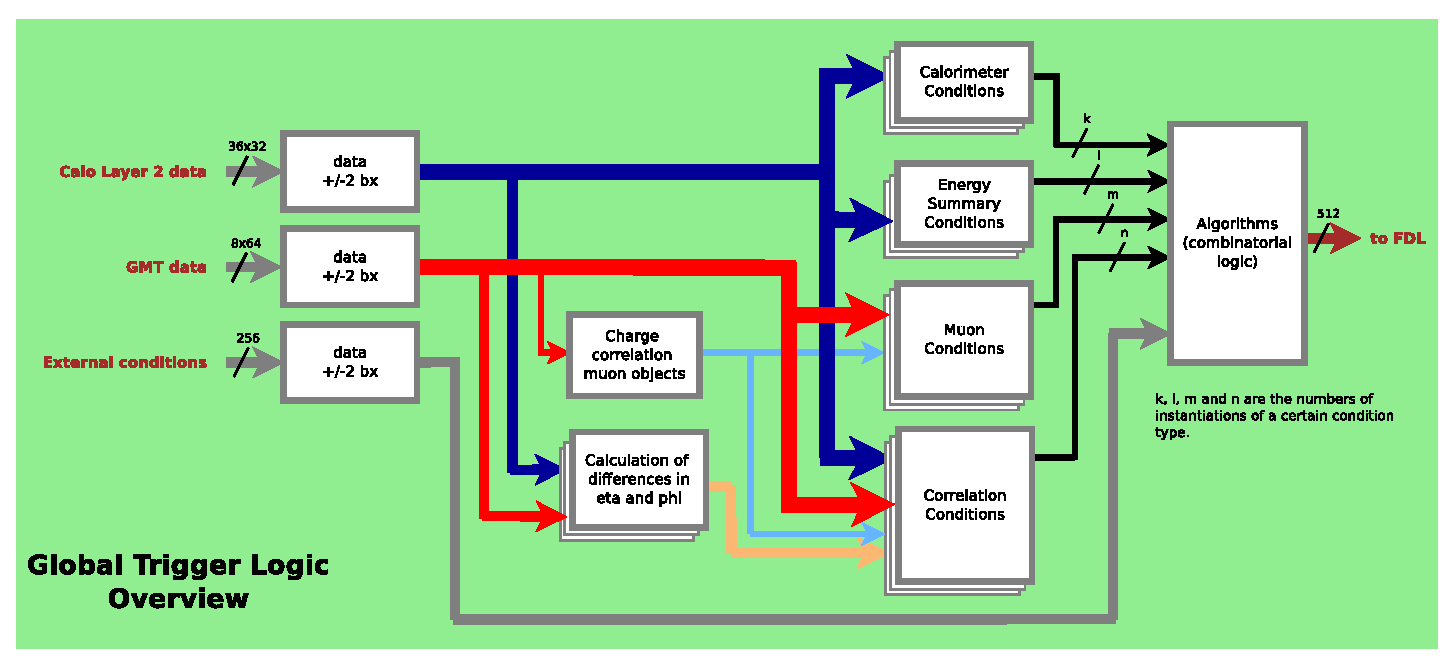
\includegraphics[width=15cm]{figures/mGTL_firmware}
\caption{\ugtl firmware} 
\label{fig:gtl:mGTL_firmware}
\end{figure}

\subsection{\ugtl Interface}
\label{sec:gtl:ugtl_interface}

\textbf{Inputs:}
\begin{itemize}
\item Calo-Layer2 data
\begin{itemize}
\item Electron/$\gamma$ objects
\item Jet objects
\item Tau objects
\item Energy summary information: Total Et (\ett), total Et from ECAL only (ETTEM), total calibrated Et in jets (\htt), missing Et (\etm), missing Et including HF (ET$_{miss}^{HF}$), missing Ht objects (\htm),
missing Ht including HF (HT$_{miss}^{HF}$) and "Asymmetry" information (ASYMET, ASYMHT, ASYMETHF, ASYMHTHF) 
\item Minimum bias HF bits (included in energy summary information data structure)
\item Towercount bits (number of firing HCAL towers, included in energy summary information data structure)
\item "Centrality" bits
\end{itemize}
\item \gmt data
\item External conditions
\item LHC-clock 
\end{itemize}
\textbf{Outputs:}
\begin{itemize}
\item Algorithms
\end{itemize}

\subsection{Definition of optical interfaces}
\label{sec:gtl:optical_interfaces}

Remark: all definitions in the following chapters are from a CMS Detector Note: "Scales for inputs to $\mu$GT" (see actual version in \url{http://globaltrigger.hephy.at/upgrade/ugt/downloads/}).

\subsubsection{Calo-Layer2 optical interfaces}
\label{sec:gtl:gct_optical_interfaces}

The configuration of optical connections from Calo-Layer2 to \ugt is shown in Table~\ref{tab:framework:tab_configuration_optical_conn}.\\
% \textit{The location of the GTH channels for the connections is very preliminary, must be checked with connections on Calo-Layer2.}\\

The data structure of an \egamma object (bits 27..31 are not defined yet, reserved for quality, ...):
\begin{center}
\begin{bytefield}[boxformatting={\centering\itshape}, bitwidth=1.2em, endianness=big]{32}
        \bitheader{0,8,9,16,17,24,25,26,27,31} \\
        \bitbox {5}     {\texttt{qual/spare}} &
        \bitbox {2}     {\texttt{iso}} &
        \bitbox {8}     {\texttt{$\varphi$}}  &
        \bitbox {8}     {\texttt{$\eta$}}  &
        \bitbox {9}     {\texttt{\et}} \\
\end{bytefield}
\end{center}

The data structure of a jet object (bits 27..31 are not defined yet, reserved for quality, ...):
\begin{center}
\begin{bytefield}[boxformatting={\centering\itshape}, bitwidth=1.2em, endianness=big]{32}
        \bitheader{0,10,11,18,19,26,27,31} \\
        \bitbox {5}     {\texttt{iso/qu/sp}} &
        \bitbox {8}     {\texttt{$\varphi$}}  &
        \bitbox {8}     {\texttt{$\eta$}}  &
        \bitbox {11}    {\texttt{\et}} \\
\end{bytefield}
\end{center}

The data structure of a tau object (bits 27..31 are not defined yet, reserved for quality, ...):
\begin{center}
\begin{bytefield}[boxformatting={\centering\itshape}, bitwidth=1.2em, endianness=big]{32}
        \bitheader{0,8,9,16,17,24,25,26,27,31} \\
        \bitbox {5}     {\texttt{qual/spare}} &
        \bitbox {2}     {\texttt{iso}} &
        \bitbox {8}     {\texttt{$\varphi$}}  &
        \bitbox {8}     {\texttt{$\eta$}}  &
        \bitbox {9}     {\texttt{\et}} \\
\end{bytefield}
\end{center}

The data structure of "total Et" (\ett) quantity [including "total Et from ECAL only" (ETTEM) and "minimum bias HF+ threshold 0" bits]:
\begin{center}
\begin{bytefield}[boxformatting={\centering\itshape}, bitwidth=1.2em, endianness=big]{32}
        \bitheader{0,11,12,23,24,27,28,31} \\
        \bitbox {4}    {\texttt{MBT0HFP}} &
        \bitbox {4}    {\texttt{spare}} &
        \bitbox {12}    {\texttt{\et [ETTEM]}} &
        \bitbox {12}    {\texttt{\et [\ett]}} \\
\end{bytefield}
\end{center}

The data structure of "total calibrated Et in jets" (\htt) quantity [including "towercount" and "minimum bias HF- threshold 0" bits]:
\begin{center}
\begin{bytefield}[boxformatting={\centering\itshape}, bitwidth=1.2em, endianness=big]{32}
        \bitheader{0,11,12,24,25,27,28,31} \\
        \bitbox {4}    {\texttt{MBT0HFM}} &
        \bitbox {3}    {\texttt{spare}} &
        \bitbox {13}    {\texttt{TOWERCOUNT}} &
        \bitbox {12}    {\texttt{\et}} \\
\end{bytefield}
\end{center}

The data structure of "missing Et" (\etm) quantity [including "Asymmetry" ASYMET and "minimum bias HF+ threshold 1" bits]:
\begin{center}
\begin{bytefield}[boxformatting={\centering\itshape}, bitwidth=1.2em, endianness=big]{32}
        \bitheader{0,11,12,19,20,27,28,31} \\
        \bitbox {4}    {\texttt{MBT1HFP}} &
        \bitbox {8}    {\texttt{ASYMET}} &
        \bitbox {8}     {\texttt{$\varphi$}} &
        \bitbox {12}    {\texttt{\et}} \\
\end{bytefield}
\end{center}

The data structure of "missing Ht" (\htm) quantity [including "Asymmetry" ASYMHT and "minimum bias HF- threshold 1" bits]:
\begin{center}
\begin{bytefield}[boxformatting={\centering\itshape}, bitwidth=1.2em, endianness=big]{32}
        \bitheader{0,11,12,19,20,27,28,31} \\
        \bitbox {4}    {\texttt{MBT1HFM}} &
        \bitbox {8}    {\texttt{ASYMHT}} &
        \bitbox {8}     {\texttt{$\varphi$}} &
        \bitbox {12}    {\texttt{\et}} \\
\end{bytefield}
\end{center}

The data structure of "missing Et including HF" (ET$_{miss}^{HF}$) quantity [including "Asymmetry" ASYMETHF and "Centrality" bits (3:0)]:
\begin{center}
\begin{bytefield}[boxformatting={\centering\itshape}, bitwidth=1.2em, endianness=big]{32}
        \bitheader{0,11,12,19,20,27,28,31} \\
        \bitbox {4}    {\small  \texttt{[CENT3:0]}} &
        \bitbox {8}    {\texttt{ASYMETHF}} &
        \bitbox {8}     {\texttt{$\varphi$}} &
        \bitbox {12}    {\texttt{\et}} \\
\end{bytefield}
\end{center}

The data structure of "missing Ht including HF" (HT$_{miss}^{HF}$) quantity [including "Asymmetry" ASYMHTHF and "Centrality" bits (7:4)]:
\begin{center}
\begin{bytefield}[boxformatting={\centering\itshape}, bitwidth=1.2em, endianness=big]{32}
        \bitheader{0,11,12,19,20,27,28,31} \\
        \bitbox {4}    {\small  \texttt{CENT[7:4]}} &
        \bitbox {8}    {\texttt{ASYMHTHF}} &
        \bitbox {8}     {\texttt{$\varphi$}} &
        \bitbox {12}    {\texttt{\et}} \\
\end{bytefield}
\end{center}

\subsubsection{\gmt optical interfaces}
\label{sec:gtl:gmt_optical_interfaces}

The data structure of a muon object (64 bits - bit 34 = charge sign, bit 35 = charge valid, bit 61 is a spare bit, bit 63..62 = impact parameter):

\begin{center}
\begin{bytefield}[boxformatting={\centering\itshape}, endianness=big, bitwidth=1.2em]{32}
        \bitheader[lsb=32]{32,33,34,35,36,42,43,52,53,60,61,61,62,63} \\
        \bitbox {2}     {\small  \texttt{imp para}}       &
        \bitbox {1}     {\small  \texttt{r}}       &
        \bitbox {8}     {\texttt{unconst.\pt}}       &
        \bitbox {10}    {\texttt{$\varphi$} (out)}
        \bitbox {7}     {\texttt{index bits}}
        \bitbox {2}     {\small  \texttt{ch}}       &
        \bitbox {2}     {\small \texttt{iso}} \\
        [3ex]
        \bitheader{0,9,10,18,19,22,23,31} \\
        \bitbox {9}     {\texttt{$\eta$} (extrapol.)}       &
        \bitbox {4}     {\texttt{qual}}       &
        \bitbox {9}     {\texttt{\pt}}    &
        \bitbox {10}    {\texttt{$\varphi$} (extrapol.)} \\
\end{bytefield}
\end{center}

\clearpage

\subsection{Implementation in firmware}
\label{sec:gtl:implementation_firmware_gtl}

Remark: all definitions for scales in the following chapters are from a CMS Detector Note: "Scales for inputs to $\mu$GT" (see actual version in \url{http://globaltrigger.hephy.at/upgrade/ugt/downloads/}).

The firmware of \ugtl consists of two main parts:
\begin{itemize}
\item A top-of-hierarchy file (\texttt{gtl\_module.vhd}), which contains the pipeline for $\pm$2bx data, the instantiations of calculators for differences in $\eta$ and $\varphi$, the instantiations of
conditions, the instantiations of charge correlation logic of muons and the Algorithms logic for 512 Algorithms, as well as a package file (\texttt{gtl\_pkg.vhd}) for declarations.
Both files generated by VHDL Producer for every Trigger Menu (see Figure~\ref{fig:gtl:tme_gtl}). In addition, VHDL Producer creates a VHDL files
for the mapping of Algorithms (\texttt{algo\_mapping\_rop.vhd}) for \ufdl.
\item A set of VHDL-files for all the modules instantiated in top-of-hierarchy and the modules in the hierarchy. These files, called the "fixed part", are not influenced by VHDL Producer. 
\end{itemize}

\begin{figure}[htb]
\centering
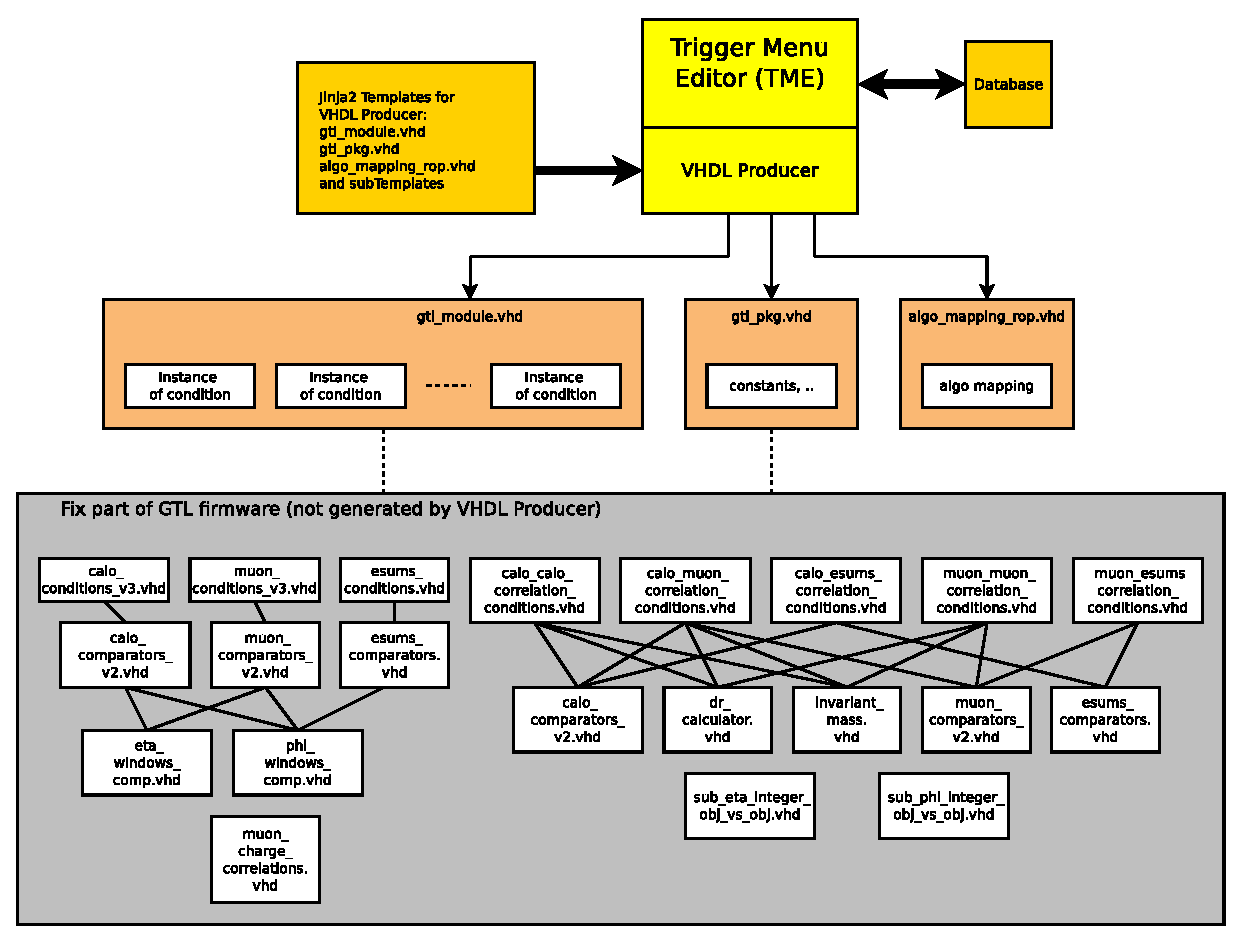
\includegraphics[width=15cm]{figures/tme_gtl}
\caption{VHDL file generation by VHDL Producer} 
\label{fig:gtl:tme_gtl}
\end{figure}

The latency of \ugtl is fixed to 5 bunch crossings,
2 bunch crossings for the pipeline of $\pm$2bx data (for data with +2bx and +1bx), 2 bunch crossings for conditions (fixed), also for the conditions requested in the future,
1 bunch crossing for the logic of Algorithms (See Figure \ref{fig:gtl:gtl_pipeline}).\\

If there are not enough firmware resources in FPGA of one AMC board for 512 Algorithms, more boards could be used. Therefore the 512 Algorithms are \textbf{partitioned by TME} (\eg the first board covers
Algorithms 0..200 and the second Algorithms 201..511). Trigger Menu Editor (TME) will give the number of Algorithms per module as constant in the package module \texttt{gtl\_pkg.vhd}.
This means \ugtl and \ufdl firmware considered as a unit for synthesis.\\

\subsubsection{Top-of-hierarchy module}
\label{sec:gtl:top_module}

The top-of-hierarchy module (\texttt{gtl\_module.vhd}) contains 
\begin {itemize}
\item the pipeline for $\pm$2bx data
\item the instantiations of charge correlation logic of muons (generated by VHDL Producer)
\item the instantiations of calculators for differences in $\eta$ and $\varphi$ (generated by VHDL Producer)
\item the instantiations of conditions (generated by VHDL Producer)
\item a boolean logic for Algorithms (generated by VHDL Producer)
\end {itemize}

Listing~\ref{lst:gtl_module_vhd} contains the entity-declaration of the top-of-hierarchy file (\texttt{gtl\_module.vhd}).

%% "automatic generation" of entity-list (see /scripts/extract_entities.sh)
\lstinputlisting[label=lst:gtl_module_vhd,language=VHDL,caption=Entity declaration of \texttt{gtl\_module.vhd}]{interfaces/gtl_module_tpl.vhd}

\subsubsection{Package module}
\label{sec:gtl:package_module}

All the declarations for arrays ('type'), parameters ('constant') and look-up-tables ('constant') used in modules are in \texttt{gtl\_pkg.vhd} package-file.

\clearpage

\subsection{\ugtl structure}
\label{sec:gtl:mgtl_structure}

\subsubsection{Data $\pm$2bx}
\label{sec:gtl:data_p_m_2bx}

The \ugtl input data flow through a register pipeline of four stages. With those data it is possible to have conditions with objects from
different bunch crossings (within $\pm$2 bunch crossings), \eg for Correlation conditions.\\
See Figure \ref{fig:gtl:gtl_pipeline} for a scheme of \ugtl pipeline structure. The data "data\_p\_1bx" and "data\_p\_2bx" occur 1 respectively 2 bunch crossings
after data for a certain bunch crossing, therefore we got 2 bunch crossings of latency from those data. The data "data\_m\_1bx" and "data\_m\_2bx" have no influence
on latency, because coming before data for a certain bunch crossing.

\begin{figure}[htb]
\centering
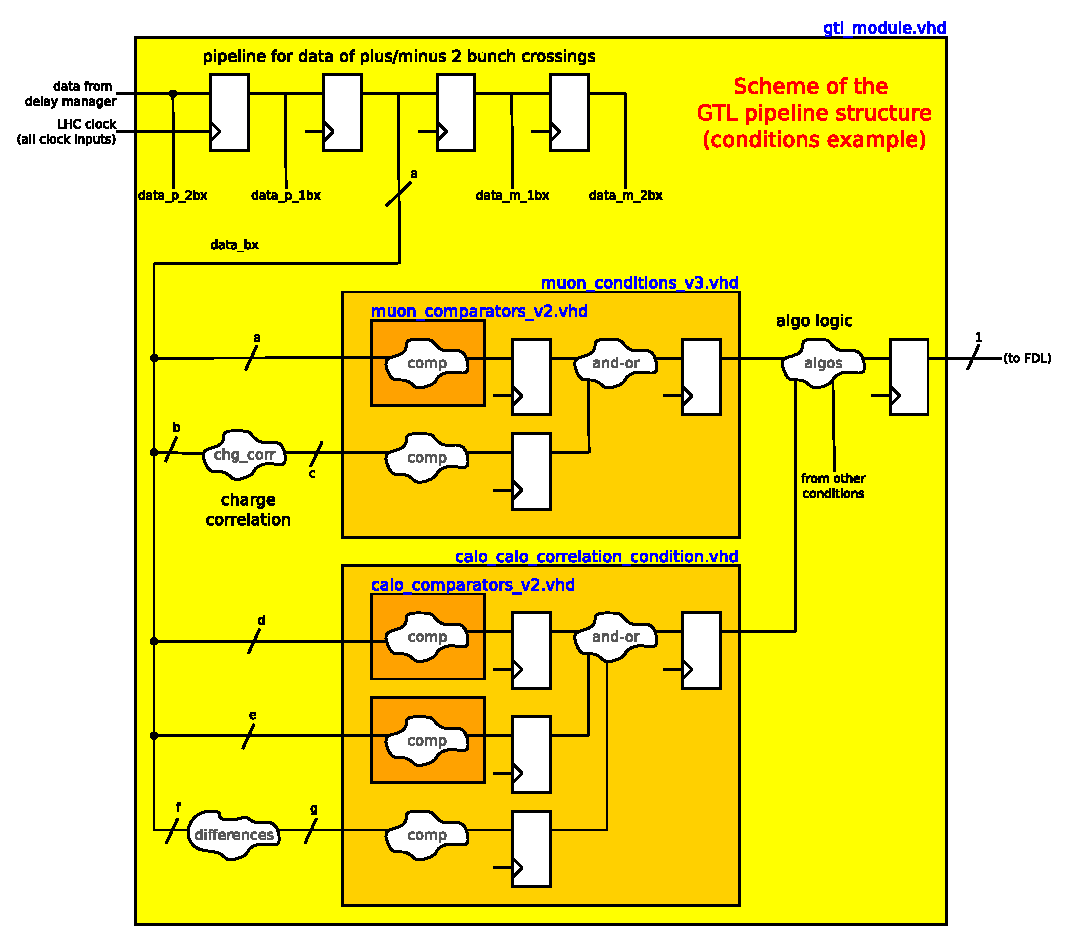
\includegraphics[width=15cm]{figures/gtl_pipeline}
\caption{Scheme of \ugtl pipeline structure} 
\label{fig:gtl:gtl_pipeline}
\end{figure}

\subsubsection{Calculation of differences in $\eta$ and $\varphi$}
\label{sec:gtl:calculation_differences}

Some condition types namely correlation conditions uses differences in $\eta$ and $\varphi$ to make the decision.
Therefore these differences are calculated out of these conditions, because the differences can be used several times in different condition types.
The differences in $\eta$ and $\varphi$ are calculated in bins. These differences in bins are converted to numbers (by LUTs),
which represents values of differences (multiples of units in $\eta$ and $\varphi$).
Differences in $\varphi$ are provided by module \texttt{sub\_phi\_integer\_obj\_vs\_obj.vhd}, which instantiates the module \texttt{sub\_unsigned\_phi.vhd} as many times as
the numbers of both objects determine.\\
In the module \texttt{sub\_unsigned\_phi.vhd} a calculation of a difference of two objects is done, both objects must have the same resolution, namely the higher one.
The result is the absolute value of the difference.
There are two differences in $\varphi$, one "clockwise" and one "anti-clockwise". For the final result the smaller difference is taken.\\
Differences in $\eta$ are provided by module \texttt{sub\_eta\_integer\_obj\_vs\_obj.vhd}, which instantiates the module \texttt{sub\_signed\_eta.vhd} as many times as
the numbers of both objects determine.\\
In the module \texttt{sub\_signed\_eta.vhd} a calculation of a difference of two objects is done with a signed subtraction, because of the Two's Complement notation of $\eta$ values.
The result is the absolute value of the difference. 

\subsubsection{Calorimeter conditions}
\label{sec:gtl:calorimeter_conditions}

\paragraph{Calorimeter data}
\label{sec:gtl:calorimeter_data}

The calorimeter trigger processing identifies \textbf{\egamma, jet and tau} objects and \textbf{\esums}.\\

\textbf{\egamma}:\\ Twelve objects are passed to the \ugt for each event.\\
For each selected object, the Calo-Layer2 sends parameters for \et and for position and quality information - encoded in 32 bits: 
\begin{itemize}
\item 9 bits \et, range = 0..255 GeV (HW index = 0..0x1FF), step = 0.5, the highest bin will mark an overflow (HW index 0x1FF): meaning has to be defined
\item 8 (7+1 sign) bits pseudo-rapidity ($\eta$) position, range = -3.0 to 3.0, step = 0.087/2, linear scale, 138 bins (HW index = 0xBC..0x44)
\item 8 bits azimuth angle ($\varphi$) position, range = 2$\pi$, step $\approx$ 2$\pi$/144 (\^=2.5°), 144 bins (HW index = 0..0x8F), HW index starting at 0° (anti-clockwise)
\item 2 bits isolation (meaning not defined yet!) 
\item 5 bits quality and spare (not defined yet!)
\end{itemize}

The data structure of an \egamma object (bits 27..31 are not defined yet, reserved for quality, ...):
\begin{center}
\begin{bytefield}[boxformatting={\centering\itshape}, bitwidth=1.2em, endianness=big]{32}
        \bitheader{0,8,9,16,17,24,25,26,27,31} \\
        \bitbox {5}     {\texttt{qual/spare}} &
        \bitbox {2}     {\texttt{iso}} &
        \bitbox {8}     {\texttt{$\varphi$}}  &
        \bitbox {8}     {\texttt{$\eta$}}  &
        \bitbox {9}     {\texttt{\et}} \\
\end{bytefield}
\end{center}

\textbf{jet}:\\ Twelve objects are passed to the \ugt for each event.\\
For each selected object, the Calo-Layer2 sends parameters: \et, for position and quality information - encoded in 32 bits: 
\begin{itemize}
\item 11 bits \et, range = 0..1023 GeV (HW index = 0..0x7FF), step = 0.5, the highest bin will mark an overflow (HW index 0x7FF): meaning has to be defined
\item 8 (7+1 sign) bits pseudo-rapidity ($\eta$) position, range = -5.0 to 5.0, step = 0.087/2, linear scale, 230 bins (HW index = 0x8E..0x72)
\item 8 bits azimuth angle ($\varphi$) position, range = 2$\pi$, step $\approx$ 2$\pi$/144 (\^=2.5°), 144 bins (HW index = 0..0x8F), HW index starting at 0° (anti-clockwise)
\item 5 bits quality and spare (not defined yet!)
\end{itemize}

The data structure of a jet object (bits 27..31 are not defined yet, reserved for quality, ...):
\begin{center}
\begin{bytefield}[boxformatting={\centering\itshape}, bitwidth=1.2em, endianness=big]{32}
        \bitheader{0,10,11,18,19,26,27,31} \\
        \bitbox {5}     {\texttt{iso/qu/sp}} &
        \bitbox {8}     {\texttt{$\varphi$}}  &
        \bitbox {8}     {\texttt{$\eta$}}  &
        \bitbox {11}    {\texttt{\et}} \\
\end{bytefield}
\end{center}

\textbf{tau}:\\ Twelve objects are passed to the \ugt for each event.\\
For each selected object, the Calo-Layer2 sends parameters for \et and for position and quality information - encoded in 32 bits: 
\begin{itemize}
\item 9 bits \et, range = 0..255 GeV (HW index = 0..0x1FF), step = 0.5, the highest bin will mark an overflow (HW index 0x1FF): meaning has to be defined
\item 8 (7+1 sign) bits pseudo-rapidity ($\eta$) position, range = -3.0 to 3.0, step = 0.087/2, linear scale, 138 bins (HW index = 0xBC..0x44)
\item 8 bits azimuth angle ($\varphi$) position, range = 2$\pi$, step $\approx$ 2$\pi$/144 (\^=2.5°), 144 bins (HW index = 0..0x8F), HW index starting at 0° (anti-clockwise)
\item 2 bits isolation (meaning not defined yet!) 
\item 5 bits quality and spare (not defined yet!)
\end{itemize}

The data structure of a tau object (bits 27..31 are not defined yet, reserved for quality, ...):
\begin{center}
\begin{bytefield}[boxformatting={\centering\itshape}, bitwidth=1.2em, endianness=big]{32}
        \bitheader{0,8,9,16,17,24,25,26,27,31} \\
        \bitbox {5}     {\texttt{qual/spare}} &
        \bitbox {2}     {\texttt{iso}} &
        \bitbox {8}     {\texttt{$\varphi$}}  &
        \bitbox {8}     {\texttt{$\eta$}}  &
        \bitbox {9}     {\texttt{\et}} \\
\end{bytefield}
\end{center}

The representation of the 8 bits (called "hardware index [HW index]") in $\eta$ is expected as Two's Complement notation as shown in Table~\ref{tab:gtl:calo_eta_scale}.\\
 
\begin{table}[htdp]
\caption{$\eta$ scale of \egamma and tau}
\begin{center}
\begin{tabular}{|c|l|c|}\hline
\textbf{HW index}& \textbf{$\eta$ range} & \textbf{$\eta$ bin}\\\hline\hline
0x44 & 68$*$0.087/2 to 69$*$0.087/2 & 68\\\hline
... & ... & ...\\\hline
0x01 & 0.087/2 to 2$*$0.087/2 & 1\\\hline
0x00 & 0 to 0.087/2 & 0\\\hline
0xFF & 0 to -0.087/2 & -1\\\hline
0xFE & -0.087/2 to -2$*$0.087/2 & -2\\\hline
... & ... & ...\\\hline
0xBC & -68$*$0.087/2 to -69$*$0.087/2 & -69\\\hline
\end{tabular}
\end{center}
\label{tab:gtl:calo_eta_scale}
\end{table}

\begin{table}[htdp]
\caption{$\eta$ scale of jet}
\begin{center}
\begin{tabular}{|c|l|c|}\hline
\textbf{HW index}& \textbf{$\eta$ range} & \textbf{$\eta$ bin}\\\hline\hline
0x72 & 114$*$0.087/2 to 115$*$0.087/2 & 114\\\hline
... & ... & ...\\\hline
0x01 & 0.087/2 to 2$*$0.087/2 & 1\\\hline
0x00 & 0 to 0.087/2 & 0\\\hline
0xFF & 0 to -0.087/2 & -1\\\hline
0xFE & -0.087/2 to -2$*$0.087/2 & -2\\\hline
... & ... & ...\\\hline
0x8E & -114$*$0.087/2 to -115$*$0.087/2 & -115\\\hline
\end{tabular}
\end{center}
\label{tab:gtl:calo_eta_scale}
\end{table}

The representation of the 8 bits in $\varphi$ is expected as shown in Table~\ref{tab:gtl:calo_phi_scale}.\\
 
\begin{table}[htdp]
\begin{center}
\begin{tabular}{|c|l|l|c|}\hline
HW index & $\varphi$ range & $\varphi$ range [degrees] & $\varphi$ bin\\\hline\hline
0x00 & 0 to 2$\pi$/144 & 0 to 2.5 & 0\\\hline
0x01 & 2$\pi$/144 to 2$*$2$\pi$/144 & 2.5 to 5.0 & 1\\\hline
... & ... & ... & ...\\\hline
0x8F & 143$*$2$\pi$/144 to 2$\pi$ & 357.5 to 360 & 143\\\hline
\end{tabular}
\end{center}
\caption{$\varphi$ scale of calorimeter objects}
\label{tab:gtl:calo_phi_scale}
\end{table}

The representation of the 2 bits for isolation (e/$\gamma$ and tau) is expected as shown in Table~\ref{tab:gtl:eg_tau_iso_bits}.\\

\begin{table}[ht]
\caption{Definition of e/$\gamma$ and tau isolation bits}
\vspace{5mm}
\centering
\begin{tabular}{|c|c|}\hline
bits [26..25] & definition \\\hline\hline
00 & not isolated \\
01 & isolated \\
10 & TBD \\
11 & TBD \\\hline
\end{tabular}
\label{tab:gtl:eg_tau_iso_bits}
\end{table}

\clearpage

\paragraph{Calorimeter conditions definition}\label{sec:gtl:calo_cond_def}

A condition consists of calorimeter objects as input data and a set of requirements, which contain the requirements to be complied.

The requirement for calorimeter conditions contains:\\
one threshold for \et, ranges for $\eta$, $\varphi$ LUTs for isolation and differences in $\eta$ and $\varphi$. In addition the selection of the "relative bx" of objects
is done in the requirement.\\
The condition is complied, if every comparison between object parameters and requirements is valid for the following equation:
\begin{itemize}
\item \et greater-equal or equal threshold
\item $\eta$ in range
\item $\varphi$ in range
\item isolation as requested (for \egamma and tau)
\end{itemize}
\textit{Additional comparisons for "quality information" could be part of the equation - but not defined yet.}

There are different types of calorimeter conditions implemented, depending of how many objects have to comply the requirements.
\begin{itemize}
%\item "Quad objects condition", at least four objects have to comply the equation at least with one, but different of four templates.
\item "Quad objects requirements condition": this condition type consists of requirements for 4 different trigger objects of the same object type. 
For each object the requirements can be different. To fulfill this condition, there must exist at least one set of 4 different objects,
each of which fulfills at least one of the requirements.
%\item "Triple objects condition", at least three objects have to comply the equation at least with one, but different of three templates.
\item "Triple objects requirements condition": this condition type consists of requirements for 3 different trigger objects of the same object type. 
For each object the requirements can be different. To fulfill this condition, there must exist at least one set of 3 different objects,
each of which fulfills at least one of the requirements.
%\item "Double objects condition", at least two objects have to comply the equation at least with one, but different of two templates.
\item "Double objects requirements condition": this condition type consists of requirements for 2 different trigger objects of the same object type. 
For each object the requirements can be different. To fulfill this condition, there must exist at least one set of 2 different objects,
each of which fulfills at least one of the requirements.\footnote{"Double objects requirements condition with spatial correlation" not used anymore, replaced by Correlation conditions}
%\item "Double objects condition with spatial correlation", at least two objects have to comply the equation at least with one, but different of two templates. In addition the
%correlation in $\eta$ and $\varphi$ of two objects must be complied.
% \item "Double objects requirements condition with spatial correlation": this condition type consists of requirements for 2 different trigger objects of the same object type. 
% For each object the requirements can be different. To fulfill this condition, there must exist at least one set of 2 different objects,
% each of which fulfills at least one of the requirements. In addition the correlation in $\eta$ and $\varphi$ of two objects must be complied.
%\item "Single object condition", at least one object has to comply the equation with one template.
\item "Single object requirement condition": this condition type consists of one requirement for one trigger object of a given object type. 
To fulfill this condition, there must exist at least one object which fulfills the requirement.

\end{itemize}

% The "double objects requirements condition with spatial correlation" additionally has comparisons for difference of $\eta$ and $\varphi$ (not used anymore in the future, replaced by Correlation conditions).
% Both differences have to be in the range selected with requirements.\\
The selection of the mode of \et-comparator (greater/equal or equal), the \et-threshold-value, ranges for $\eta$ and $\varphi$ set with thresholds, LUTs for isolation and ranges for differences in $\eta$ and $\varphi$ set with thresholds are fixed values given by VHDL Producer for every Trigger Menu.
The objects have to be of same type and same bunch-crossing.

\subparagraph{Calorimeter conditions module}\label{sec:gtl:calo_conditions_module}

The module for conditions with calorimeter objects (\texttt{calo\_conditions.vhd}) instantiates the calorimeter comparators module (\texttt{calo\_comparators.vhd}) as many times as
the numbers of objects and requirements determine. Depending on the condition-type, different and-or-structures of object vs. requirement are selected.
The selection of condition-type and the number of objects is done by parameters in the generic interface list of the module (see Listing~\ref{lst:calo_conditions_vhd},
see also the explanations below).\\
For comparison in $\eta$, $\varphi$ and the differences in $\eta$ and $\varphi$, "window"-comparators are used.\\
In the calorimeter conditions module a cut for two-body pt calculation can be selected (see ~\ref{sec:gtl:twobody_pt_calculation}). Therefore a threshold value for two-body pt is required.\\

%% "automatic generation" of listings (see /scripts/extract_entities.sh)
\lstinputlisting[label=lst:calo_conditions_vhd,language=VHDL,caption=Entity declaration of \texttt{calo\_conditions.vhd}]{interfaces/calo_conditions.vhd}

\medskip
\begin{table}[htdp]
\footnotesize
\begin{center}
\begin{tabular}{l p{.65\columnwidth}}
\toprule
{Item} & {Explanation}\\
\midrule       
\verb|calo_object_slice_1_low| & low value of slice for object 1.\\
\verb|calo_object_slice_1_high| & high value of slice for object 1.\\
\verb|calo_object_slice_2_low| & low value of slice for object 2.\\
\verb|calo_object_slice_2_high| & high value of slice for object 2.\\
\verb|calo_object_slice_3_low| & low value of slice for object 3.\\
\verb|calo_object_slice_3_high| & high value of slice for object 3.\\
\verb|calo_object_slice_4_low| & low value of slice for object 4.\\
\verb|calo_object_slice_4_high| & high value of slice for object 4.\\
\verb|nr_templates| & valid values are 1 (for single), 2 (double), 3 (triple) and 4 (quad) - depending on condition type.\\
\verb|et_ge_mode| & 'mode-selection' for the \et comparator. Valid strings are 'true' and 'false' (type is boolean), 'true' means comparator works on greater/equal, 'false' means equal (for tests only)\\
\verb|obj_type| & valid strings are 'EG\_TYPE', 'JET\_TYPE', and 'TAU\_TYPE'.\\
\verb|et_thresholds| & array of four threshold values for comparison in \et (four thresholds, because of max. 4 requirements).\\
\verb|nr_eta_windows| & array of four integer values for number of $\eta$ cuts.\\
\verb|eta_w1_upper_limits| & array of four "upper limits" of "window"-comparator 1 for $\eta$.\\
\verb|eta_w1_lower_limits| & array of four "lower limits" of "window"-comparator 1 for $\eta$.\\
\verb|eta_w2_upper_limits| & array of four "upper limits" of "window"-comparator 2 for $\eta$.\\
\verb|eta_w2_lower_limits| & array of four "lower limits" of "window"-comparator 2 for $\eta$.\\
\verb|eta_w3_upper_limits| & array of four "upper limits" of "window"-comparator 3 for $\eta$.\\
\verb|eta_w3_lower_limits| & array of four "lower limits" of "window"-comparator 3 for $\eta$.\\
\verb|eta_w4_upper_limits| & array of four "upper limits" of "window"-comparator 4 for $\eta$.\\
\verb|eta_w4_lower_limits| & array of four "lower limits" of "window"-comparator 4 for $\eta$.\\
\verb|eta_w5_upper_limits| & array of four "upper limits" of "window"-comparator 5 for $\eta$.\\
\verb|eta_w5_lower_limits| & array of four "lower limits" of "window"-comparator 5 for $\eta$.\\
\verb|phi_full_range| & array of four boolean to set full range of $\varphi$.\\
\verb|phi_w1_upper_limits| & array of four "upper limits" of "window"-comparator 1 for $\varphi$.\\
\verb|phi_w1_lower_limits| & array of four "lower limits" of "window"-comparator 1 for $\varphi$.\\
\verb|phi_w2_ignore| & array of four boolean to ignore "window"-comparator 2 for $\varphi$.\\
\verb|phi_w2_upper_limits| & array of four "upper limits" of "window"-comparator 2 for $\varphi$.\\
\verb|phi_w2_lower_limits| & array of four "lower limits" of "window"-comparator 2 for $\varphi$.\\
\verb|iso_luts| &  array of four LUTs for comparison of isolation.\\
\verb|twobody_pt_cut| & valid strings are 'true' and 'false' (type is boolean).\\
\verb|pt_width| & vector length of pt value for two-body pt.\\
\verb|pt_sq_threshold_vector| & hex value for threshold of two-body pt comparison (value for pt square).\\
\verb|sin_cos_width| & vector length of sine and cosine.\\
\verb|pt_sq_sin_cos_precision| & precision of sine and cosine calculation in LUTs.\\
\verb|clk| & clock input (LHC clock).\\
\verb|data_i| & data, structure defined in \texttt{obj\_type}.\\
\verb|condition_o| & output of condition (routed to Algorithms logic, see \ref{sec:gtl:algorithms_logic}).\\
\verb|pt| & pt value for two-body pt.\\
\verb|cos_phi_integer| & interger value of cosine for two-body pt.\\
\verb|sin_phi_integer| & interger value of sine for two-body pt.\\
\bottomrule
\end{tabular}
\end{center}
\caption{Explanation of Listing~\ref{lst:calo_conditions_vhd}}
\label{tab:gtl:explanation_calo_conditions_vhd}
\end{table}

\clearpage

\subparagraph{Calorimeter Overlap Remover conditions module}\label{sec:gtl:calo_conditions_orm_module}
The Calorimeter Overlap Remover conditions consits of a Calorimeter condition (\ref{sec:gtl:calo_conditions_module}) and a single condition for a different calo object type. One or more correlation cut(s) ($\Delta\eta$, $\Delta\varphi$ and $\Delta$$R$ - \ref{sec:gtl:correlation_conditions}) for overlap removal is required between different calo object types.
Overlap Remover conditions \texttt{calo\_conditions\_orm.vhd} are implemented only for calo object types.

\subparagraph{Calorimeter conditions module - template for VHDL-Producer}
See in Chapter \ref{sec:gtl:calo_conditions_tme} and in Listing~\ref{lst:instance_calo_condition_vhd} for a VHDL-template for VHDL-Producer of
instantiating a calorimeter condition (\texttt{calo\_conditions.vhd}).\\

\subparagraph{Calorimeter comparators module}\label{sec:gtl:calo_comp_module}
A comparator between the energy (\et) and a threshold (et\_threshold) and a comparison in $\eta$ with five "window"-comparators and $\varphi$ with two "window"-comparators
is done in this basic module. The values for \et threshold, the 'mode-selection' for the \et comparator and the "limits" of the "window"-comparators 
is given in the generic interface list of the module. Additionally the data-structure of input data (data\_i in port interface list) is provided
as a record in this list. The output signal of the module is in high state, if all comparisons are true.\\
The comparison in $\eta$ is done with five "window"-comparators, so one gets max. five ranges for $\eta$. The $\eta$ value (HW index) has a Two's Complement notation, the comparisons is done signed. Number of windows is given for $\eta$.\\
The comparison in $\varphi$ is done with two "window"-comparators, so one gets two ranges for $\varphi$. The comparisons is done unsigned. There are two flags, one for "full-range" and one for "ignore-second-window" for the selection of the ranges.\\
There are two cases how the limits of one "window"-comparator could be set (see also Figure~\ref{fig:gtl:phi_windows_comparator} and Listing~\ref{lst:phi_window_comparator_vhd}):
\begin{itemize}
\item Upper limit is less than lower limit => $\varphi$ range between the limits, including the $\varphi$ bin with value = 0 (HW index).
\item Upper limit is greater/equal than lower limit => $\varphi$ range between the limits, not including the $\varphi$ bin with value = 0 (HW index).
\end{itemize}
The comparison of isolation (for \egamma and tau) is done with LUTs.
\begin{lstlisting}[label=lst:phi_window_comparator_vhd,float=here,caption=VHDL code of "window"-comparator in $\varphi$,captionpos=t]
    phi_comp_w1 <= '1' when phi_w1_upper_limit < phi_w1_lower_limit and
                    (phi <= phi_w1_upper_limit or phi >= phi_w1_lower_limit) else
                   '1' when phi_w1_upper_limit >= phi_w1_lower_limit and
                    (phi <= phi_w1_upper_limit and phi >= phi_w1_lower_limit)
                    else '0';
\end{lstlisting}

The values of $\eta$ and $\varphi$ have to be inside of only one of the required ranges ("or").

The comparison of isolation (for \egamma and tau) is done with LUTs (see Table~\ref{tab:gtl:calo_lut_iso}).
Only the least significant 4 bits of LUT are used, because currently 2 isolation bits are defined. 

\begin{table}[htdp]
\begin{center}
\begin{tabular}{|c|c|p{.4\columnwidth}|}\hline
LUT content (16 bits) & isolation bits [26..25] & trigger \\\hline\hline
X"0" & xx & no trigger\\\hline
X"1" & 00 & trigger on isolation bits = 00\\\hline
X"2" & 01 & trigger on isolation bits = 01\\\hline
X"3" & 00 or 01 & trigger on isolation bits = 00 or 01\\\hline
X"4" & 10 & trigger on isolation bits = 10\\\hline
X"5" & 00 or 10 & trigger on isolation bits = 00 or 10\\\hline
X"6" & 01 or 10 & trigger on isolation bits = 01 or 10\\\hline
X"7" & 00 or 01 or 10 & trigger on isolation bits = 00 or 01 or 10\\\hline
X"8" & 11 & trigger on isolation bits = 11\\\hline
X"9" & 00 or 11 & trigger on isolation bits = 00 or 11\\\hline
X"A" & 01 or 11 & trigger on isolation bits = 01 or 11\\\hline
X"B" & 00 or 01 or 11 & trigger on isolation bits = 00 or 01 or 11\\\hline
X"C" & 10 or 11 & trigger on isolation bits = 10 or 11\\\hline
X"D" & 00 or 10 or 11 & trigger on isolation bits = 00 or 10 or 11\\\hline
X"E" & 01 or 10 or 11 & trigger on isolation bits = 01 or 10 or 11\\\hline
X"F" & 00 or 01 or 10 or 11 & trigger on isolation bits = 00 or 01 or 10 or 11 (= "ignore" isolation)\\\hline
\end{tabular}
\end{center}
\caption{LUT contents for isolation comparison of \egamma and tau objects}
\label{tab:gtl:calo_lut_iso}
\end{table}

\begin{figure}[htb]
\centering
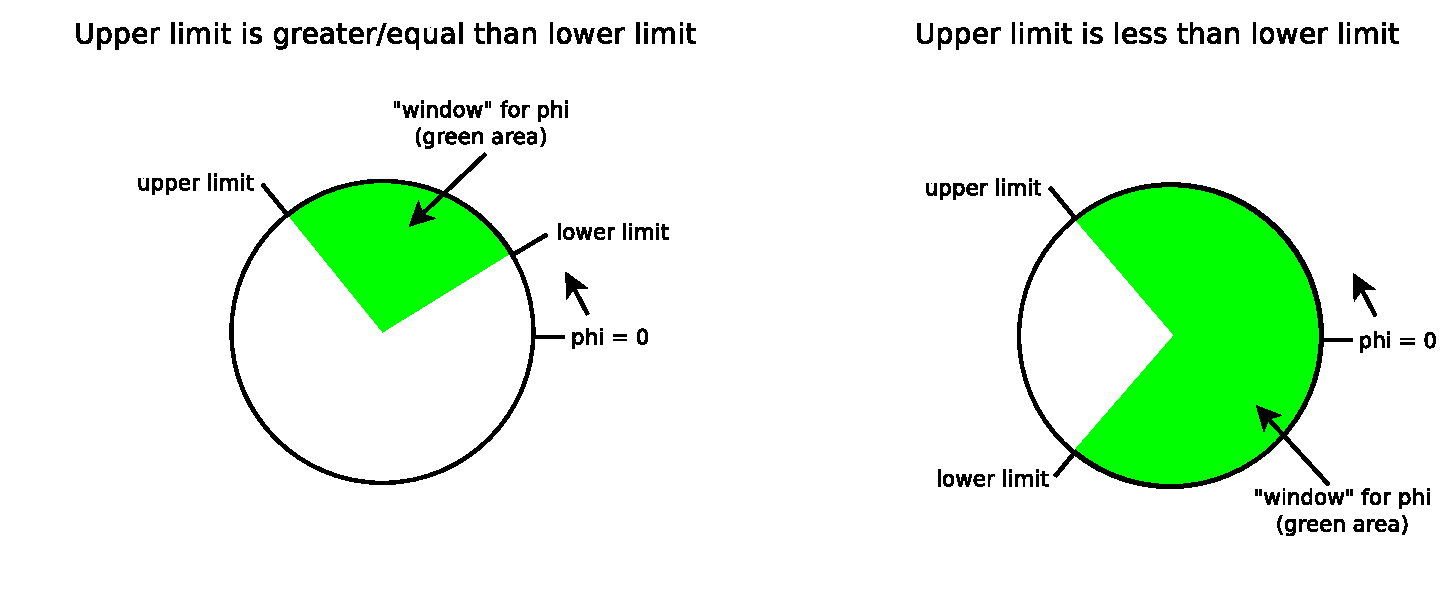
\includegraphics[width=15cm]{figures/phi_windows_comparator}
\caption{Setting the limits for "window"-comparators for $\varphi$} 
\label{fig:gtl:phi_windows_comparator}
\end{figure}

\clearpage

\subsubsection{Energy sum quantities conditions}
\label{sec:gtl:esums_conditions}

\textbf{\esums}:\\ Consists of following quantities (naming convention see \ref{sec:glossary}):
\begin{itemize}
\item \textbf{\ett}
\item \textbf{\htt}
\item \textbf{\etm}
\item \textbf{\htm}
\item \textbf{ETTEM}
\item \textbf{ET$_{miss}^{HF}$}
\item \textbf{HT$_{miss}^{HF}$}
\item \textbf{ASYMET}
\item \textbf{ASYMHT}
\item \textbf{ASYMETHF}
\item \textbf{ASYMHTHF}
\item \textbf{CENT0}
\item \textbf..
\item \textbf{CENT7}
\end{itemize}

\paragraph{Energy sum quantities data}
Calo-Layer2 sends 6 frames (each 32 bits) with Energy sum quantities containing the following information:
\begin{itemize}
\item \et, 12 bits, range = 0..2047 GeV (HW index = 0..0xFFF), step = 0.5, the highest bin will mark an overflow (HW index 0xFFF): meaning has to be defined
\item azimuth angle ($\varphi$) position, 8 bits, range = 2$\pi$, step $\approx$ 2$\pi$/144 (\^=2.5°), 144 bins (HW index = 0..0x8F), HW index starting at 0° (anti-clockwise)
\item "Towercount", 13 bits, range = 0..8191
\item "Minimum bias", 4 bits, range = 0..15
\item "Asymmetry", 8 bits, range = 0..255 (used 0..100)
\item "Centrality", 8 bits, used as signals
\end{itemize}

Frame0: The data structure of "total Et" (\ett) quantity [including "total Et from ECAL only" (ETTEM) and "minimum bias HF+ threshold 0" bits]:
\begin{center}
\begin{bytefield}[boxformatting={\centering\itshape}, bitwidth=1.2em, endianness=big]{32}
        \bitheader{0,11,12,23,24,27,28,31} \\
        \bitbox {4}    {\texttt{MBT0HFP}} &
        \bitbox {4}    {\texttt{spare}} &
        \bitbox {12}    {\texttt{\et [ETTEM]}} &
        \bitbox {12}    {\texttt{\et [\ett]}} \\
\end{bytefield}
\end{center}

Frame1: The data structure of "total calibrated Et in jets" (\htt) quantity [including "towercount" and "minimum bias HF- threshold 0" bits]:
\begin{center}
\begin{bytefield}[boxformatting={\centering\itshape}, bitwidth=1.2em, endianness=big]{32}
        \bitheader{0,11,12,24,25,27,28,31} \\
        \bitbox {4}    {\texttt{MBT0HFM}} &
        \bitbox {3}    {\texttt{spare}} &
        \bitbox {13}    {\texttt{TOWERCOUNT}} &
        \bitbox {12}    {\texttt{\et}} \\
\end{bytefield}
\end{center}

Frame2: The data structure of "missing Et" (\etm) quantity [including "Asymmetry" ASYMET and "minimum bias HF+ threshold 1" bits]:
\begin{center}
\begin{bytefield}[boxformatting={\centering\itshape}, bitwidth=1.2em, endianness=big]{32}
        \bitheader{0,11,12,19,20,27,28,31} \\
        \bitbox {4}    {\texttt{MBT1HFP}} &
        \bitbox {8}    {\texttt{ASYMET}} &
        \bitbox {8}     {\texttt{$\varphi$}} &
        \bitbox {12}    {\texttt{\et}} \\
\end{bytefield}
\end{center}

Frame3: The data structure of "missing Ht" (\htm) quantity [including "Asymmetry" ASYMHT and "minimum bias HF- threshold 1" bits]:
\begin{center}
\begin{bytefield}[boxformatting={\centering\itshape}, bitwidth=1.2em, endianness=big]{32}
        \bitheader{0,11,12,19,20,27,28,31} \\
        \bitbox {4}    {\texttt{MBT1HFM}} &
        \bitbox {8}    {\texttt{ASYMHT}} &
        \bitbox {8}     {\texttt{$\varphi$}} &
        \bitbox {12}    {\texttt{\et}} \\
\end{bytefield}
\end{center}

Frame4: The data structure of "missing Et including HF" (ET$_{miss}^{HF}$) quantity [including "Asymmetry" ASYMETHF and "Centrality" bits (3:0)]:
\begin{center}
\begin{bytefield}[boxformatting={\centering\itshape}, bitwidth=1.2em, endianness=big]{32}
        \bitheader{0,11,12,19,20,27,28,31} \\
        \bitbox {4}    {\small \texttt{CENT[3:0]}} &
        \bitbox {8}    {\texttt{ASYMETHF}} &
        \bitbox {8}     {\texttt{$\varphi$}} &
        \bitbox {12}    {\texttt{\et}} \\
\end{bytefield}
\end{center}

Frame5: The data structure of "missing Ht including HF" (HT$_{miss}^{HF}$) quantity [including "Asymmetry" ASYMHTHF and "Centrality" bits (7:4)]:
\begin{center}
\begin{bytefield}[boxformatting={\centering\itshape}, bitwidth=1.2em, endianness=big]{32}
        \bitheader{0,11,12,19,20,27,28,31} \\
        \bitbox {4}    {\small \texttt{CENT[7:4]}} &
        \bitbox {8}    {\texttt{ASYMHTHF}} &
        \bitbox {8}     {\texttt{$\varphi$}} &
        \bitbox {12}    {\texttt{\et}} \\
\end{bytefield}
\end{center}

\paragraph{Energy sum quantities conditions module (including Asymmetry conditions)}

For the entity-declaration of \texttt{esums\_conditions.vhd}, see Listing~\ref{lst:esums_conditions_vhd}.

% "automatic generation" of listings (see /scripts/extract_entities.sh)
%% REMARK: HB 2015-04-29: esums_conditions.vhd is not in ../firmware/gt_mp7/trunk/src and (scripts/extract_entities.sh) now, so interfaces/esums_conditions.vhd was copied and edited by hand.
\lstinputlisting[label=lst:esums_conditions_vhd,language=VHDL,caption=Entity declaration of \texttt{esums\_conditions.vhd}]{interfaces/esums_conditions.vhd}

\medskip
\begin{table}[htdp]
\footnotesize
\begin{center}
\begin{tabular}{l p{.7\columnwidth}}
\toprule
{Item} & {Explanation}\\
\midrule       
\verb|et_ge_mode| & 'mode-selection' for the \et comparator. Valid strings are 'true' and 'false' (type is boolean), 'true' means comparator works on greater/equal, 'false' means equal (for tests only)\\
\verb|obj_type| &  valid strings are 'ETT\_TYPE', 'HTT\_TYPE', 'ETM\_TYPE', 'HTM\_TYPE' and 'ETMHF\_TYPE'.\\
\verb|et_threshold| & threshold value for comparison in \et. The size of the std\_logic\_vector depends on the number of \et bits.\\
\verb|phi_full_range| & boolean to set full range of $\varphi$.\\
\verb|phi_w1_upper_limits| & "upper limit" of "window"-comparator 1 for $\varphi$.\\
\verb|phi_w1_lower_limits| & "lower limit" of "window"-comparator 1 for $\varphi$.\\
\verb|phi_w2_ignore| & boolean to ignore "window"-comparator 2 for $\varphi$.\\
\verb|phi_w2_upper_limits| & "upper limit" of "window"-comparator 2 for $\varphi$.\\
\verb|phi_w2_lower_limits| & "lower limit" of "window"-comparator 2 for $\varphi$.\\
\verb|clk| & clock input (LHC clock).\\
\verb|data_i| & input data, structure defined in \texttt{obj\_type}.\\
\verb|condition_o| & output of condition (routed to Algorithms logic, see \ref{sec:gtl:algorithms_logic}).\\
\bottomrule
\end{tabular}
\end{center}
\caption{Explanation of Listing~\ref{lst:esums_conditions_vhd}}
\label{tab:gtl:explanation_esums_conditions_vhd}
\end{table}

A comparator between \et and a threshold (et\_threshold) and, depending on object type, a comparison in $\varphi$ with 
two "window"-comparators is done in this module. 
The value for \et threshold, the 'mode-selection' for the \et comparator and the limits for the "window"-comparators are given in the generic interface list of the module.
The selection whether a comparison in $\varphi$ is part of the condition is done with the value of the generic parameter 'obj\_type' 
('ETM\_TYPE', 'ETMHF\_TYPE', 'HTM\_TYPE' and 'HTMHF\_TYPE' force a comparison).
The comparison in $\varphi$ is done in the same way as for calorimeter conditions (see \ref{sec:gtl:calo_comp_module}).
Additionally the data-structure of input data (data\_i in port interface list) is provided
as a record in this list. The output signal of the module is in high state, if all comparisons are true.\\
Data for Asymmetry trigger are received on 4 frames on bits 27..20 (8 bits). For every type a comparision with an 8-bit threshold (greater-equal or equal) is done.
Asymmetry data are interpreted as counts.

\paragraph{Energy sum quantities conditions module - template for VHDL-Producer}
A VHDL-template for VHDL-Producer of instantiating \texttt{esums\_conditions.vhd} is given below (see Listing~\ref{lst:instance_esums_condition_vhd}).\\

\subsubsection{Minimum bias trigger conditions}
\label{sec:gtl:min_bias_conditions}

Data for Minimum bias trigger are received on the 4 MSBs of 4 frames used for Energy sum quantities (see \ref{sec:gtl:esums_conditions}). 

\begin{itemize}
\item MBT0HFP: "minimum bias HF+ threshold 0" bits
\item MBT0HFM: "minimum bias HF- threshold 0" bits
\item MBT1HFP: "minimum bias HF+ threshold 1" bits
\item MBT1HFM: "minimum bias HF- threshold 1" bits
\end{itemize}

In the min\_bias\_hf\_conditions.vhd module there is a comparision with a 4-bit threshold (greater-equal or equal).

\subsubsection{Towercount condition}
\label{sec:gtl:towercount_cond}

Data for Towercount trigger (number of firing HCAL towers) are received on frame \htt (see \ref{sec:gtl:esums_conditions}) on bits 24..12 (13 bits) of \htt data structure. 
In the towercount\_condition.vhd module there is a comparision with a 13-bit threshold (greater-equal or equal).

\subsubsection{Centrality condition}
\label{sec:gtl:centrality_cond}

Centrality bits used as a signals for triggers (similar to external signals).

\subsubsection{Muon conditions}
\label{sec:gtl:muon_conditions}

\paragraph{Muon data}
\label{sec:gtl:muon_data}
Eight Muon objects are provided by \gmt. One Muon object has a 64 bits data structure with parameters for \pt, for position, charge, quality and isolation information: 
\begin{itemize}
\item 10 bits azimuth angle ($\varphi$) position, range = 2$\pi$, step $\approx$ 2$\pi$/576 (\^=0.625°), 576 bins (HW index = 0..0x23F), HW index starting at 0° (anti-clockwise)
\item 9 bits \pt, range = 0..255 GeV (HW index = 0..0x1FF), step = 0.5, the highest bin will mark an overflow (HW index 0x1FF): meaning has to be defined
\item 4 bits quality, 16 types for quality (meaning not defined yet!)
\item 9 (8+1 sign) bits pseudo-rapidity ($\eta$) position, range = -2.45 to 2.45, step = 0.087/8, linear scale, 452 bins (-225..225, HW index = 0x11F..0x0E1)
\item 2 bits isolation, 4 types for isolation (meaning not defined yet!)
\item 1 bit charge sign, charge sign = '0' means "positive" charge, charge sign = '1' means "negative" charge
\item 1 bit charge valid (='1' means "valid")
\item 7 index bits
\item 10 bits azimuth angle ($\varphi$) position, raw data
\item 8 bits unconstraint \pt, range = 0..255 GeV (HW index = 0..0xFF), step = 1.0, the highest bin will mark an overflow (HW index 0xFF)
\item 1 spare bit
\item 2 bits impact parameter
\end{itemize}

The data structure of a muon object (64 bits - bit 34 = charge sign, bit 35 = charge valid, bit 61 is a spare bit, bit 63..62 = impact parameter):
\begin{center}
\begin{bytefield}[boxformatting={\centering\itshape}, endianness=big, bitwidth=1.2em]{32}
        \bitheader[lsb=32]{32,33,34,35,36,42,43,52,53,60,61,61,62,63} \\
        \bitbox {2}     {\small  \texttt{imp para}}       &
        \bitbox {1}     {\small  \texttt{r}}       &
        \bitbox {8}     {\texttt{unconst.\pt}}       &
        \bitbox {10}    {\texttt{$\varphi$} (out)}
        \bitbox {7}     {\texttt{index bits}}
        \bitbox {2}     {\small  \texttt{ch}}       &
        \bitbox {2}     {\small \texttt{iso}} \\
        [3ex]
        \bitheader{0,9,10,18,19,22,23,31} \\
        \bitbox {9}     {\texttt{$\eta$} (extrapol.)}       &
        \bitbox {4}     {\texttt{qual}}       &
        \bitbox {9}     {\texttt{\pt}}    &
        \bitbox {10}    {\texttt{$\varphi$} (extrapol.)} \\
\end{bytefield}
\end{center}

The representation of the 9 bits (called "hardware index [HW index]") in $\eta$ is expected as Two's Complement notation as shown in Table~\ref{tab:gtl:muon_eta_scale}.\\
The central value of the bin 0 (-0.010875/2 to +0.010875/2) = 0.0, the left edge of the bins will range from $-255 \times 0.010875 - 0.010875/2 = -2.7785625$ to $+255 \times 0.010875 - 0.010875/2 = 2.7676875$.
The central value of the bins will range between $\pm 2.773125$ . The physical $\eta$ range of the muon detectors is about $\pm2.45$, so that not all possible $\eta$ bins will be used.\\ 
 
\begin{table}[htdp]
\begin{center}
\begin{tabular}{|c|l|c|}\hline
HW index & $\eta$ range & $\eta$ bin\\\hline\hline
0x0E1 & 224.5$*$0.087/8 to 225.5$*$0.087/8 & 225\\\hline
0x0E0 & 223.5$*$0.087/8 to 224.5$*$0.087/8 & 224\\\hline
... & ... & ...\\\hline
0x001 & 0.5$*$0.087/8 to 1.5$*$0.087/8 & 1\\\hline
0x000 & 0.5$*$-0.087/8 to 0.5$*$0.087/8 & 0\\\hline
0x1FF & 0.5$*$-0.087/8 to 1.5$*$-0.087/8 & -1\\\hline
0x1FE & 1.5$*$-0.087/8 to -2.5$*$0.087/8 & -2\\\hline
... & ... & ...\\\hline
0x11F & -224.5$*$0.087/8 to -225.5$*$0.087/8 & -225\\\hline
\end{tabular}
\end{center}
\caption{$\eta$ scale of muon objects}
\label{tab:gtl:muon_eta_scale}
\end{table}

The representation of the 10 bits in $\varphi$ is expected as shown in Table~\ref{tab:gtl:muon_phi_scale}.\\
 
\begin{table}[htdp]
\begin{center}
\begin{tabular}{|c|l|l|c|}\hline
HW index & $\varphi$ range & $\varphi$ range [degrees] & $\varphi$ bin\\\hline\hline
0x000 & 0 to 2$\pi$/576 & 0 to 0.625 & 0\\\hline
0x001 & 2$\pi$/576 to 2$*$2$\pi$/576 & 0.625 to 1.250 & 1\\\hline
... & ... & ... & ...\\\hline
0x23F & 575$*$2$\pi$/576 to 2$\pi$ & 359.375 to 360 & 575\\\hline
\end{tabular}
\end{center}
\caption{$\varphi$ scale of muon objects}
\label{tab:gtl:muon_phi_scale}
\end{table}

The representation of the 4 bits for quality is expected as shown in Table~\ref{tab:gtl:muon_quality_bits}.\\
 
\begin{table}[ht]
\caption{Definition of muon quality bits}
\vspace{5mm}
\centering
\begin{tabular}{|c|c|}\hline
bits [22..19] & definition \\\hline\hline
0000 & quality "level 0" \\
0001 & quality "level 1" \\
0010 & quality "level 2" \\
0011 & quality "level 3" \\
0100 & quality "level 4" \\
0101 & quality "level 5" \\
0110 & quality "level 6" \\
0111 & quality "level 7" \\
1000 & quality "level 8" \\
1001 & quality "level 9" \\
1010 & quality "level 10" \\
1011 & quality "level 11" \\
1100 & quality "level 12" \\
1101 & quality "level 13" \\
1110 & quality "level 14" \\
1111 & quality "level 15" \\\hline
\end{tabular}
\label{tab:gtl:muon_quality_bits}
\end{table}

The representation of the 2 bits for isolation is expected as shown in Table~\ref{tab:gtl:muon_iso_bits}.\\
 
\begin{table}[ht]
\caption{Definition of muon isolation bits}
\vspace{5mm}
\centering
\begin{tabular}{|c|c|}\hline
bits [33..32] & definition \\\hline\hline
00 & not isolated \\
01 & isolated \\
10 & TBD \\
11 & TBD \\\hline
\end{tabular}
\label{tab:gtl:muon_iso_bits}
\end{table}

The representation of the 2 bits for impact parameter is expected as shown in Table~\ref{tab:gtl:muon_iso_bits}.\\
 
\begin{table}[ht]
\caption{Definition of muon impact parameter bits}
\vspace{5mm}
\centering
\begin{tabular}{|c|c|}\hline
bits [63..62] & definition \\\hline\hline
00 & TBD \\
01 & TBD \\
10 & TBD \\
11 & TBD \\\hline
\end{tabular}
\label{tab:gtl:muon_iso_bits}
\end{table}

\clearpage

\paragraph{Muon charge correlation module}\label{sec:gtl:muon_charge_correlation_module}

For definition of muon charge, see \ref{sec:gtl:muon_conditions}.\\
In the muon charge correlation module, the charge correlations are made for different muon conditions-types. The module is instantiated in the top-of-hierarchy module (\texttt{gtl\_module.vhd})
and not inside of a muon conditions module. 
The charges of objects (number of objects depends on muon condition type) are compared to get "like sign charge" ("LS") or "opposite sign charge" ("0S"), "LS" means that the charges (charge sign)
of objects are the same, "0S" means that at least one object has different charge than the others. This information is used in all instatiated muon conditions.
There is no charge correlation for single type conditions.\\
In all cases the "charge valid" bit of the objects must be set.\\
In TME one can select "LS", "0S" or ignore for charge correlation in muon conditions.\\

% % Insert as table !!!
% Double Muon
% 
% x x : I ignore (charge x = +, -, I)
% + + : LS both positive muons
% - - : LS both negative muons
% I I : LS both muons with the same sign, positive or negative
% + - : OS two muons of opposite sign
% - + : OS idem
% I I : OS idem
% 
% TripleMuon:
% 
% x x x : I  ignore (charge x = +, -, I)
% + + + : LS three muons of positive charge
% - - - : LS three muons of negative charge
% I I I : LS three muons of the same sign (positive or negative)
% + + - : OS a pair plus a positive muon
% + - - : OS a pair plus a negative muon
% + - I : OS a pair plus a negative or positive muon
% 
% QuadMuon
% 
% x x x x : I  ignore (charge x = +, -, I)
% + + + + : LS four muons of positive charge
% - - - - : LS four muons of negative charge
% I I I I : LS four muons of the same sign (positive or negative)
% + + + - : OS a pair plus two positive muons
% + + - - : OS two pairs
% + - - - : OS a pair plus two negative muons
% + - I I : OS a pair plus two negative or positive muons
% 

\begin{table}[ht]
\caption{Muon charge correlation - Double Muon}
\vspace{5mm}
\centering
\begin{tabular}{|c|l|}\hline
\verb|x x| & I ignore (charge x = +, -, I) \\
\verb|+ +| & LS both positive muons \\
\verb|- -| & LS both negative muons \\
\verb|I I| & LS both muons with the same sign, positive or negative \\
\verb|+ -| & OS two muons of opposite sign \\
\verb|- +| & OS idem \\
\verb|I I| & OS idem \\\hline
\end{tabular}
\label{tab:gtl:muon_charge_corr_double}
\end{table}

\begin{table}[ht]
\caption{Muon charge correlation - Triple Muon}
\vspace{5mm}
\centering
\begin{tabular}{|c|l|}\hline
\verb|x x x| & I  ignore (charge x = +, -, I) \\
\verb|+ + +| & LS three muons of positive charge \\
\verb|- - -| & LS three muons of negative charge \\
\verb|I I I| & LS three muons of the same sign (positive or negative) \\
\verb|+ + -| & OS a pair plus a positive muon \\
\verb|+ - -| & OS a pair plus a negative muon \\
\verb|+ - I| & OS a pair plus a negative or positive muon \\\hline
\end{tabular}
\label{tab:gtl:muon_charge_corr_triple}
\end{table}

\begin{table}[ht]
\caption{Muon charge correlation - Quad Muon}
\vspace{5mm}
\centering
\begin{tabular}{|c|l|}\hline
\verb|x x x x| & I  ignore (charge x = +, -, I) \\
\verb|+ + + +| & LS four muons of positive charge \\
\verb|- - - -| & LS four muons of negative charge \\
\verb|I I I I| & LS four muons of the same sign (positive or negative) \\
\verb|+ + + -| & OS a pair plus two positive muons \\
\verb|+ + - -| & OS two pairs \\
\verb|+ - - -| & OS a pair plus two negative muons \\
\verb|+ - I I| & OS a pair plus two negative or positive muons \\\hline
\end{tabular}
\label{tab:gtl:muon_charge_corr_quad}
\end{table}

\clearpage

\paragraph{Muon conditions definition}\label{sec:gtl:muon_cond_def}

A condition consists of input-data and a set of requirements, which contain the requirements to be complied.

The requirement for muon conditions contains:\\
a threshold for \pt, ranges for $\eta$ and $\varphi$, a LUT for quality, a LUT for isolation, 
a requsted charge.
The condition is complied, if every comparison between object parameters and requirements is valid for the following equation:
\begin{itemize}
\item \pt greater-equal or equal threshold
\item $\eta$ in range
\item $\varphi$ in range
\item requested charge 
\item quality LUT
\item iso LUT
\end{itemize}

There are different types of calorimeter conditions implemented, depending of how many objects have to comply the requirements.
\begin{itemize}
\item "Quad objects requirements condition": this condition type consists of requirements for 4 different trigger objects of the same object type. 
For each object the requirements can be different. To fulfill this condition, there must exist at least one set of 4 different objects,
each of which fulfills at least one of the requirements.
\item "Triple objects requirements condition": this condition type consists of requirements for 3 different trigger objects of the same object type. 
For each object the requirements can be different. To fulfill this condition, there must exist at least one set of 3 different objects,
each of which fulfills at least one of the requirements.
\item "Double objects requirements condition": this condition type consists of requirements for 2 different trigger objects of the same object type. 
For each object the requirements can be different. To fulfill this condition, there must exist at least one set of 2 different objects,
each of which fulfills at least one of the requirements.\footnote{"Double objects requirements condition with spatial correlation" not used anymore, replaced by Correlation conditions}
\item "Single object requirement condition": this condition type consists of one requirement for one trigger object of a given object type. 
To fulfill this condition, there must exist at least one object which fulfills the requirement.

\end{itemize}

In addition requested charge correlation must be matched (except for "Single object requirement condition", there is no charge correlation).
The calculation of charge correlations is done in an own module in the top-of-hierarchy module (\texttt{gtl\_module.vhd}).\\

\subparagraph{Muon conditions module}
A module for conditions with muon objects (\texttt{muon\_conditions.vhd}) instantiates the muon comparators module (\texttt{muon\_comparators.vhd}) as many times as
the numbers of objects and requirements determine. Depending on the condition-type different and-or-structures of object vs. requirement are selected.
The selection of condition-type and the number of objects is done by parameters in the generic interface list of the module
(see the following VHDL entity definition in Listing~\ref{lst:muon_conditions_vhd}).\\

\clearpage
%% "automatic generation" of listings (see /scripts/extract_entities.sh)
\lstinputlisting[label=lst:muon_conditions_vhd,language=VHDL,caption=Entity declaration of \texttt{muon\_conditions.vhd}]{interfaces/muon_conditions.vhd}

\clearpage

\begin{longtable}{>{\footnotesize}l >{\footnotesize}p{.65\columnwidth}}
\caption{Explanation of Listing~\ref{lst:muon_conditions_vhd}}\\
\hline 
{Item} & {Explanation}\\
\hline 
\endhead
\verb|muon_object_slice_1_low| & low value of slice for object 1.\\
\verb|muon_object_slice_1_high| & high value of slice for object 1.\\
\verb|muon_object_slice_2_low| & low value of slice for object 2.\\
\verb|muon_object_slice_2_high| & high value of slice for object 2.\\
\verb|muon_object_slice_3_low| & low value of slice for object 3.\\
\verb|muon_object_slice_3_high| & high value of slice for object 3.\\
\verb|muon_object_slice_4_low| & low value of slice for object 4.\\
\verb|muon_object_slice_4_high| & high value of slice for object 4.\\
\verb|nr_templates| & number of requirements, selector of condition-type. Valid values are 1, 2, 3 and 4.\\
\verb|pt_ge_mode| & 'mode-selection' for the \pt comparator. Valid strings are 'true' and 'false' (type is boolean), 'true' means comparator works on greater/equal, 'false' means equal (for tests only)\\
\verb|pt_thresholds| & array of four threshold values for comparison in pt (four threshold, because of max. 4 requirements).\\
\verb|nr_eta_windows| & array of four integer values for number of $\eta$ cuts.\\
\verb|eta_w1_upper_limits| & array of four "upper limits" of "window"-comparator 1 for $\eta$.\\
\verb|eta_w1_lower_limits| & array of four "lower limits" of "window"-comparator 1 for $\eta$.\\
\verb|eta_w2_upper_limits| & array of four "upper limits" of "window"-comparator 2 for $\eta$.\\
\verb|eta_w2_lower_limits| & array of four "lower limits" of "window"-comparator 2 for $\eta$.\\
\verb|eta_w3_upper_limits| & array of four "upper limits" of "window"-comparator 3 for $\eta$.\\
\verb|eta_w3_lower_limits| & array of four "lower limits" of "window"-comparator 3 for $\eta$.\\
\verb|eta_w4_upper_limits| & array of four "upper limits" of "window"-comparator 4 for $\eta$.\\
\verb|eta_w4_lower_limits| & array of four "lower limits" of "window"-comparator 4 for $\eta$.\\
\verb|eta_w5_upper_limits| & array of four "upper limits" of "window"-comparator 5 for $\eta$.\\
\verb|eta_w5_lower_limits| & array of four "lower limits" of "window"-comparator 5 for $\eta$.\\
\verb|phi_full_range| & array of four boolean to set full range of $\varphi$.\\
\verb|phi_w1_upper_limits| & array of four "upper limits" of "window"-comparator 1 for $\varphi$.\\
\verb|phi_w1_lower_limits| & array of four "lower limits" of "window"-comparator 1 for $\varphi$.\\
\verb|phi_w2_ignore| & array of four boolean to ignore "window"-comparator 2 for $\varphi$.\\
\verb|phi_w2_upper_limits| & array of four "upper limits" of "window"-comparator 2 for $\varphi$.\\
\verb|phi_w2_lower_limits| & array of four "lower limits" of "window"-comparator 2 for $\varphi$.\\
\verb|requested_charges| & array of four strings for requested charge ("pos" means "positive charge", "neg" means "negative charge" and "ign" means "ignore charge").\\
\verb|qual_luts| & array of four LUTs (16 bits) for quality.\\
\verb|iso_luts| & array of four LUTs (4 bits) for isolation.\\
\verb|upt_cuts| & array of four boolean for using unconstraint \pt cuts.\\
\verb|upt_upper_limits| & array of four "upper limits" of unconstraint \pt.\\
\verb|upt_lower_limits| & array of four "lower limits" of unconstraint \pt.\\
\verb|ip_luts| & array of four LUTs (4 bits) for impact parameter.\\
\verb|requested_charge_correlation| & string (2 characters) for requested charge correlation ("ls" means "like sign", "os" means "opposite sign" or "ig" means "ignore").\\
\verb|twobody_pt_cut| & valid strings are 'true' and 'false' (type is boolean).\\
\verb|pt_width| & vector length of pt value for two-body pt.\\
\verb|pt_sq_threshold_vector| & hex value for threshold of two-body pt comparison (value for pt square).\\
\verb|sin_cos_width| & vector length of sine and cosine.\\
\verb|pt_sq_sin_cos_precision| & precision of sine and cosine calculation in LUTs.\\
\verb|lhc_clk| & clock input (LHC clock).\\
\verb|data_i| & input data, structure defined in \texttt{d\_s\_i}.\\
\verb|condition_o| & output of condition (routed to Algorithms logic, see \ref{sec:gtl:algorithms_logic}).\\
\verb|ls_charcorr_double| & array of "like sign" charge correlation for double condition.\\
\verb|os_charcorr_double| & array of "opposite sign" charge correlation for double condition.\\
\verb|ls_charcorr_triple| & array of "like sign" charge correlation for triple condition.\\
\verb|os_charcorr_triple| & array of "opposite sign" charge correlation for triple condition.\\
\verb|ls_charcorr_quad| & array of "like sign" charge correlation for quad condition.\\
\verb|os_charcorr_quad| & array of "opposite sign" charge correlation for quad condition.\\
\verb|pt| & pt value for two-body pt.\\
\verb|cos_phi_integer| & interger value of cosine for two-body pt.\\
\verb|sin_phi_integer| & interger value of sine for two-body pt.\\
\hline 
\label{tab:gtl:explanation_muon_conditions_vhd}
\end{longtable}

\clearpage

\subparagraph{Muon conditions module - template for VHDL-Producer}
See in Chapter \ref{sec:gtl:templates_tme} and in Listing~\ref{lst:instance_muon_condition_vhd}) for a VHDL-template for VHDL-Producer of
instantiating a muon condition (\texttt{muon\_conditions.vhd}).\\

\subparagraph{Muon comparators module}\label{sec:gtl:muon_comp_module}
A comparator between \pt and a threshold (pt\_threshold), a comparator between unconstraint \pt and a threshold (upt\_threshold), a comparison in $\eta$ with five "window"-comparators and $\varphi$ with two "window"-comparators, a comparison of quality with LUT, a comparison of isolation with LUT and a comparison of the requested charge is done in this basic module. The values for \pt threshold, unconstraint \pt threshold, the 'mode-selection' for the \pt comparator, the "limits" of the "window"-comparators, the quality LUTs, the isolation LUTs and the requested charge is given in the generic interface list of the module.
Additionally the data-structure of input data (data\_i in port interface list) is provided as a record in this list. The output signal of the module is in high state, if all comparisons are true.\\
The comparison in $\eta$ is done with five "window"-comparators, so one gets max. five ranges for $\eta$. The $\eta$ value (HW index) has a Two's Complement notation, the comparisons is done signed. Number of windows is given for $\eta$.\\
The comparison in $\varphi$ is done with two "window"-comparators, so one gets two ranges for $\varphi$. The comparisons is done unsigned. There are two flags, one for "full-range" and one for "ignore-second-window" for the selection of the ranges.\\
There are two cases how the limits of one "window"-comparator could be set (see also Figure~\ref{fig:gtl:phi_windows_comparator} and Listing~\ref{lst:phi_window_comparator_vhd}):
\begin{itemize}
\item Upper limit is less than lower limit => $\varphi$ range between the limits, including the $\varphi$ bin with value = 0 (HW index).
\item Upper limit is greater/equal than lower limit => $\varphi$ range between the limits, not including the $\varphi$ bin with value = 0 (HW index).
\end{itemize}

The values of $\eta$ and $\varphi$ have to be inside of only one of the two required ranges ("or").

Charge valid and charge sign bits must be equal to the requested charge.\\
The comparison of quality is done with LUT. To ignore quality comparison, all bits in the LUT have to be '1'.\\

\begin{table}[htdp]
\begin{center}
\begin{tabular}{|c|c|l|c|}\hline
LUT content (16 bits) & quality bits [22..19] & trigger \\\hline\hline
X"0000" & xxxx & no trigger\\\hline
X"0001" & 0000 & trigger on quality "level 0"\\\hline
X"0002" & 0001 & trigger on quality "level 1"\\\hline
X"0003" & 0001 or 0000 & trigger on quality "level 1" or "level 0"\\\hline
X"0004" & 0010 & trigger on quality "level 2"\\\hline
... & ...& ...\\\hline
X"8000" & 1111 & trigger on quality "level 15"\\\hline
X"C000" & 1111 or 1110 & trigger on quality "level 15" or "level 14"\\\hline
... & ...& ...\\\hline
X"FFFF" & xx & trigger on all quality "levels" (= "ignore")\\\hline
\end{tabular}
\end{center}
\caption{LUT contents for quality comparison of muon objects}
\label{tab:gtl:muon_lut_qual}
\end{table}

The comparison of isolation is done with LUT. To ignore isolation comparison, all bits in the LUT have to be '1' (see Table~\ref{tab:gtl:muon_lut_iso}).\\

\begin{table}[htdp]
\begin{center}
\begin{tabular}{|c|c|p{.4\columnwidth}|}\hline
LUT content (4 bits) & isolation bits [33..32] & trigger \\\hline\hline
X"0" & xx & no trigger\\\hline
X"1" & 00 & trigger on isolation bits = 00\\\hline
X"2" & 01 & trigger on isolation bits = 01\\\hline
X"3" & 00 or 01 & trigger on isolation bits = 00 or 01\\\hline
X"4" & 10 & trigger on isolation bits = 10\\\hline
X"5" & 00 or 10 & trigger on isolation bits = 00 or 10\\\hline
X"6" & 01 or 10 & trigger on isolation bits = 01 or 10\\\hline
X"7" & 00 or 01 or 10 & trigger on isolation bits = 00 or 01 or 10\\\hline
X"8" & 11 & trigger on isolation bits = 11\\\hline
X"9" & 00 or 11 & trigger on isolation bits = 00 or 11\\\hline
X"A" & 01 or 11 & trigger on isolation bits = 01 or 11\\\hline
X"B" & 00 or 01 or 11 & trigger on isolation bits = 00 or 01 or 11\\\hline
X"C" & 10 or 11 & trigger on isolation bits = 10 or 11\\\hline
X"D" & 00 or 10 or 11 & trigger on isolation bits = 00 or 10 or 11\\\hline
X"E" & 01 or 10 or 11 & trigger on isolation bits = 01 or 10 or 11\\\hline
X"F" & 00 or 01 or 10 or 11 & trigger on isolation bits = 00 or 01 or 10 or 11 (= "ignore" isolation)\\\hline
\end{tabular}
\end{center}
\caption{LUT contents for isolation comparison of muon objects}
\label{tab:gtl:muon_lut_iso}
\end{table}

\clearpage

\subsubsection{Correlation conditions}
\label{sec:gtl:correlation_conditions}
The correlation conditions contain a combination of two "Single object requirement conditions" of two object types or one "Double objects requirement condition" of objects of the same type.
In addition with "object requirements" there are cuts for $\Delta\eta$, $\Delta\varphi$, $\Delta$$R$ and mass.
Only one correlation cut is allowed in a condition, except the combination of one $\Delta\eta$ and one $\Delta\varphi$ cut.\\

The following cuts can be used:
\begin{itemize}
\item Cuts for $\Delta\eta$ (DETA) and/or $\Delta\varphi$ (DPHI).
\item Cut for $\Delta$$R$ (DR).
\item Cuts for mass (MASS) of following mass types:
  \begin{itemize}
  \item Cut for Invariant mass.
  \item Cut for Invariant mass with "two-body pt".
  \item Cut for Transverse mass.
  \item Cut for Transverse mass with "two-body pt".
  \end{itemize}
\end{itemize}

\begin{figure}[htb]
\centering
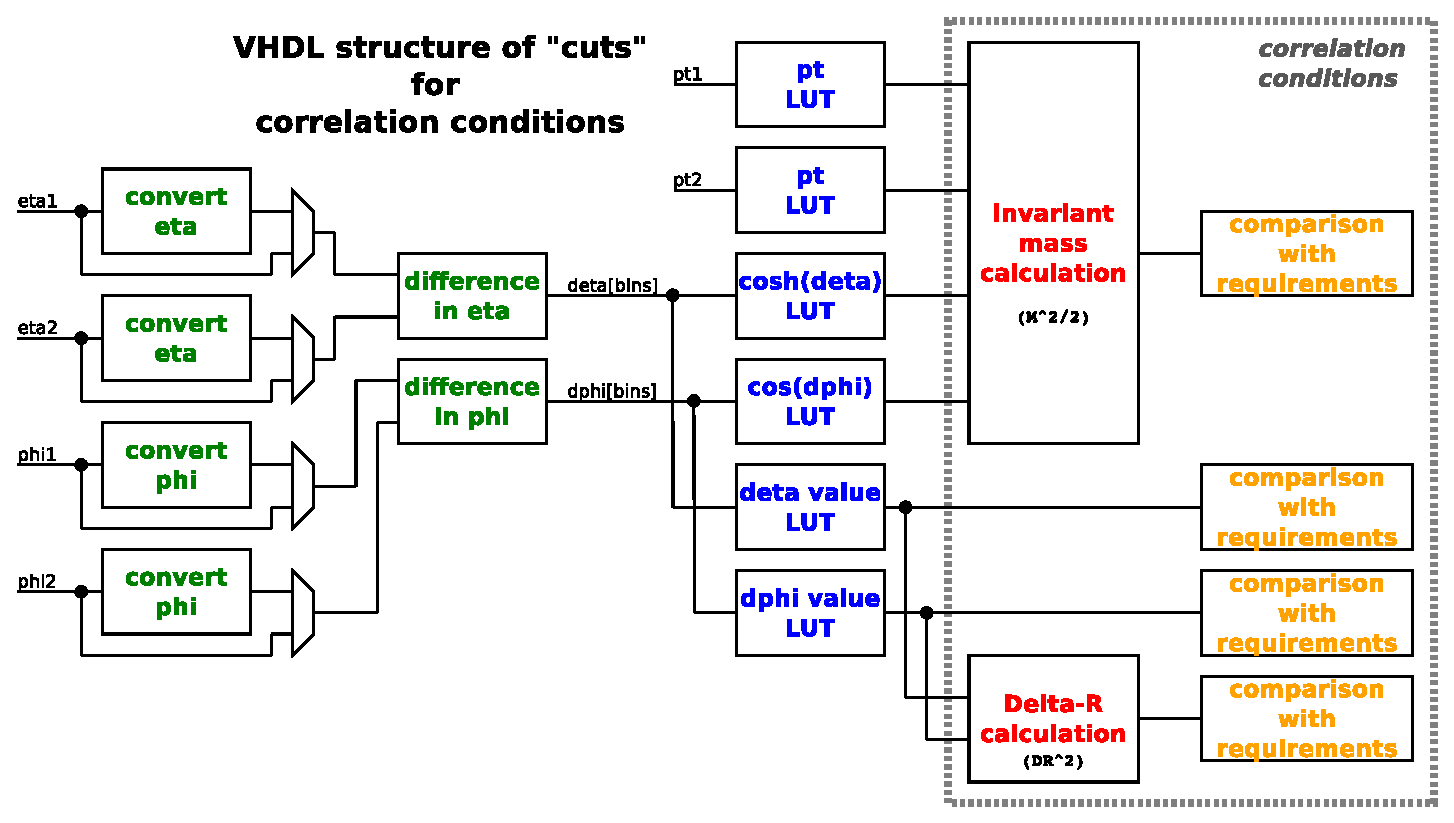
\includegraphics[width=15cm]{figures/scheme_vhdl_cuts_correllation_condition}
\caption{VHDL structure of cuts for correlation conditions} 
\label{fig:gtl:scheme_vhdl_cuts_correllation_condition}
\end{figure}

\paragraph{Calculation of cuts}
\label{sec:gtl:delta_r_calculation}

Calculation of $\Delta\eta$ and $\Delta\varphi$ see section "Calculation of differences in $\eta$ and $\varphi$" (\ref{sec:gtl:calculation_differences}).

\subparagraph{$\Delta$$R$ calculation}
\label{sec:gtl:delta_r_calculation}

The calculation of $\Delta$$R$ of two objects is done with formula:\\ $\Delta$$R=\sqrt{(\eta_1-\eta_2)^2+(\varphi_1-\varphi_2)^2}$.\\
In the TME there are two thresholds for $\Delta$$R$: "greater/equal lower limit" and "less/equal upper limit", given in floating point notation
with one position after decimal point.
The comparison in VHDL is done with $\Delta$$R^2$ (no square root in VHDL), thresholds for $\Delta$$R^2$ are provided by VHDL-Producer.

\subparagraph{Invariant mass calculation}
\label{sec:gtl:inv_mass_calculation}

The calculation of Invariant mass of two objects is done with formula:\\
% M=$\sqrt{2 \times pt_1 \times pt_2 \times (\cosh(\eta_1-\eta_2)-\cos(\varphi_1-\varphi_2))}$.\\
M=$\sqrt{2 pt_1  pt_2 (\cosh(\eta_1-\eta_2)-\cos(\varphi_1-\varphi_2))}$.\\
In the TME there are two thresholds for M: "greater/equal lower limit" and "less/equal upper limit", given in GeV (floating point notation)
with one position after decimal point in even numbers.\footnote{even numbers to get a precision of one position after decimal point after dividion by 2,
because VHDL-Producer calculates thresholds for $\frac{M^2}{2}$, which includes a division by 2.}
The comparison in VHDL is done with $\frac{M^2}{2}$ (no square root in VHDL), thresholds for $\frac{M^2}{2}$ are provided by VHDL-Producer.

\subparagraph{Transverse mass calculation}
\label{sec:gtl:transverse_mass_calculation}

The calculation of Transverse mass of two objects is done with formula:\\
% M=$\sqrt{2 \times pt_1 \times pt_2 \times (1-\cos(\varphi_1-\varphi_2))}$.\\
M=$\sqrt{2 pt_1 pt_2 (1-\cos(\varphi_1-\varphi_2))}$.\\
In the TME there are two thresholds for M: "greater/equal lower limit" and "less/equal upper limit", given in GeV (floating point notation)
with one position after decimal point in even numbers.
The comparison in VHDL is done with $\frac{M^2}{2}$ (no square root in VHDL), thresholds for $\frac{M^2}{2}$ are provided by VHDL-Producer.

\subparagraph{Two-body pt calculation}
\label{sec:gtl:twobody_pt_calculation}

The calculation of two-body pt is done with formula:\\
% pt=$\sqrt{pt^2_1 + pt^2_2 + 2 \times pt_1 \times pt_2 \times (\cos(\varphi_1) \times \cos(\varphi_2) + \sin(\varphi_1) \times \sin(\varphi_2))}$
pt=$\sqrt{pt^2_1 + pt^2_2 + 2  pt_1 pt_2 (\cos(\varphi_1) \cos(\varphi_2) + \sin(\varphi_1) \sin(\varphi_2))}$

In the TME there is one threshold for pt, given in GeV (floating point notation) with one position after decimal point.
The comparison in VHDL is done with ${pt^2}$ (no square root in VHDL), threshold for ${pt^2}$ is provided by VHDL-Producer.

\paragraph{Correlation condition modules}
\label{sec:gtl:correlation_condition_modules}

As described in section Correlation conditions (\ref{sec:gtl:correlation_conditions}), correlations of two object types are done. Therefore several modules are provided
with possible correlations (objects 1-objects 2):
\begin{itemize}
\item Correlation condition with calorimeter objects\\(\texttt{calo\_calo\_correlation\_condition.vhd}:
\egamma-\egamma, \egamma-jet, \egamma-tau, jet-jet, jet-tau and tau-tau are possible.)
\item Correlation condition with calorimeter objects and muons objects\\(\texttt{calo\_muon\_correlation\_condition.vhd}: \egamma-muon, jet-muon and tau-muon are possible.)
\item Correlation condition with muon objects\\(\texttt{muon\_muon\_correlation\_condition.vhd})
\item Correlation condition with calorimeter objects and \esums (\etm, ET$_{miss}^{HF}$ and \htm only)\\(\texttt{calo\_esums\_correlation\_condition.vhd}: \egamma-etm, jet-etm, tau-etm,
\egamma-htm, jet-htm, tau-htm, \egamma-etmhf, jet-etmhf and tau-etmhf are possible.)
\item Correlation condition with muon objects and \esums (\etm, ET$_{miss}^{HF}$ and \htm only)\\(\texttt{muon\_esums\_correlation\_condition.vhd}: muon-etm, muon-etmhf and muon-htm are possible.)
\end{itemize}

\subparagraph{Calo Calo Correlation condition module}
\label{sec:gtl:calo_calo_correlation_condition_module}

The calo calo correlation condition module contains two "Single object requirement conditions" for different types of calo objects (\egamma, jet or tau) or same type with data from different
bunch-crossings as one possible mode and a "Double objects requirement condition" for calo objects of same type and same bunch-crossing as a second mode (selection is done by a parameter in the
generic list of \texttt{calo\_calo\_correlation\_condition.vhd} named "same\_bx").\\
In addition there are "Cuts" for differences in $\eta$ (DETA) and $\varphi$ (DPHI) or a calculation of $\Delta$$R$ (DR) or a calculation of mass (MASS), see Figure~\ref{fig:gtl:scheme_vhdl_cuts_correllation_condition}.\\
The cut of mass is available for Invariant mass or Transverse mass or one of both with two-body pt.\\
The differences in $\eta$ and $\varphi$ are calculated in bins. These differences in bins are converted to numbers (by LUTs, e.g. \small{EG\_EG\_DIFF\_ETA\_LUT, EG\_EG\_DIFF\_PHI\_LUT}\normalsize, ...),
which represents values of differences (multiples of units in $\eta$ and $\varphi$).
These values given in the LUTs are calculated as floating-point values (based on the scales of $\eta$ and $\varphi$), which are multiplied by a factor and truncated to an integer value.
So, in the LUTs we have integer values, the factor is 10\textsuperscript{\tiny{precision}\normalsize}. This "precision" is a parameter given for certain LUTs.\\

\textbf{Remark:} Definitions of scales (see Tables \ref{tab:gtl:calo_eta_scale}, \ref{tab:gtl:calo_phi_scale}, \ref{tab:gtl:muon_eta_scale} and \ref{tab:gtl:muon_phi_scale}):
\begin{itemize}
\item Calorimeter objects:
\item $\eta$ bin width = $\frac{0.087}{2}$ (bin 0 from 0.0 to $\frac{0.087}{2}$)
\item $\phi$ bin width = $\frac{2\pi}{144}$ (bin 0 from 0.0 to $\frac{2\pi}{144}$)
\end{itemize}

The contents of the LUTs for $\cosh(\Delta\eta)$ (\small{EG\_EG\_COSH\_DETA\_LUT}\normalsize, ...) and $\cos(\Delta\varphi)$ (\small{EG\_EG\_COS\_DPHI\_LUT}\normalsize, ...) for Invariant mass
(formular see \ref{sec:gtl:inv_mass_calculation}) and Transverse mass (formular see \ref{sec:gtl:transverse_mass_calculation}) are created by calculating hyperbolic cosine and cosine, rounding-up at the 3\textsuperscript{rd} position after decimal point,
and multiplying by 1000 to get integer values.\footnote{Definition of "\texttt{constant \small{CALO\_INV\_MASS\_COSH\_COS\_PRECISION}\normalsize ..."} in file \texttt{gtl\_pkg.vhd}.
1000 from 10\textsuperscript{\tiny{CALO\_INV\_MASS\_COSH\_COS\_PRECISION}}\normalsize.}\\
The contents of the LUTs for $\cos(\varphi)$ (\small{CALO\_COS\_PHI\_LUT}\normalsize) and $\sin(\varphi)$ (\small{CALO\_SIN\_PHI\_LUT}\normalsize) for two-body pt
(formular see \ref{sec:gtl:twobody_pt_calculation}) are created by calculating cosine and sine, rounding-up at the 3\textsuperscript{rd} position after decimal point and 
multiplying by 1000 to get integer values.\\
The condition is complied, if at least one comparison between object parameters and requirements is valid for the both "Single object requirement condition" or the "Double objects requirement condition"
and the results of selected "Cuts" are inside of a range (upper and lower limit).
This limits are parts of the "generic" list of the entity declaration of the module and are expressed in hex notation. The limits for DETA and DPHI
are expressed with a precision of 3\textsuperscript{rd} position after decimal point, for DR and MASS with 1\textsuperscript{st} position after decimal point.

For the VHDL entity declaration of calo calo correlation condition module (version 4) in \texttt{calo\_calo\_correlation\_condition.vhd}, see Listing~\ref{lst:calo_calo_correlation_condition_vhd}.\\
\clearpage
%% "automatic generation" of listings (see /scripts/extract_entities.sh)
\lstinputlisting[label=lst:calo_calo_correlation_condition_vhd,language=VHDL,caption=Entity declaration of \texttt{calo\_calo\_correlation\_condition.vhd}]{interfaces/calo_calo_correlation_condition.vhd}

\begin{longtable}{>{\footnotesize}l >{\footnotesize}p{.65\columnwidth}}
\caption{Explanation of Listing~\ref{lst:calo_calo_correlation_condition_vhd}}\\
\hline 
{Item} & {Explanation}\\
\hline 
\endhead
\verb|same_bx| & boolean indicating whether data are from same Bx - 'true' for same Bx.\\
\verb|deta_cut| & boolean for using DETA cut.\\
\verb|dphi_cut| & boolean for using DPHI cut.\\
\verb|dr_cut| & boolean for using DR cut.\\
\verb|mass_cut| & boolean for using MASS cut.\\
\verb|mass_type| & selection of mass type (INVARIANT\_MASS\_TYPE, INVARIANT\_MASS\_PT\_TYPE, TRANSVERSE\_MASS\_TYPE or TRANSVERSE\_MASS\_PT\_TYPE are allowed).\\
\verb|calo1_object_low| & low index of object range (valid numbers: 0..11).\\
\verb|calo1_object_high| & high index of object range (valid numbers: 0..11, but greater or equal calo1\_object\_low).\\
\verb|et_ge_mode_calo1| & 'mode-selection' for the \et comparator. Valid strings are 'true' and 'false' (type is boolean), 'true' means comparator works on greater/equal, 'false' means equal (for tests only).\\
\verb|obj_type_calo1| & selection of calo1 object type (EG\_TYPE, JET\_TYPE or TAU\_TYPE are allowed)\\
\verb|et_threshold_calo1| & threshold value for comparison in \et.\\
\verb|nr_eta_windows_calo1| & integer value for number of $\eta$ cuts.\\
\verb|eta_w1_upper_limit_calo1| & "upper limit" of "window"-comparator 1 for $\eta$.\\
\verb|eta_w1_lower_limit_calo1| & "lower limit" of "window"-comparator 1 for $\eta$.\\
\verb|eta_w2_upper_limit_calo1| & "upper limit" of "window"-comparator 2 for $\eta$.\\
\verb|eta_w2_lower_limit_calo1| & "lower limit" of "window"-comparator 2 for $\eta$.\\
\verb|eta_w3_upper_limit_calo1| & "upper limit" of "window"-comparator 3 for $\eta$.\\
\verb|eta_w3_lower_limit_calo1| & "lower limit" of "window"-comparator 3 for $\eta$.\\
\verb|eta_w4_upper_limit_calo1| & "upper limit" of "window"-comparator 4 for $\eta$.\\
\verb|eta_w4_lower_limit_calo1| & "lower limit" of "window"-comparator 4 for $\eta$.\\
\verb|eta_w5_upper_limit_calo1| & "upper limit" of "window"-comparator 5 for $\eta$.\\
\verb|eta_w5_lower_limit_calo1| & "lower limit" of "window"-comparator 5 for $\eta$.\\
\verb|phi_full_range_calo1| & boolean to set full range of $\varphi$.\\
\verb|phi_w1_upper_limit_calo1| & "upper limit" of "window"-comparator 1 for $\varphi$.\\
\verb|phi_w1_lower_limit_calo1| & "lower limit" of "window"-comparator 1 for $\varphi$.\\
\verb|phi_w2_ignore_calo1| & boolean to ignore "window"-comparator 2 for $\varphi$.\\
\verb|phi_w2_upper_limit_calo1| & "upper limit" of "window"-comparator 2 for $\varphi$.\\
\verb|phi_w2_lower_limit_calo1| & "lower limit" of "window"-comparator 2 for $\varphi$.\\
\verb|iso_lut_calo1| & content of LUT (4 bits) for isolation comparison.\\
\verb|calo2_object_low| & low index of object range (valid numbers: 0..11).\\
\verb|calo2_object_high| & high index of object range (valid numbers: 0..11, but greater or equal calo2\_object\_low).\\
\verb|et_ge_mode_calo2| & 'mode-selection' for the \et comparator. Valid strings are 'true' and 'false' (type is boolean), 'true' means comparator works on greater/equal, 'false' means equal (for tests only)\\
\verb|obj_type_calo2| & selection of calo2 object type (EG\_TYPE, JET\_TYPE or TAU\_TYPE are allowed)\\
\verb|et_threshold_calo2| & threshold value for comparison in \et.\\
\verb|nr_eta_windows_calo2| & integer value for number of $\eta$ cuts.\\
\verb|eta_w1_upper_limit_calo2| & "upper limit" of "window"-comparator 1 for $\eta$.\\
\verb|eta_w1_lower_limit_calo2| & "lower limit" of "window"-comparator 1 for $\eta$.\\
\verb|eta_w2_upper_limit_calo2| & "upper limit" of "window"-comparator 2 for $\eta$.\\
\verb|eta_w2_lower_limit_calo2| & "lower limit" of "window"-comparator 2 for $\eta$.\\
\verb|eta_w3_upper_limit_calo2| & "upper limit" of "window"-comparator 3 for $\eta$.\\
\verb|eta_w3_lower_limit_calo2| & "lower limit" of "window"-comparator 3 for $\eta$.\\
\verb|eta_w4_upper_limit_calo2| & "upper limit" of "window"-comparator 4 for $\eta$.\\
\verb|eta_w4_lower_limit_calo2| & "lower limit" of "window"-comparator 4 for $\eta$.\\
\verb|eta_w5_upper_limit_calo2| & "upper limit" of "window"-comparator 5 for $\eta$.\\
\verb|eta_w5_lower_limit_calo2| & "lower limit" of "window"-comparator 5 for $\eta$.\\
\verb|phi_full_range_calo2| & boolean to set full range of $\varphi$.\\
\verb|phi_w1_upper_limit_calo2| & "upper limit" of "window"-comparator 1 for $\varphi$.\\
\verb|phi_w1_lower_limit_calo2| & "lower limit" of "window"-comparator 1 for $\varphi$.\\
\verb|phi_w2_ignore_calo2| & boolean to ignore "window"-comparator 2 for $\varphi$.\\
\verb|phi_w2_upper_limit_calo2| & "upper limit" of "window"-comparator 2 for $\varphi$.\\
\verb|phi_w2_lower_limit_calo2| & "lower limits" of "window"-comparator 2 for $\varphi$.\\
\verb|iso_lut_calo2| & content of LUT (4 bits) for isolation comparison.\\
\verb|diff_eta_upper_limit| & "upper limit" of "window"-comparator for comparison of differences in $\eta$ (hex value).\\
\verb|diff_eta_lower_limit| & "lower limit" of "window"-comparator for comparison of differences in $\eta$ (hex value).\\
\verb|diff_phi_upper_limit| & "upper limit" of "window"-comparator for comparison of differences in $\varphi$ (hex value).\\
\verb|diff_phi_lower_limit| & "lower limit" of "window"-comparator for comparison of differences in $\varphi$ (hex value).\\
\verb|dr_upper_limit| & "upper limit" of "window"-comparator for comparison of $\Delta$$R^2$ (hex value).\\
\verb|dr_lower_limit| & "lower limit" of "window"-comparator for comparison of $\Delta$$R^2$ (hex value).\\
\verb|DETA_DPHI_VECTOR_WIDTH| & vector width of $\Delta\eta$ and $\Delta\varphi$ for calculation of $\Delta$$R^2$.\\
\verb|DETA_DPHI_PRECISION| & position after decimal point for DETA and DPHI.\\
\verb|mass_upper_limit| & "upper limit" of "window"-comparator for comparison of $\frac{M^2}{2}$ (hex value).\\
\verb|mass_lower_limit| & "lower limit" of "window"-comparator for comparison of $\frac{M^2}{2}$ (hex value).\\
\verb|MASS_PRECISION| & position after decimal point for $\frac{M^2}{2}$.\\
\verb|pt1_width| & number of bits of pt1.\\
\verb|pt2_width| & number of bits of pt2.\\
\verb|MASS_COSH_COS_PRECISION| & position after decimal point for $\cosh(\Delta\eta)$ and $\cos(\Delta\varphi)$.\\
\verb|cosh_cos_width| & number of bits for the maximum value in the LUT for $\cosh(\Delta\eta)$.\\
\verb|pt_sq_threshold| & threshold value for comparison in two-body pt (${pt^2}$).\\
\verb|sin_cos_width| & number of bits for the maximum value in the LUT for $\cos(\varphi)$ and $\sin(\varphi)$.\\
\verb|PT_PRECISION| & position after decimal point for ${pt^2}$.\\
\verb|PT_SQ_SIN_COS_PRECISION| & position after decimal point for $\cos(\varphi)$ and $\sin(\varphi)$.\\
\verb|lhc_clk| & clock input (LHC clock).\\
\verb|calo1_data_i| & calorimeter input data, structure defined with \texttt{obj\_type\_calo1}.\\
\verb|calo2_data_i| & calorimeter input data, structure defined with \texttt{obj\_type\_calo2}.\\
\verb|diff_eta| & differences in $\eta$, calculated in an instance of module \texttt{sub\_eta\_integer\_obj\_vs\_obj.vhd} in top-of-hierarchy module (\texttt{gtl\_module.vhd}), see \ref{sec:gtl:calculation_differences}.\\
\verb|diff_phi| & differences in $\varphi$, calculated in an instance of module \texttt{sub\_phi\_integer\_obj\_vs\_obj.vhd} in top-of-hierarchy module (\texttt{gtl\_module.vhd}).\\
\verb|pt1| & calo1 \et values [from LUT, in $GeV\times$10].\footnote{value 10 from 10\textsuperscript{\tiny{CALO\_INV\_MASS\_PT\_PRECISION}}}\\
\verb|pt2| & calo2 \et values [from LUT, in $GeV\times$10].\\
\verb|cosh_deta| & $\cosh(\Delta\eta)$ values [from LUT, $\cosh(\Delta\eta)\times$1000].\footnote{value 1000 from 10\textsuperscript{\tiny{CALO\_INV\_MASS\_COSH\_COS\_PRECISION}}}\\
\verb|cos_dphi| & $\cos(\Delta\varphi)$ values [from LUT, $\cosh(\Delta\varphi)\times$1000].\\
\verb|cos_phi_1| & $\cos(\varphi)$ values from LUT for calo1.\\
\verb|cos_phi_2| & $\cos(\varphi)$ values from LUT for calo2.\\
\verb|sin_phi_1| & $\sin(\varphi)$ values from LUT for calo1.\\
\verb|sin_phi_2| & $\sin(\varphi)$ values from LUT for calo2.\\
\verb|condition_o| & output of condition (routed to Algorithms logic, see \ref{sec:gtl:algorithms_logic}).\\
\hline 
\label{tab:gtl:explanation_calo_calo_correlation_condition_vhd}
\end{longtable}

% \subparagraph{Calo Calo Correlation condition module - template for VHDL-Producer}
% See in Chapter \ref{sec:gtl:templates_tme} and in Listing~\ref{lst:instance_calo_calo_correlation_condition_vhd} for a VHDL-template for VHDL-Producer of
% instantiating a calorimeter-calorimeter-correlation condition (\texttt{calo\_calo\_correlation\_condition.vhd}).\\

\subparagraph{Calo Muon Correlation condition module}
\label{sec:gtl:calo_muon_correlation_condition_module}

The calo muon correlation condition module contains a "Single object requirement condition" for one type of calo objects (\egamma, jet or tau) and a "Single object requirement condition" for muon objects.
In addition with "Cuts" for differences in $\eta$ (DETA), $\varphi$ (DPHI) or a calculation of $\Delta$$R$ (DR) or a calculation of mass (MASS).\\
The cut of mass is available for Invariant mass or Transverse mass or one of both with two-body pt.\\
The differences in $\eta$ and $\varphi$ are calculated in bins. These differences in bins are converted to numbers (by LUTs, e.g. \small{EG\_MUON\_DIFF\_ETA\_LUT, EG\_MUON\_DIFF\_PHI\_LUT}\normalsize, ...),
which represents values of differences (multiples of units in $\eta$ and $\varphi$).
These values given in the LUTs are calculated as floating-point values (based on the scales of $\eta$ and $\varphi$), which are multiplied by a factor and truncated to an integer value.
So, in the LUTs we have integer values, the factor is 10\textsuperscript{\tiny{precision}\normalsize}. This "precision" is a parameter given for certain LUTs.\\
Because of the different scales of calorimeter and muon objects in $\eta$ and $\varphi$, there are LUTs for conversion the calorimeter bins to muon bins (in \texttt{gtl\_pkg.vhd}:
 e.g. \small{EG\_ETA\_CONV\_2\_MUON\_ETA\_LUT}\normalsize and \small{EG\_PHI\_CONV\_2\_MUON\_PHI\_LUT}\normalsize).\\\\
\textbf{Remark:}\\
The center value of bins are used as reference value for conversion.
The content of \small{EG\_ETA\_CONV\_2\_MUON\_ETA\_LUT}\normalsize is calculated with formular:\\ "converted-calo-eta[bin] = calo-eta[bin] $\times$ 4 + 2",\\
of \small{EG\_PHI\_CONV\_2\_MUON\_PHI\_LUT}\normalsize with formular:\\
"converted-calo-phi[bin] = calo-phi[bin] $\times$ 4 + 2".\\
The conversion calculations are preliminary, others may be proposed.\\\\
Definitions of scales (see Tables \ref{tab:gtl:calo_eta_scale}, \ref{tab:gtl:calo_phi_scale}, \ref{tab:gtl:muon_eta_scale} and \ref{tab:gtl:muon_phi_scale}):
\begin{itemize}
\item Calorimeter objects:
\begin{itemize}
\item $\eta$ bin width = $\frac{0.087}{2}$ (bin 0 from 0.0 to $\frac{0.087}{2}$)
\item $\phi$ bin width = $\frac{2\pi}{144}$ (bin 0 from 0.0 to $\frac{2\pi}{144}$)
\end{itemize}
\item Muon objects:
\begin{itemize}
\item $\eta$ bin width = $\frac{0.087}{8}$ (bin 0 from \small{0.5}$\times\frac{-0.087}{8}$ to \small{0.5}$\times\frac{+0.087}{8}$)
\item $\phi$ bin width = $\frac{2\pi}{576}$ (bin 0 from 0.0 to $\frac{2\pi}{576}$)
\end{itemize}
\end{itemize}

\begin{figure}[htb]
\centering
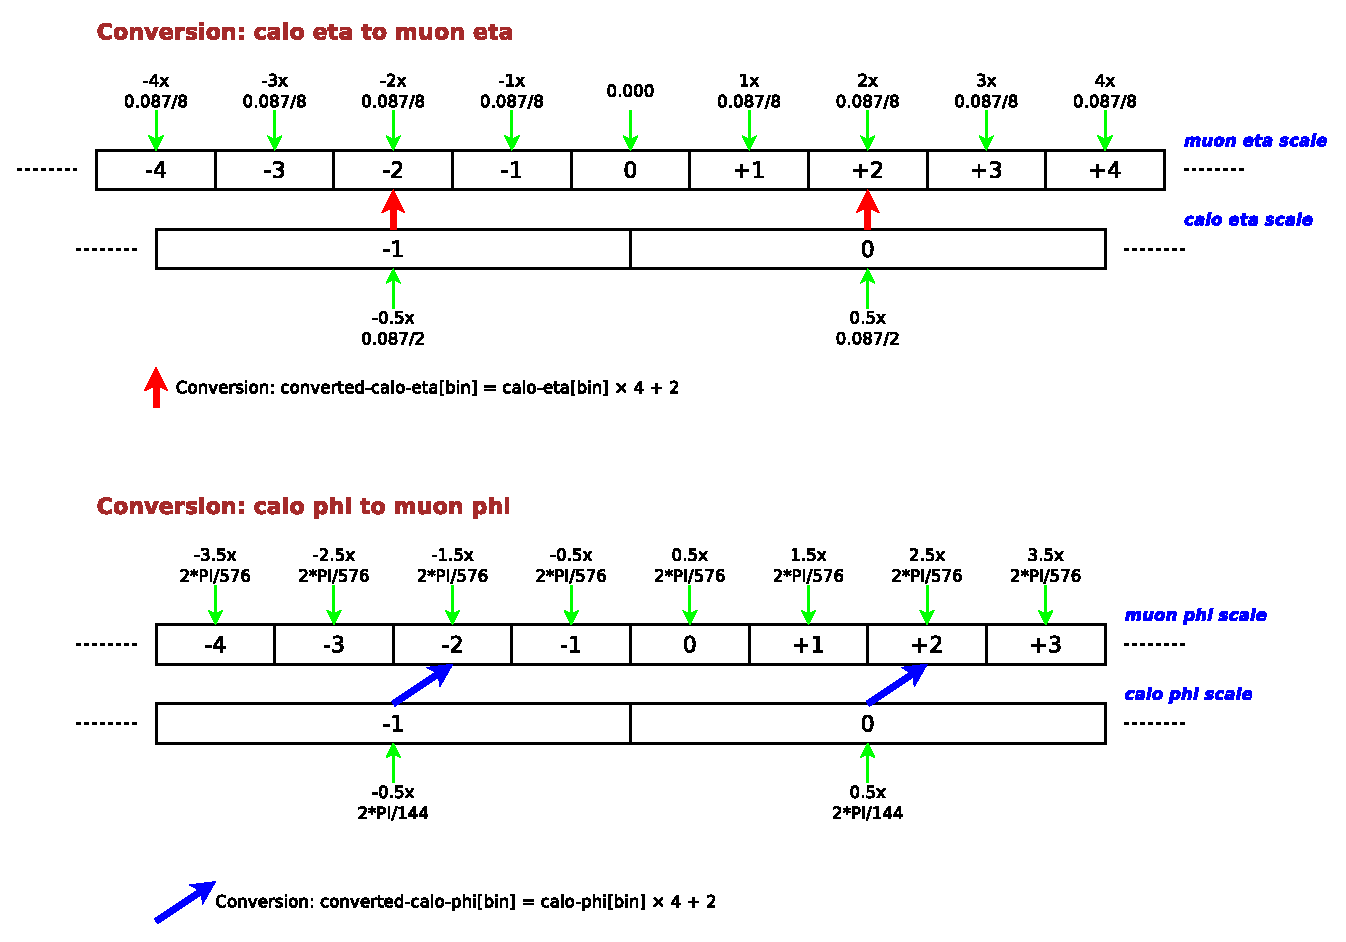
\includegraphics[width=15cm]{figures/convert_scheme_calo_2_muon_eta_phi}
\caption{Conversion of calorimeter $\eta$ and $\varphi$ to muon scales} 
\label{fig:gtl:convert_scheme_calo_2_muon_eta_phi}
\end{figure}

The contents of the LUTs for $\cosh(\Delta\eta)$ (\small{EG\_MUON\_COSH\_DETA\_LUT}\normalsize, ...) and $\cos(\Delta\varphi)$ (\small{EG\_MUON\_COS\_DPHI\_LUT}\normalsize, ...) for Invariant mass
(formular see \ref{sec:gtl:inv_mass_calculation}) and Transverse mass (formular see \ref{sec:gtl:transverse_mass_calculation}) are created by calculating hyperbolic cosine and cosine, 
rounding-up at the 4\textsuperscript{th} position after decimal point, and multiplying by 10000
(10\textsuperscript{\tiny{CALO\_MUON\_INV\_MASS\_COSH\_COS\_PRECISION}}\normalsize) to get integer values.\footnote{Definition of "\texttt{constant \small{CALO\_MUON\_INV\_MASS\_COSH\_COS\_PRECISION}\normalsize} ...",
"\texttt{constant \small{EG\_ETA\_CONV\_2\_MUON\_ETA\_LUT}\normalsize} ..." and "\texttt{constant \small{EG\_PHI\_CONV\_2\_MUON\_PHI\_LUT}\normalsize} ..." in file \texttt{gtl\_pkg.vhd}.}\\
The contents of the LUTs for $\cos(\varphi)$ (\small{CALO\_COS\_PHI\_LUT and MUON\_COS\_PHI\_LUT}\normalsize) and $\sin(\varphi)$ (\small{CALO\_SIN\_PHI\_LUT and MUON\_SIN\_PHI\_LUT}\normalsize) for two-body pt 
(formular see \ref{sec:gtl:twobody_pt_calculation}) are created by calculating cosine and sine, rounding-up at the 3\textsuperscript{rd} position after decimal point,
and multiplying by 1000 to get integer values.\\
The condition is complied, if at least one comparison between object parameters and requirements is valid for the both "Single object requirement condition" and the results of selected "Cuts" are inside of
a range (upper and lower limit). This limits are parts of the "generic" list of the entity declaration of the module and are expressed in hex notation. The limits for DETA and DPHI
are expressed with the 3\textsuperscript{rd} position after decimal point, for DR and MASS with the 1\textsuperscript{st} position after decimal point.

For the VHDL entity declaration of calo muon correlation condition module (version 3) in \texttt{calo\_muon\_correlation\_condition.vhd}, see Listing~\ref{lst:calo_muon_correlation_condition_vhd}.\\
\clearpage
%% "automatic generation" of listings (see /scripts/extract_entities.sh)
\lstinputlisting[label=lst:calo_muon_correlation_condition_vhd,language=VHDL,caption=Entity declaration of \texttt{calo\_muon\_correlation\_condition.vhd}]{interfaces/calo_muon_correlation_condition.vhd}

\begin{longtable}{>{\footnotesize}l >{\footnotesize}p{.65\columnwidth}}
\caption{Explanation of Listing~\ref{lst:calo_muon_correlation_condition_vhd}}\\
\hline 
{Item} & {Explanation}\\
\hline 
\endhead
\verb|deta_cut| & boolean for using DETA cut.\\
\verb|dphi_cut| & boolean for using DPHI cut.\\
\verb|dr_cut| & boolean for using DR cut.\\
\verb|mass_cut| & boolean for using MASS cut.\\
\verb|mass_type| & selection of mass type (INVARIANT\_MASS\_TYPE, INVARIANT\_MASS\_PT\_TYPE, TRANSVERSE\_MASS\_TYPE or TRANSVERSE\_MASS\_PT\_TYPE are allowed).\\
\verb|calo_object_low| & low index of object range (valid numbers: 0..11).\\
\verb|calo_object_high| & high index of object range (valid numbers: 0..11, but greater or equal calo\_object\_low).\\
\verb|calo_et_ge_mode_calo| & 'mode-selection' for the \et comparator. Valid strings are 'true' and 'false' (type is boolean), 'true' means comparator works on greater/equal, 'false' means equal (for tests only).\\
\verb|obj_type_calo| & selection of calo object type (EG\_TYPE, JET\_TYPE or TAU\_TYPE are allowed)\\
\verb|et_threshold_calo| & threshold value for comparison in \et.\\
\verb|nr_eta_windows_calo| & integer value for number of $\eta$ cuts.\\
\verb|eta_w1_upper_limit_calo| & "upper limit" of "window"-comparator 1 for $\eta$.\\
\verb|eta_w1_lower_limit_calo| & "lower limit" of "window"-comparator 1 for $\eta$.\\
\verb|eta_w2_upper_limit_calo| & "upper limit" of "window"-comparator 2 for $\eta$.\\
\verb|eta_w2_lower_limit_calo| & "lower limit" of "window"-comparator 2 for $\eta$.\\
\verb|eta_w3_upper_limit_calo| & "upper limit" of "window"-comparator 3 for $\eta$.\\
\verb|eta_w3_lower_limit_calo| & "lower limit" of "window"-comparator 3 for $\eta$.\\
\verb|eta_w4_upper_limit_calo| & "upper limit" of "window"-comparator 4 for $\eta$.\\
\verb|eta_w4_lower_limit_calo| & "lower limit" of "window"-comparator 4 for $\eta$.\\
\verb|eta_w5_upper_limit_calo| & "upper limit" of "window"-comparator 5 for $\eta$.\\
\verb|eta_w5_lower_limit_calo| & "lower limit" of "window"-comparator 5 for $\eta$.\\
\verb|phi_full_range_calo| & boolean to set full range of $\varphi$.\\
\verb|phi_w1_upper_limit_calo| & "upper limit" of "window"-comparator 1 for $\varphi$.\\
\verb|phi_w1_lower_limit_calo| & "lower limit" of "window"-comparator 1 for $\varphi$.\\
\verb|phi_w2_ignore_calo| & boolean to ignore "window"-comparator 2 for $\varphi$.\\
\verb|phi_w2_upper_limit_calo| & "upper limit" of "window"-comparator 2 for $\varphi$.\\
\verb|phi_w2_lower_limit_calo| & "lower limit" of "window"-comparator 2 for $\varphi$.\\
\verb|iso_lut_calo| & content of LUT (4 bits) for isolation comparison.\\
\verb|muon_object_low| & low index of object range (valid numbers: 0..7).\\
\verb|muon_object_high| & high index of object range (valid numbers: 0..7, but greater or equal muon\_object\_low).\\
\verb|pt_ge_mode_muon| & 'mode-selection' for the \pt comparator. Valid strings are 'true' and 'false' (type is boolean), 'true' means comparator works on greater/equal, 'false' means equal (for tests only)\\
\verb|pt_threshold_muon| & threshold value for comparison in \pt.\\
\verb|nr_eta_windows_muon| & integer value for number of $\eta$ cuts.\\
\verb|eta_w1_upper_limit_muon| & "upper limit" of "window"-comparator 1 for $\eta$.\\
\verb|eta_w1_lower_limit_muon| & "lower limit" of "window"-comparator 1 for $\eta$.\\
\verb|eta_w2_upper_limit_muon| & "upper limit" of "window"-comparator 2 for $\eta$.\\
\verb|eta_w2_lower_limit_muon| & "lower limit" of "window"-comparator 2 for $\eta$.\\
\verb|eta_w3_upper_limit_muon| & "upper limit" of "window"-comparator 3 for $\eta$.\\
\verb|eta_w3_lower_limit_muon| & "lower limit" of "window"-comparator 3 for $\eta$.\\
\verb|eta_w4_upper_limit_muon| & "upper limit" of "window"-comparator 4 for $\eta$.\\
\verb|eta_w4_lower_limit_muon| & "lower limit" of "window"-comparator 4 for $\eta$.\\
\verb|eta_w5_upper_limit_muon| & "upper limit" of "window"-comparator 5 for $\eta$.\\
\verb|eta_w5_lower_limit_muon| & "lower limit" of "window"-comparator 5 for $\eta$.\\
\verb|phi_full_range_muon| & boolean to set full range of $\varphi$.\\
\verb|phi_w1_upper_limit_muon| & "upper limit" of "window"-comparator 1 for $\varphi$.\\
\verb|phi_w1_lower_limit_muon| & "lower limit" of "window"-comparator 1 for $\varphi$.\\
\verb|phi_w2_ignore_muon| & boolean to ignore "window"-comparator 2 for $\varphi$.\\
\verb|phi_w2_upper_limit_muon| & "upper limit" of "window"-comparator 2 for $\varphi$.\\
\verb|phi_w2_lower_limit_muon| & "lower limits" of "window"-comparator 2 for $\varphi$.\\
\verb|requested_charge_muon| & string for requested charge ("pos" means "positive charge", "neg" means "negative charge" and "ign" means "ignore charge").\\
\verb|qual_lut_muon| & content of LUT (16 bits) for quality comparison.\\
\verb|iso_lut_muon| & content of LUT (4 bits) for isolation comparison.\\
\verb|upt_cut_muon| & boolean for using unconstraint \pt cuts.\\
\verb|upt_upper_limit_muon| & "upper limit" of unconstraint \pt.\\
\verb|upt_lower_limit_muon| & "lower limit" of unconstraint \pt.\\
\verb|ip_lut_muon| & content of LUTs (4 bits) for impact parameter.\\
\verb|diff_eta_upper_limit| & "upper limit" of "window"-comparator for comparison of differences in $\eta$ (hex value).\\
\verb|diff_eta_lower_limit| & "lower limit" of "window"-comparator for comparison of differences in $\eta$ (hex value).\\
\verb|diff_phi_upper_limit| & "upper limit" of "window"-comparator for comparison of differences in $\varphi$ (hex value).\\
\verb|diff_phi_lower_limit| & "lower limit" of "window"-comparator for comparison of differences in $\varphi$ (hex value).\\
\verb|dr_upper_limit| & "upper limit" of "window"-comparator for comparison of $\Delta$$R^2$ (hex value).\\
\verb|dr_lower_limit| & "lower limit" of "window"-comparator for comparison of $\Delta$$R^2$ (hex value).\\
\verb|DETA_DPHI_VECTOR_WIDTH| & vector width of $\Delta\eta$ and $\Delta\varphi$ for calculation of $\Delta$$R^2$.\\
\verb|DETA_DPHI_PRECISION| & position after decimal point for DETA and DPHI.\\
\verb|mass_upper_limit| & "upper limit" of "window"-comparator for comparison of $\frac{M^2}{2}$ (hex value).\\
\verb|mass_lower_limit| & "lower limit" of "window"-comparator for comparison of $\frac{M^2}{2}$ (hex value).\\
\verb|MASS_PRECISION| & position after decimal point for $\frac{M^2}{2}$.\\
\verb|pt1_width| & number of bits of pt1.\\
\verb|pt2_width| & number of bits of pt2.\\
\verb|MASS_COSH_COS_PRECISION| & position after decimal point for $\cosh(\Delta\eta)$ and $\cos(\Delta\varphi)$.\\
\verb|cosh_cos_width| & number of bits for the maximum value in the LUT for $\cosh(\Delta\eta)$.\\
\verb|pt_sq_threshold| & threshold value for comparison in two-body pt (${pt^2}$).\\
\verb|sin_cos_width_1| & number of bits for the maximum value in the LUT for $\cos(\varphi)$ and $\sin(\varphi)$ of calos.\\
\verb|sin_cos_width_2| & number of bits for the maximum value in the LUT for $\cos(\varphi)$ and $\sin(\varphi)$ of muon.\\
\verb|PT_PRECISION| & position after decimal point for ${pt^2}$.\\
\verb|PT_SQ_SIN_COS_PRECISION| & position after decimal point for $\cos(\varphi)$ and $\sin(\varphi)$.\\
\verb|lhc_clk| & clock input (LHC clock).\\
\verb|calo_data_i| & calorimeter input data, structure defined with \texttt{obj\_type\_calo}.\\
\verb|muon_data_i| & muon input data.\\
\verb|diff_eta| & differences in $\eta$, calculated in an instance of module \texttt{sub\_eta\_integer\_obj\_vs\_obj.vhd} in top-of-hierarchy module (\texttt{gtl\_module.vhd}), see \ref{sec:gtl:calculation_differences}.\\
\verb|diff_phi| & differences in $\varphi$, calculated in an instance of module \texttt{sub\_phi\_integer\_obj\_vs\_obj.vhd} in top-of-hierarchy module (\texttt{gtl\_module.vhd}).\\
\verb|pt1| & calo \et values [from LUT, in $GeV\times$10].\footnote{value 10 from 10\textsuperscript{\tiny{CALO\_MUON\_INV\_MASS\_PT\_PRECISION}}}\\
\verb|pt2| & muon \pt values [from LUT, in $GeV \times$10].\\
\verb|cosh_deta| & $\cosh(\Delta\eta)$ values [from LUT, $\cosh(\Delta\eta)\times$10000].\footnote{value 10000 from 10\textsuperscript{\tiny{CALO\_MUON\_INV\_MASS\_COSH\_COS\_PRECISION}}}\\
\verb|cos_dphi| & $\cos(\Delta\varphi)$ values [from LUT, $\cosh(\Delta\varphi)\times$10000].\\
\verb|cos_phi_1| & $\cos(\varphi)$ values from LUT for calo.\\
\verb|cos_phi_2| & $\cos(\varphi)$ values from LUT for muon.\\
\verb|sin_phi_1| & $\sin(\varphi)$ values from LUT for calo.\\
\verb|sin_phi_2| & $\sin(\varphi)$ values from LUT for muon.\\
\verb|condition_o| & output of condition (routed to Algorithms logic, see \ref{sec:gtl:algorithms_logic}).\\
\hline 
\label{tab:gtl:explanation_calo_muon_correlation_condition_vhd}
\end{longtable}

% \subparagraph{Calo Muon Correlation condition module - template for VHDL-Producer}
% See in Chapter \ref{sec:gtl:templates_tme} and in Listing~\ref{lst:instance_calo_muon_correlation_condition_vhd} for a VHDL-template for VHDL-Producer of
% instantiating a calorimeter-muon-correlation condition (\texttt{calo\_muon\_correlation\_condition.vhd}).\\

\subparagraph{Muon Muon Correlation condition module}
\label{sec:gtl:muon_muon_correlation_condition_module}

The muon muon correlation condition module contains two "Single object requirement conditions" for data from different bunch-crossings as one possible mode
and a "Double objects requirement condition" for muon objects at same bunch-crossing as a second mode (selection is done by a parameter in the
generic list of \texttt{muon\_muon\_correlation\_condition.vhd} named "same\_bx"). In the case of a "Double objects requirement condition", requirements for "requested charge correlations"
are used and a muon charge correlation module (see \ref{sec:gtl:muon_charge_correlation_module}) is required.\\
In addition there are "Cuts" for differences in $\eta$ (DETA), $\varphi$ (DPHI) or a calculation of $\Delta$$R$ (DR) or a calculation of mass (MASS).\\
The cut of mass is available for Invariant mass or Transverse mass or one of both with two-body pt.\\
The differences in $\eta$ and $\varphi$ are calculated in bins. These differences in bins are converted to numbers (by LUTs, e.g. \small{MUON\_MUON\_DIFF\_ETA\_LUT, MUON\_MUON\_DIFF\_PHI\_LUT}\normalsize),
which represents values of differences (multiples of units in $\eta$ and $\varphi$).
These values given in the LUTs are calculated as floating-point values (based on the scales of $\eta$ and $\varphi$), which are multiplied by a factor and truncated to an integer value.
So, in the LUTs we have integer values, the factor is 10\textsuperscript{\tiny{precision}\normalsize}. This "precision" is a parameter given for certain LUTs.\\

\textbf{Remark:} Definitions of scales (see Tables \ref{tab:gtl:muon_eta_scale} and \ref{tab:gtl:muon_phi_scale}):
\begin{itemize}
\item Muon objects:
\item $\eta$ bin width = $\frac{0.087}{8}$ (bin 0 from \small{0.5}$\times\frac{-0.087}{8}$ to \small{0.5}$\times\frac{+0.087}{8}$)
\item $\phi$ bin width = $\frac{2\pi}{576}$ (bin 0 from 0.0 to $\frac{2\pi}{576}$)
\end{itemize}

The contents of the LUTs for $\cosh(\Delta\eta)$ (\small{MUON\_MUON\_COSH\_DETA\_LUT}\normalsize) and $\cos(\Delta\varphi)$ (\small{MUON\_MUON\_COS\_DPHI\_LUT}\normalsize) for Invariant mass
(formular see \ref{sec:gtl:inv_mass_calculation}) and Transverse mass (formular see \ref{sec:gtl:transverse_mass_calculation}) are created by calculating hyperbolic cosine and cosine, 
rounding-up at the 4\textsuperscript{th} position after decimal point,
and multiplying by 10000 to get integer values.\footnote{Definition of "\texttt{constant \small{MUON\_INV\_MASS\_COSH\_COS\_PRECISION}\normalsize"} in file \texttt{gtl\_pkg.vhd}.
10000 from 10\textsuperscript{\tiny{MUON\_INV\_MASS\_COSH\_COS\_PRECISION}}\normalsize.}\\
The contents of the LUTs for $\cos(\varphi)$ (\small{MUON\_COS\_PHI\_LUT}\normalsize) and $\sin(\varphi)$ (\small{MUON\_SIN\_PHI\_LUT}\normalsize) for two-body pt 
(formular see \ref{sec:gtl:twobody_pt_calculation}) are created by calculating cosine and sine, rounding-up at the 3\textsuperscript{rd} position after decimal point,
and multiplying by 1000 to get integer values.\\
The condition is complied, if at least one comparison between object parameters and requirements is valid for the both "Single object requirement condition" or the "Double objects requirement condition"
and the results of selected "Cuts" are inside of a range (upper and lower limit).
This limits are parts of the "generic" list of the entity declaration of the module and are expressed in hex notation. The limits for DETA and DPHI
are expressed with a precision of 3\textsuperscript{rd} position after decimal point, for DR and MASS with 1\textsuperscript{st} position after decimal point.

For the VHDL entity declaration of muon muon correlation condition module in \texttt{muon\_muon\_correlation\_condition.vhd}, see Listing~\ref{lst:muon_muon_correlation_condition_vhd}.\\
\clearpage
%% "automatic generation" of listings (see /scripts/extract_entities.sh)
\lstinputlisting[label=lst:muon_muon_correlation_condition_vhd,language=VHDL,caption=Entity declaration of \texttt{muon\_muon\_correlation\_condition.vhd}]{interfaces/muon_muon_correlation_condition.vhd}

\begin{longtable}{>{\footnotesize}l >{\footnotesize}p{.65\columnwidth}}
\caption{Explanation of Listing~\ref{lst:muon_muon_correlation_condition_vhd}}\\
\hline 
{Item} & {Explanation}\\
\hline 
\endhead
\verb|same_bx| & boolean indicating whether data are from same Bx - 'true' for same Bx.\\
\verb|deta_cut| & boolean for using DETA cut.\\
\verb|dphi_cut| & boolean for using DPHI cut.\\
\verb|dr_cut| & boolean for using DR cut.\\
\verb|mass_cut| & boolean for using MASS cut.\\
\verb|mass_type| & selection of mass type (INVARIANT\_MASS\_TYPE, INVARIANT\_MASS\_PT\_TYPE, TRANSVERSE\_MASS\_TYPE or TRANSVERSE\_MASS\_PT\_TYPE are allowed).\\
\verb|muon_object_low| & low index of object range (valid numbers: 0..7).\\
\verb|muon_object_high| & high index of object range (valid numbers: 0..7, but greater or equal muon\_object\_low).\\
\verb|pt_ge_mode_muon1| & 'mode-selection' for the \pt comparator. Valid strings are 'true' and 'false' (type is boolean), 'true' means comparator works on greater/equal, 'false' means equal (for tests only)\\
\verb|pt_threshold_muon1| & threshold value for comparison in \pt.\\
\verb|nr_eta_windows_muon1| & integer value for number of $\eta$ cuts.\\
\verb|eta_w1_upper_limit_muon1| & "upper limit" of "window"-comparator 1 for $\eta$.\\
\verb|eta_w1_lower_limit_muon1| & "lower limit" of "window"-comparator 1 for $\eta$.\\
\verb|eta_w2_upper_limit_muon1| & "upper limit" of "window"-comparator 2 for $\eta$.\\
\verb|eta_w2_lower_limit_muon1| & "lower limit" of "window"-comparator 2 for $\eta$.\\
\verb|eta_w3_upper_limit_muon1| & "upper limit" of "window"-comparator 3 for $\eta$.\\
\verb|eta_w3_lower_limit_muon1| & "lower limit" of "window"-comparator 3 for $\eta$.\\
\verb|eta_w4_upper_limit_muon1| & "upper limit" of "window"-comparator 4 for $\eta$.\\
\verb|eta_w4_lower_limit_muon1| & "lower limit" of "window"-comparator 4 for $\eta$.\\
\verb|eta_w5_upper_limit_muon1| & "upper limit" of "window"-comparator 5 for $\eta$.\\
\verb|eta_w5_lower_limit_muon1| & "lower limit" of "window"-comparator 5 for $\eta$.\\
\verb|phi_full_range_muon1| & boolean to set full range of $\varphi$.\\
\verb|phi_w1_upper_limit_muon1| & "upper limit" of "window"-comparator 1 for $\varphi$.\\
\verb|phi_w1_lower_limit_muon1| & "lower limit" of "window"-comparator 1 for $\varphi$.\\
\verb|phi_w2_ignore_muon1| & boolean to ignore "window"-comparator 2 for $\varphi$.\\
\verb|phi_w2_upper_limit_muon1| & "upper limit" of "window"-comparator 2 for $\varphi$.\\
\verb|phi_w2_lower_limit_muon1| & "lower limits" of "window"-comparator 2 for $\varphi$.\\
\verb|requested_charge_muon1| & string for requested charge ("pos" means "positive charge", "neg" means "negative charge" and "ign" means "ignore charge").\\
\verb|qual_lut_muon1| & content of LUT (16 bits) for quality comparison.\\
\verb|iso_lut_muon1| & content of LUT (4 bits) for isolation comparison.\\
\verb|upt_cut_muon1| & boolean for using unconstraint \pt cuts.\\
\verb|upt_upper_limit_muon1| & "upper limit" of unconstraint \pt.\\
\verb|upt_lower_limit_muon1| & "lower limit" of unconstraint \pt.\\
\verb|ip_lut_muon1| & content of LUTs (4 bits) for impact parameter.\\
\verb|pt_ge_mode_muon2| & 'mode-selection' for the \pt comparator. Valid strings are 'true' and 'false' (type is boolean), 'true' means comparator works on greater/equal, 'false' means equal (for tests only)\\
\verb|pt_threshold_muon2| & threshold value for comparison in \pt.\\
\verb|nr_eta_windows_muon2| & integer value for number of $\eta$ cuts.\\
\verb|eta_w1_upper_limit_muon2| & "upper limit" of "window"-comparator 1 for $\eta$.\\
\verb|eta_w1_lower_limit_muon2| & "lower limit" of "window"-comparator 1 for $\eta$.\\
\verb|eta_w2_upper_limit_muon2| & "upper limit" of "window"-comparator 2 for $\eta$.\\
\verb|eta_w2_lower_limit_muon2| & "lower limit" of "window"-comparator 2 for $\eta$.\\
\verb|eta_w3_upper_limit_muon2| & "upper limit" of "window"-comparator 3 for $\eta$.\\
\verb|eta_w3_lower_limit_muon2| & "lower limit" of "window"-comparator 3 for $\eta$.\\
\verb|eta_w4_upper_limit_muon2| & "upper limit" of "window"-comparator 4 for $\eta$.\\
\verb|eta_w4_lower_limit_muon2| & "lower limit" of "window"-comparator 4 for $\eta$.\\
\verb|eta_w5_upper_limit_muon2| & "upper limit" of "window"-comparator 5 for $\eta$.\\
\verb|eta_w5_lower_limit_muon2| & "lower limit" of "window"-comparator 5 for $\eta$.\\
\verb|phi_full_range_muon2| & boolean to set full range of $\varphi$.\\
\verb|phi_w1_upper_limit_muon2| & "upper limit" of "window"-comparator 1 for $\varphi$.\\
\verb|phi_w1_lower_limit_muon2| & "lower limit" of "window"-comparator 1 for $\varphi$.\\
\verb|phi_w2_ignore_muon2| & boolean to ignore "window"-comparator 2 for $\varphi$.\\
\verb|phi_w2_upper_limit_muon2| & "upper limit" of "window"-comparator 2 for $\varphi$.\\
\verb|phi_w2_lower_limit_muon2| & "lower limits" of "window"-comparator 2 for $\varphi$.\\
\verb|requested_charge_muon2| & string for requested charge ("pos" means "positive charge", "neg" means "negative charge" and "ign" means "ignore charge").\\
\verb|qual_lut_muon2| & content of LUT (16 bits) for quality comparison.\\
\verb|iso_lut_muon2| & content of LUT (4 bits) for isolation comparison.\\
\verb|upt_cut_muon2| & boolean for using unconstraint \pt cuts.\\
\verb|upt_upper_limit_muon2| & "upper limit" of unconstraint \pt.\\
\verb|upt_lower_limit_muon2| & "lower limit" of unconstraint \pt.\\
\verb|ip_lut_muon2| & content of LUTs (4 bits) for impact parameter.\\
\verb|requested_charge_correlation| & string (2 characters) for requested charge correlation ("ls" means "like sign", "os" means "opposite sign" or "ig" means "ignore").\\
\verb|diff_eta_upper_limit| & "upper limit" of "window"-comparator for comparison of differences in $\eta$ (hex value).\\
\verb|diff_eta_lower_limit| & "lower limit" of "window"-comparator for comparison of differences in $\eta$ (hex value).\\
\verb|diff_phi_upper_limit| & "upper limit" of "window"-comparator for comparison of differences in $\varphi$ (hex value).\\
\verb|diff_phi_lower_limit| & "lower limit" of "window"-comparator for comparison of differences in $\varphi$ (hex value).\\
\verb|dr_upper_limit| & "upper limit" of "window"-comparator for comparison of $\Delta$$R^2$ (hex value).\\
\verb|dr_lower_limit| & "lower limit" of "window"-comparator for comparison of $\Delta$$R^2$ (hex value).\\
\verb|DETA_DPHI_VECTOR_WIDTH| & vector width of $\Delta\eta$ and $\Delta\varphi$ for calculation of $\Delta$$R^2$.\\
\verb|DETA_DPHI_PRECISION| & position after decimal point for DETA and DPHI.\\
\verb|mass_upper_limit| & "upper limit" of "window"-comparator for comparison of $\frac{M^2}{2}$ (hex value).\\
\verb|mass_lower_limit| & "lower limit" of "window"-comparator for comparison of $\frac{M^2}{2}$ (hex value).\\
\verb|MASS_PRECISION| & position after decimal point for $\frac{M^2}{2}$.\\
\verb|pt_width| & number of bits of pt.\\
\verb|MASS_COSH_COS_PRECISION| & position after decimal point for $\cosh(\Delta\eta)$ and $\cos(\Delta\varphi)$.\\
\verb|cosh_cos_width| & number of bits for the maximum value in the LUT for $\cosh(\Delta\eta)$.\\
\verb|pt_sq_threshold| & threshold value for comparison in two-body pt (${pt^2}$).\\
\verb|sin_cos_width| & number of bits for the maximum value in the LUT for $\cos(\varphi)$ and $\sin(\varphi)$.\\
\verb|PT_PRECISION| & position after decimal point for ${pt^2}$.\\
\verb|PT_SQ_SIN_COS_PRECISION| & position after decimal point for $\cos(\varphi)$ and $\sin(\varphi)$.\\
\verb|lhc_clk| & clock input (LHC clock).\\
\verb|muon1_data_i| & muon1 input data.\\
\verb|muon2_data_i| & muon2 input data.\\
\verb|ls_charcorr_double| & array of "like sign" charge correlation for double condition.\\
\verb|os_charcorr_double| & array of "opposite sign" charge correlation for double condition.\\
\verb|diff_eta| & differences in $\eta$, calculated in an instance of module \texttt{sub\_eta\_integer\_obj\_vs\_obj.vhd} in top-of-hierarchy module (\texttt{gtl\_module.vhd}), see \ref{sec:gtl:calculation_differences}.\\
\verb|diff_phi| & differences in $\varphi$, calculated in an instance of module \texttt{sub\_phi\_integer\_obj\_vs\_obj.vhd} in top-of-hierarchy module (\texttt{gtl\_module.vhd}).\\
\verb|pt1| & muon1 \pt values [from LUT, in $GeV\times$10].\footnote{value 10 from 10\textsuperscript{\tiny{MUON\_MUON\_INV\_MASS\_PT\_PRECISION}}}\\
\verb|pt2| & muon2 \pt values [from LUT, in $GeV\times$10].\\
\verb|upt1| & muon1 unconstraint \pt values [from LUT, in $GeV\times$10].\footnote{value 10 from 10\textsuperscript{\tiny{MUON\_MUON\_INV\_MASS\_PT\_PRECISION}}}\\
\verb|upt2| & muon2 unconstraint \pt values [from LUT, in $GeV\times$10].\\
\verb|cosh_deta| & $\cosh(\Delta\eta)$ values [from LUT, $\cosh(\Delta\eta)\times$10000].\footnote{value 10000 from 10\textsuperscript{\tiny{MUON\_MUON\_INV\_MASS\_COSH\_COS\_PRECISION}}}\\
\verb|cos_dphi| & $\cos(\Delta\varphi)$ values [from LUT, $\cosh(\Delta\varphi)\times$10000].\\
\verb|cos_phi_1| & $\cos(\varphi)$ values from LUT for muon.\\
\verb|cos_phi_2| & $\cos(\varphi)$ values from LUT for muon (different to cos\_phi\_1, when data from different bunch-crossings).\\
\verb|sin_phi_1| & $\sin(\varphi)$ values from LUT for muon.\\
\verb|sin_phi_2| & $\sin(\varphi)$ values from LUT for muon (different to sin\_phi\_1, when data from different bunch-crossings).\\
\verb|condition_o| & output of condition (routed to Algorithms logic, see \ref{sec:gtl:algorithms_logic}).\\
\hline 
\label{tab:gtl:explanation_muon_muon_correlation_condition_vhd}
\end{longtable}

% \subparagraph{Muon Muon Correlation condition module - template for VHDL-Producer}
% See in Chapter \ref{sec:gtl:templates_tme} and in Listing~\ref{lst:instance_muon_muon_correlation_condition_vhd} for a VHDL-template for VHDL-Producer of
% instantiating a calorimeter-calorimeter-correlation condition (\texttt{muon\_muon\_correlation\_condition.vhd}).\\

\subparagraph{Calo Esums Correlation condition module}
\label{sec:gtl:calo_esums_correlation_condition_module}

The calo esums correlation condition module contains two "Single object requirement conditions", one of calo objects (\egamma, jet or tau) and one of esums (\etm, ET$_{miss}^{HF}$ or \htm).\\
In addition there are "Cuts" for differences in $\varphi$ (DPHI) or a calculation of mass (MASS) for Transverse mass or Transverse mass with two-body pt.\\
The differences in $\varphi$ are calculated in bins. 
These differences in bins are converted to numbers (by LUTs, e.g. \small{EG\_ETM\_DIFF\_PHI\_LUT}\normalsize, ...),
which represents values of differences (multiples of units in $\varphi$).
These values given in the LUTs are calculated as floating-point values (based on the scales of $\varphi$), which are multiplied by a factor and truncated to an integer value.
So, in the LUTs we have integer values, the factor is 10\textsuperscript{\tiny{precision}\normalsize}.\\

The contents of the LUTs $\cos(\Delta\varphi)$ (\small{EG\_ETM\_COS\_DPHI\_LUT}\normalsize, ...) for Transverse mass (formular see \ref{sec:gtl:transverse_mass_calculation}) 
are created by calculating cosine, rounding-up at the 3\textsuperscript{rd}
position after decimal point and multiplying by 1000 to get integer values.\footnote{Definition of "\texttt{constant \small{CALO\_INV\_MASS\_COSH\_COS\_PRECISION}\normalsize ..."} in file \texttt{gtl\_pkg.vhd}.
1000 from 10\textsuperscript{\tiny{CALO\_INV\_MASS\_COSH\_COS\_PRECISION}}\normalsize.}\\
The contents of the LUTs for $\cos(\varphi)$ (\small{CALO\_COS\_PHI\_LUT}\normalsize) and $\sin(\varphi)$ (\small{CALO\_SIN\_PHI\_LUT}\normalsize) for two-body pt 
(formular see \ref{sec:gtl:twobody_pt_calculation}) are created by calculating cosine and sine, rounding-up at the 3\textsuperscript{rd} position after decimal point and multiplying by 1000 to get integer values.\\
The condition is complied, if at least one comparison between object parameters and requirements is valid for the both "Single object requirement condition"
and the results of selected "Cuts" are inside of a range (upper and lower limit).
This limits are parts of the "generic" list of the entity declaration of the module and are expressed in hex notation. The limits for DPHI
are expressed with a precision of 3\textsuperscript{rd} position after decimal point, for MASS with 1\textsuperscript{st} position after decimal point.

For VHDL entity declaration for calo esums correlation condition module in \texttt{calo\_esums\_correlation\_condition.vhd}, see Listing~\ref{lst:calo_esums_correlation_condition_vhd}.\\
%% "automatic generation" of listings (see /scripts/extract_entities.sh)
\lstinputlisting[label=lst:calo_esums_correlation_condition_vhd,language=VHDL,caption=Entity declaration of \texttt{calo\_esums\_correlation\_condition.vhd}]{interfaces/calo_esums_correlation_condition.vhd}

\clearpage

\begin{longtable}{>{\footnotesize}l >{\footnotesize}p{.65\columnwidth}}
\caption{Explanation of Listing~\ref{lst:calo_esums_correlation_condition_vhd}}\\
\hline 
{Item} & {Explanation}\\
\hline 
\endhead
\verb|dphi_cut| & boolean for using DPHI cut.\\
\verb|mass_cut| & boolean for using MASS cut.\\
\verb|mass_type| & selection of mass type (TRANSVERSE\_MASS\_TYPE or TRANSVERSE\_MASS\_PT\_TYPE are allowed).\\
\verb|calo_object_low| & low index of object range (valid numbers: 0..11).\\
\verb|calo_object_high| & high index of object range (valid numbers: 0..11, but greater or equal calo\_object\_low).\\
\verb|et_ge_mode_calo| & 'mode-selection' for the \et comparator. Valid strings are 'true' and 'false' (type is boolean), 'true' means comparator works on greater/equal, 'false' means equal (for tests only).\\
\verb|obj_type_calo| & selection of calo1 object type (EG\_TYPE, JET\_TYPE or TAU\_TYPE are allowed)\\
\verb|et_threshold_calo| & threshold value for comparison in \et.\\
\verb|nr_eta_windows_calo| & integer value for number of $\eta$ cuts.\\
\verb|eta_w1_upper_limit_calo| & "upper limit" of "window"-comparator 1 for $\eta$.\\
\verb|eta_w1_lower_limit_calo| & "lower limit" of "window"-comparator 1 for $\eta$.\\
\verb|eta_w2_upper_limit_calo| & "upper limit" of "window"-comparator 2 for $\eta$.\\
\verb|eta_w2_lower_limit_calo| & "lower limit" of "window"-comparator 2 for $\eta$.\\
\verb|eta_w3_upper_limit_calo| & "upper limit" of "window"-comparator 3 for $\eta$.\\
\verb|eta_w3_lower_limit_calo| & "lower limit" of "window"-comparator 3 for $\eta$.\\
\verb|eta_w4_upper_limit_calo| & "upper limit" of "window"-comparator 4 for $\eta$.\\
\verb|eta_w4_lower_limit_calo| & "lower limit" of "window"-comparator 4 for $\eta$.\\
\verb|eta_w5_upper_limit_calo| & "upper limit" of "window"-comparator 5 for $\eta$.\\
\verb|eta_w5_lower_limit_calo| & "lower limit" of "window"-comparator 5 for $\eta$.\\
\verb|phi_full_range_calo| & boolean to set full range of $\varphi$.\\
\verb|phi_w1_upper_limit_calo| & "upper limit" of "window"-comparator 1 for $\varphi$.\\
\verb|phi_w1_lower_limit_calo| & "lower limit" of "window"-comparator 1 for $\varphi$.\\
\verb|phi_w2_ignore_calo| & boolean to ignore "window"-comparator 2 for $\varphi$.\\
\verb|phi_w2_upper_limit_calo| & "upper limit" of "window"-comparator 2 for $\varphi$.\\
\verb|phi_w2_lower_limit_calo| & "lower limit" of "window"-comparator 2 for $\varphi$.\\
\verb|iso_lut_calo| & content of LUT (4 bits) for isolation comparison.\\
\verb|et_ge_mode_esums| & 'mode-selection' for the \et comparator. Valid strings are 'true' and 'false' (type is boolean), 'true' means comparator works on greater/equal, 'false' means equal (for tests only)\\
\verb|obj_type_esums| & selection of esums type (ETM\_TYPE, ETMHF\_TYPE or HTM\_TYPE are allowed)\\
\verb|et_threshold_esums| & threshold value for comparison in \et.\\
\verb|phi_full_range_esums| & boolean to set full range of $\varphi$.\\
\verb|phi_w1_upper_limit_esums| & "upper limit" of "window"-comparator 1 for $\varphi$.\\
\verb|phi_w1_lower_limit_esums| & "lower limit" of "window"-comparator 1 for $\varphi$.\\
\verb|phi_w2_ignore_esums| & boolean to ignore "window"-comparator 2 for $\varphi$.\\
\verb|phi_w2_upper_limit_esums| & "upper limit" of "window"-comparator 2 for $\varphi$.\\
\verb|phi_w2_lower_limit_esums| & "lower limits" of "window"-comparator 2 for $\varphi$.\\
\verb|diff_phi_upper_limit| & "upper limit" of "window"-comparator for comparison of differences in $\varphi$ (hex value).\\
\verb|diff_phi_lower_limit| & "lower limit" of "window"-comparator for comparison of differences in $\varphi$ (hex value).\\
\verb|DETA_DPHI_VECTOR_WIDTH| & vector width of $\Delta\varphi$.\\
\verb|DETA_DPHI_PRECISION| & position after decimal point for DPHI.\\
\verb|mass_upper_limit| & "upper limit" of "window"-comparator for comparison of $\frac{M^2}{2}$ (hex value).\\
\verb|mass_lower_limit| & "lower limit" of "window"-comparator for comparison of $\frac{M^2}{2}$ (hex value).\\
\verb|MASS_PRECISION| & position after decimal point for $\frac{M^2}{2}$.\\
\verb|pt1_width| & number of bits of pt1.\\
\verb|pt2_width| & number of bits of pt2.\\
\verb|MASS_COSH_COS_PRECISION| & position after decimal point for $\cos(\Delta\varphi)$.\\
\verb|cosh_cos_width| & number of bits for the maximum value in the LUT for $\cos(\Delta\varphi)$.\\
\verb|pt_sq_threshold| & threshold value for comparison in two-body pt (${pt^2}$).\\
\verb|sin_cos_width| & number of bits for the maximum value in the LUT for $\cos(\varphi)$ and $\sin(\varphi)$.\\
\verb|PT_PRECISION| & position after decimal point for ${pt^2}$.\\
\verb|PT_SQ_SIN_COS_PRECISION| & position after decimal point for $\cos(\varphi)$ and $\sin(\varphi)$.\\
\verb|lhc_clk| & clock input (LHC clock).\\
\verb|calo_data_i| & calorimeter input data, structure defined with \texttt{obj\_type\_calo1}.\\
\verb|esums_data_i| & esums input data, structure defined with \texttt{obj\_type\_esums}.\\
\verb|diff_phi| & differences in $\varphi$, calculated in an instance of module \texttt{sub\_phi\_integer\_obj\_vs\_obj.vhd} in top-of-hierarchy module (\texttt{gtl\_module.vhd}).\\
\verb|pt1| & calo1 \et values [from LUT, in $GeV\times$10].\footnote{value 10 from 10\textsuperscript{\tiny{CALO\_INV\_MASS\_PT\_PRECISION}}}\\
\verb|pt2| & esums \et values [from LUT, in $GeV\times$10].\\
\verb|cos_dphi| & $\cos(\Delta\varphi)$ values from LUT.\\
\verb|cos_phi_1| & $\cos(\varphi)$ values from LUT for calo1.\\
\verb|cos_phi_2| & $\cos(\varphi)$ values from LUT for esums.\\
\verb|sin_phi_1| & $\sin(\varphi)$ values from LUT for calo1.\\
\verb|sin_phi_2| & $\sin(\varphi)$ values from LUT for esums.\\
\verb|condition_o| & output of condition (routed to Algorithms logic, see \ref{sec:gtl:algorithms_logic}).\\
\hline 
\label{tab:gtl:explanation_calo_calo_correlation_condition_vhd}
\end{longtable}

\subparagraph{Muon Esums Correlation condition module}
\label{sec:gtl:muon_esums_correlation_condition_module}

The muon esums correlation condition module contains two "Single object requirement conditions", one of muon objects and one of esums (\etm, ET$_{miss}^{HF}$ or \htm).\\
In addition there are "Cuts" for differences in $\varphi$ (DPHI) or a calculation of mass (MASS) for Transverse mass or Transverse mass with two-body pt.\\
The differences in $\varphi$ are calculated in bins. These differences in bins are converted to numbers (by LUTs, e.g. \small{MUON\_ETM\_DIFF\_PHI\_LUT}\normalsize, ...),
which represents values of differences (multiples of units in $\varphi$).
These values given in the LUTs are calculated as floating-point values (based on the scales of $\varphi$), which are multiplied by a factor and truncated to an integer value.
So, in the LUTs we have integer values, the factor is 10\textsuperscript{\tiny{precision}\normalsize}.\\
Because of the different scales of muon objects and esums in $\varphi$, there are LUTs for conversion the esums bins to muon bins (in \texttt{gtl\_pkg.vhd}:
 e.g. \small{ETM\_PHI\_CONV\_2\_MUON\_PHI\_LUT}\normalsize).\\\\
\textbf{Remark:}\\
The center value of bins are used as reference value for conversion.
The content of LUT is calculated with formular:\\
"converted-esums-phi[bin] = esums-phi[bin] $\times$ 4 + 2"\\ (see Figure~\ref{fig:gtl:convert_scheme_calo_2_muon_eta_phi}).
The conversion calculations are preliminary, others may be proposed.\\\\
Definitions of scales:
\begin{itemize}
\item \etm, ET$_{miss}^{HF}$ or \htm:
\begin{itemize}
\item $\phi$ bin width = $\frac{2\pi}{144}$ (bin 0 from 0.0 to $\frac{2\pi}{144}$)
\end{itemize}
\item Muon objects:
\begin{itemize}
\item $\phi$ bin width = $\frac{2\pi}{576}$ (bin 0 from 0.0 to $\frac{2\pi}{576}$)
\end{itemize}
\end{itemize}

The contents of the LUTs for $\cos(\Delta\varphi)$ (\small{MU\_ETM\_COS\_DPHI\_LUT}\normalsize, ...) for Transverse mass (formular see \ref{sec:gtl:transverse_mass_calculation}) 
are created by calculating cosine, rounding-up at the 4\textsuperscript{th} 
position after decimal point and multiplying by 10000 (10\textsuperscript{\tiny{MU\_ETM\_COSH\_COS\_PRECISION}}\normalsize) to get integer values.\footnote{Definition of 
"\texttt{constant \small{MU\_ETM\_COSH\_COS\_PRECISION}\normalsize} ..." and "\texttt{constant \small{CALO\_PHI\_CONV\_2\_MUON\_PHI\_LUT}\normalsize} ..." in file \texttt{gtl\_pkg.vhd}.}\\
The contents of the LUTs for $\cos(\varphi)$ (\small{CALO\_COS\_PHI\_LUT and MUON\_COS\_PHI\_LUT}\normalsize) and $\sin(\varphi)$ (\small{CALO\_SIN\_PHI\_LUT and MUON\_SIN\_PHI\_LUT}\normalsize) for two-body pt 
(formular see \ref{sec:gtl:twobody_pt_calculation}) are created by calculating cosine and sine, rounding-up at the 3\textsuperscript{rd} position after decimal point and multiplying by 1000 to get integer values.\\
The condition is complied, if at least one comparison between object parameters and requirements is valid for the both "Single object requirement condition"
and the results of selected "Cuts" are inside of a range (upper and lower limit).
This limits are parts of the "generic" list of the entity declaration of the module and are expressed in hex notation. The limits for DPHI
are expressed with a precision of 3\textsuperscript{rd} position after decimal point, for MASS with 1\textsuperscript{st} position after decimal point.

For VHDL entity declaration for muon esums correlation condition module in \texttt{muon\_esums\_correlation\_condition.vhd}, see Listing~\ref{lst:muon_esums_correlation_condition_vhd}.\\
%% "automatic generation" of listings (see /scripts/extract_entities.sh)
\lstinputlisting[label=lst:muon_esums_correlation_condition_vhd,language=VHDL,caption=Entity declaration of \texttt{muon\_esums\_correlation\_condition.vhd}]{interfaces/muon_esums_correlation_condition.vhd}

\clearpage

\begin{longtable}{>{\footnotesize}l >{\footnotesize}p{.65\columnwidth}}
\caption{Explanation of Listing~\ref{lst:muon_muon_correlation_condition_vhd}}\\
\hline 
{Item} & {Explanation}\\
\hline 
\endhead
\verb|dphi_cut| & boolean for using DPHI cut.\\
\verb|mass_cut| & boolean for using MASS cut.\\
\verb|mass_type| & selection of mass type (TRANSVERSE\_MASS\_TYPE or TRANSVERSE\_MASS\_PT\_TYPE are allowed).\\
\verb|muon_object_low| & low index of object range (valid numbers: 0..7).\\
\verb|muon_object_high| & high index of object range (valid numbers: 0..7, but greater or equal muon\_object\_low).\\
\verb|pt_ge_mode_muon| & 'mode-selection' for the \pt comparator. Valid strings are 'true' and 'false' (type is boolean), 'true' means comparator works on greater/equal, 'false' means equal (for tests only)\\
\verb|pt_threshold_muon| & threshold value for comparison in \pt.\\
\verb|nr_eta_windows_muon| & integer value for number of $\eta$ cuts.\\
\verb|eta_w1_upper_limit_muon| & "upper limit" of "window"-comparator 1 for $\eta$.\\
\verb|eta_w1_lower_limit_muon| & "lower limit" of "window"-comparator 1 for $\eta$.\\
\verb|eta_w2_upper_limit_muon| & "upper limit" of "window"-comparator 2 for $\eta$.\\
\verb|eta_w2_lower_limit_muon| & "lower limit" of "window"-comparator 2 for $\eta$.\\
\verb|eta_w3_upper_limit_muon| & "upper limit" of "window"-comparator 3 for $\eta$.\\
\verb|eta_w3_lower_limit_muon| & "lower limit" of "window"-comparator 3 for $\eta$.\\
\verb|eta_w4_upper_limit_muon| & "upper limit" of "window"-comparator 4 for $\eta$.\\
\verb|eta_w4_lower_limit_muon| & "lower limit" of "window"-comparator 4 for $\eta$.\\
\verb|eta_w5_upper_limit_muon| & "upper limit" of "window"-comparator 5 for $\eta$.\\
\verb|eta_w5_lower_limit_muon| & "lower limit" of "window"-comparator 5 for $\eta$.\\
\verb|phi_full_range_muon| & boolean to set full range of $\varphi$.\\
\verb|phi_w1_upper_limit_muon| & "upper limit" of "window"-comparator 1 for $\varphi$.\\
\verb|phi_w1_lower_limit_muon| & "lower limit" of "window"-comparator 1 for $\varphi$.\\
\verb|phi_w2_ignore_muon| & boolean to ignore "window"-comparator 2 for $\varphi$.\\
\verb|phi_w2_upper_limit_muon| & "upper limit" of "window"-comparator 2 for $\varphi$.\\
\verb|phi_w2_lower_limit_muon| & "lower limits" of "window"-comparator 2 for $\varphi$.\\
\verb|requested_charge_muon| & string for requested charge ("pos" means "positive charge", "neg" means "negative charge" and "ign" means "ignore charge").\\
\verb|qual_lut_muon| & content of LUT (16 bits) for quality comparison.\\
\verb|iso_lut_muon| & content of LUT (4 bits) for isolation comparison.\\
\verb|upt_cut_muon| & boolean for using unconstraint \pt cuts.\\
\verb|upt_upper_limit_muon| & "upper limit" of unconstraint \pt.\\
\verb|upt_lower_limit_muon| & "lower limit" of unconstraint \pt.\\
\verb|ip_lut_muon| & content of LUTs (4 bits) for impact parameter.\\
\verb|et_ge_mode_esums| & 'mode-selection' for the \et comparator. Valid strings are 'true' and 'false' (type is boolean), 'true' means comparator works on greater/equal, 'false' means equal (for tests only)\\
\verb|obj_type_esums| & selection of esums type (ETM\_TYPE or HTM\_TYPE are allowed)\\
\verb|et_threshold_esums| & threshold value for comparison in \et.\\
\verb|phi_full_range_esums| & boolean to set full range of $\varphi$.\\
\verb|phi_w1_upper_limit_esums| & "upper limit" of "window"-comparator 1 for $\varphi$.\\
\verb|phi_w1_lower_limit_esums| & "lower limit" of "window"-comparator 1 for $\varphi$.\\
\verb|phi_w2_ignore_esums| & boolean to ignore "window"-comparator 2 for $\varphi$.\\
\verb|phi_w2_upper_limit_esums| & "upper limit" of "window"-comparator 2 for $\varphi$.\\
\verb|phi_w2_lower_limit_esums| & "lower limits" of "window"-comparator 2 for $\varphi$.\\
\verb|diff_phi_upper_limit| & "upper limit" of "window"-comparator for comparison of differences in $\varphi$ (hex value).\\
\verb|diff_phi_lower_limit| & "lower limit" of "window"-comparator for comparison of differences in $\varphi$ (hex value).\\
\verb|DETA_DPHI_VECTOR_WIDTH| & vector width of $\Delta\varphi$.\\
\verb|DETA_DPHI_PRECISION| & position after decimal point for DPHI.\\
\verb|mass_upper_limit| & "upper limit" of "window"-comparator for comparison of $\frac{M^2}{2}$ (hex value).\\
\verb|mass_lower_limit| & "lower limit" of "window"-comparator for comparison of $\frac{M^2}{2}$ (hex value).\\
\verb|MASS_PRECISION| & position after decimal point for $\frac{M^2}{2}$.\\
\verb|pt1_width| & number of bits of pt1.\\
\verb|pt2_width| & number of bits of pt2.\\
\verb|MASS_COSH_COS_PRECISION| & position after decimal point for $\cos(\Delta\varphi)$.\\
\verb|cosh_cos_width| & number of bits for the maximum value in the LUT for $\cos(\Delta\varphi)$.\\
\verb|pt_sq_threshold| & threshold value for comparison in two-body pt (${pt^2}$).\\
\verb|sin_cos_width_1| & number of bits for the maximum value in the LUT for $\cos(\varphi)$ and $\sin(\varphi)$ of muon.\\
\verb|sin_cos_width_2| & number of bits for the maximum value in the LUT for $\cos(\varphi)$ and $\sin(\varphi)$ of esums.\\
\verb|PT_PRECISION| & position after decimal point for ${pt^2}$.\\
\verb|PT_SQ_SIN_COS_PRECISION| & position after decimal point for $\cos(\varphi)$ and $\sin(\varphi)$.\\

\verb|lhc_clk| & clock input (LHC clock).\\
\verb|muon_data_i| & muon input data.\\
\verb|esums_data_i| & esums input data, structure defined with \texttt{obj\_type\_esums}.\\
\verb|diff_phi| & differences in $\varphi$, calculated in an instance of module \texttt{sub\_phi\_integer\_obj\_vs\_obj.vhd} in top-of-hierarchy module (\texttt{gtl\_module.vhd}).\\
\verb|pt1| & muon \et values [from LUT, in $GeV\times$10].\\
\verb|pt2| & esums \et values [from LUT, in $GeV\times$10].\\
\verb|cos_dphi| & $\cos(\Delta\varphi)$ values from LUT.\\
\verb|cos_phi_1| & $\cos(\varphi)$ values from LUT for muon.\\
\verb|cos_phi_2| & $\cos(\varphi)$ values from LUT for esums.\\
\verb|sin_phi_1| & $\sin(\varphi)$ values from LUT for muon.\\
\verb|sin_phi_2| & $\sin(\varphi)$ values from LUT for esums.\\
\verb|condition_o| & output of condition (routed to Algorithms logic, see \ref{sec:gtl:algorithms_logic}).\\
\hline 
\label{tab:gtl:explanation_muon_muon_correlation_condition_vhd}
\end{longtable}

\subparagraph{Calo Calo Overlap Remover Correlation condition module}
\label{sec:gtl:calo_calo_overlap_remover_condition_module}

The Calo Calo Overlap Remover Correlation conditions consits of two modes. One with a Calo Calo Correlation condition with "Double objects requirement condition" for calo objects of same type and same bunch-crossing (\ref{sec:gtl:calo_calo_correlation_condition_module}) and a single condition for a different calo object type (can have different bunch-crossing too). There has to be at least one correlation cut for the objects of "Double objects requirement condition" and a correlation cut for overlap removal between objects (one or more cut(s) of $\Delta\eta$, $\Delta\varphi$ and $\Delta$$R$) of different object types ("2plus1"). A second mode ("1plus1") with a Calo Calo Correlation condition with a single condition and a different calo object type (can have different bunch-crossing too) also with a single condition. There has to be at least one correlation cut for the different objects (e.g. invariant mass) and a correlation cut for overlap removal between the objects (one or more cut(s) of $\Delta\eta$, $\Delta\varphi$ and $\Delta$$R$). 

Overlap Remover Correlation conditions \texttt{calo\_calo\_calo\_correlation\_orm\_condition.vhd} are implemented only for calo object types.

% \subparagraph{Calo Muon Muon B-tagging condition module}
% \label{sec:gtl:calo_muon_muon_b_tagging_condition_module}
% 
% \textbf{Insert new text !!!}

\subsubsection{External Conditions}
\label{sec:gtl:external_conditions}
Maximal 256 External Conditions are possible in \gt. They are provided as inputs in the Algorithms logic of \ugtl.
External Conditions will include the "Technical Trigger" of the legacy system.

\subsubsection{Algorithms logic}
\label{sec:gtl:algorithms_logic}

The outputs of all the instantiated conditions are combined in the Algorithms logic with boolean algebra given by TME for every single Algorithm. These Algorithms are registered and provided
as inputs for \fdl.

\clearpage

\subsection{VHDL-Templates for VHDL-Producer}
\label{sec:gtl:templates_tme}

The VHDL-Producer software generates a set of VHDL files (\texttt{gtl\_module\_instances.vhd, gtl\_module\_signals.vhd, ugt\_constants.vhd and algo\_index.vhd}) which contain the requirements
of a certain L1Menu, set in the TME. The templates are created in "Jinja2" (a template engine for python).
All the templates described in this section, are located in:\\\texttt{../cactusprojects/utm/tmVhdlProducer/templates/vhdl}.

\textbf{Insert new text !!!}

% \subsubsection{Global Trigger Logic module - template for VHDL-Producer}
% In the Trigger Menu Editor one can generate a set of conditions, which are instantiated in the top-of-hierarchy module (\texttt{gtl\_module.vhd}). This is done by reading a
% VHDL-template of a condition module and replacing substitution parameters with values given to VHDL Producer.\\
% % In the template of Global Trigger Logic module (\texttt{gtl\_module\_instances.vhd}), the inserting of signal declarations and instances is specified by Jinja2 substitution parameters.
% 
% \paragraph{Signal declarations}
% \begin{itemize}
% \item \textit{{\%- include "subTemplates/signal\_correlation\_conditions\_pt\_eta\_phi.vhd.j2"\%}} => replace with string defined in template:\\
% \texttt{signal\_correlation\_conditions\_pt\_eta\_phi.vhd.j2}.\\
% Insert template as often as an ObjectType at a certain Bx is used in a correlation condition.
%     \begin{itemize}
%     \item Parameters in template\\ \texttt{signal\_correlation\_conditions\_pt\_eta\_phi.vhd.j2}:\\
%     \textit{\{\{objName\}\}} => ObjectType used in a correlation condition.\\ 
%     \textit{\{\{Bx\}\}} => bunch crossing within $\pm$2 of ObjectType used in a correlation condition.\\
%     \end{itemize}
% \end{itemize}
% \begin{itemize}
% \item \textit{{\%- include "subTemplates/signal\_correlation\_conditions\_differences.vhd.j2"\%}} => replace with string defined in template:\\
% \texttt{signal\_correlation\_conditions\_differences.vhd.j2}.\\
% Insert template once for correlation conditions of different ObjectTypes and Bx combinations.    
% \begin{itemize}
%     \item Parameters in template\\ \texttt{signal\_correlation\_conditions\_differences.vhd.j2}:\\
%     \textit{\{\{objName1\}\}} => ObjectType of objects 1 used in a correlation condition.\\ 
%     \textit{\{\{objName2\}\}} => ObjectType of objects 2 used in a correlation condition.\\ 
%     \textit{\{\{Bx1\}\}} => bunch crossing within $\pm$2 of objects 1.\\
%     \textit{\{\{Bx2\}\}} => bunch crossing within $\pm$2 of objects 2.\\
%     \end{itemize}
% \end{itemize}
% \begin{itemize}
% \item \textit{{\%- include "subTemplates/signal\_muon\_charge\_correlations.ja.vhd"\%}} => replace with string defined in template:\\
% \texttt{signal\_muon\_charge\_correlations.vhd} for at least one occurance of a DoubleMuon, TripleMuon or QuadMuon condition in a certain bunch crossing.
%     \begin{itemize}
%     \item Parameters in template\\ \texttt{signal\_muon\_charge\_correlations.vhd}:\\
%     \textit{\{\{Bx\}\}} => bunch crossing within $\pm$2.
%     \end{itemize}
% \end{itemize}
% \begin{itemize}
% \item \textit{{\%- include "subTemplates/signal\_condition.ja.vhd"\%}} => replace with string defined in template:\\
% \texttt{signal\_condition.ja.vhd} as often as conditions are used.
%     \begin{itemize}
%     \item Parameters in template\\ \texttt{signal\_condition.ja.vhd}:\\
%     \textit{\{\{ConditionName\}\}} => unique condition name given by physicist to TME.
%     \end{itemize}
% \end{itemize}
% \begin{itemize}
% \item \textit{{\%- include "subTemplates/signal\_algorithm.ja.vhd"\%}} => replace with string defined in template:\\
% \texttt{signal\_algorithm.ja.vhd} as often as algorithms are used.
%     \begin{itemize}
%     \item Parameters in template\\ \texttt{signal\_algorithm.ja.vhd}:\\
%     \textit{\{\{AlgoName\}\}} => unique algorithm name given by physicist to TME.
%     \end{itemize}
% \end{itemize}
% 
% \paragraph{Instances}
% \begin{itemize}
% \item \textit{{\%- include "subTemplates/instance\_correlation\_conditions\_pt\_eta\_phi.vhd.j2"\%}} => replace with strings defined in template:\\
% \texttt{instance\_correlation\_conditions\_pt\_eta\_phi.vhd.j2}.\\
% Instantiations of loops for pt, eta and phi signals for correlation conditions (used for DETA, DPHI and DR) - once for every ObjectType in certain Bx used in correlation conditions.
%     \begin{itemize}
%     \item Parameters in template\\ \texttt{instance\_correlation\_conditions\_pt\_eta\_phi.vhd.j2}:\\
%     \textit{\{\{objName\}\}} => ObjectType used in a correlation condition.\\ 
%     \textit{\{\{Bx\}\}} => bunch crossing within $\pm$2 of ObjectType used in a correlation condition.\\
%     \end{itemize}
% \end{itemize}
% \begin{itemize}
% \item \textit{{\%- include "subTemplates/instance\_correlation\_conditions\_eta\_phi\_conversion.vhd.j2"\%}} => replace with strings defined in template:\\
% \texttt{instance\_correlation\_conditions\_eta\_phi\_conversion.vhd.j2}.\\
% Instantiations of loops for eta and phi converted signals (to muon scale) for calo-muon correlation conditions - once for every calo ObjectType in certain Bx used in calo-muon correlation conditions
%     \begin{itemize}
%     \item Parameters in template\\ \texttt{instance\_correlation\_conditions\_eta\_phi\_conversion.vhd.j2}:\\
%     \textit{\{\{objName\}\}} => ObjectType used in a correlation condition.\\ 
%     \textit{\{\{Bx\}\}} => bunch crossing within $\pm$2 of ObjectType used in a correlation condition.\\
%     \end{itemize}
% \end{itemize}
% \begin{itemize}
% \item \textit{{\%- include "subTemplates/subTemplates/instance\_correlation\_conditions\_differences.vhd.j2"\%}} => replace with strings defined in template:\\
% \texttt{instance\_correlation\_conditions\_differences.vhd.j2}.\\ 
% Instantiations of differences for correlation conditions (used for DETA, DPHI and DR) - once for correlation conditions with two ObjectTypes in certain Bxs
%     \begin{itemize}
%     \item Parameters in template\\ \texttt{instance\_correlation\_conditions\_differences.vhd.j2}:\\
%     \textit{\{\{objName1\}\}} => ObjectType of object 1 of correlation condition.\\ 
%     \textit{\{\{objName2\}\}} => ObjectType of object 2 of correlation condition.\\ 
%     \textit{\{\{Bx1\}\}} => bunch crossing within $\pm$2 of object 1.\\
%     \textit{\{\{Bx2\}\}} => bunch crossing within $\pm$2 of object 2.
%     \end{itemize}
% \end{itemize}
% \begin{itemize}
% \item \textit{{\%- include "subTemplates/instance\_correlation\_conditions\_inv\_mass.vhd.j2"\%}} => replace with strings defined in template:\\
% \texttt{instance\_correlation\_conditions\_inv\_mass.vhd.j2}.\\ 
% Instantiations of cosh-deta and cos-dphi LUTs for correlation conditions (used for invariant mass) - once for correlation conditions with two ObjectTypes in certain Bxs
%     \begin{itemize}
%     \item Parameters in template\\ \texttt{instance\_correlation\_conditions\_inv\_mass.vhd.j2}:\\
%     \textit{\{\{objName1\}\}} => ObjectType of object 1 of correlation condition.\\ 
%     \textit{\{\{objName2\}\}} => ObjectType of object 2 of correlation condition.\\ 
%     \textit{\{\{Bx1\}\}} => bunch crossing within $\pm$2 of object 1.\\
%     \textit{\{\{Bx2\}\}} => bunch crossing within $\pm$2 of object 2.
%     \end{itemize}
% \end{itemize}
% \begin{itemize}
% \item \textit{{\%- include "subTemplates/instance\_muon\_charge\_correlation.ja.vhd"\%}} => replace with string defined in template:\\
% \texttt{instance\_muon\_charge\_correlations.ja.vhd} only once in a certain Bx,
% if there is at least one DoubleMuon, TripleMuon or QuadMuon condition. Instantiations of muon charge correlations.
%     \begin{itemize}
%     \item Parameters in template\\ \texttt{instance\_muon\_charge\_correlations.vhd}:\\
%     \textit{\{\{Bx\}\}} => bunch crossing within $\pm$2.
%     \end{itemize}
% \end{itemize}
% \begin{itemize}
% \item \textit{{\%- include "subTemplates/instance\_calo\_condition.vhd.j2"\%}} => replace with strings defined in template:\\
% \texttt{instance\_calo\_condition.vhd.j2}.\\
% \item \textit{{\%- include "subTemplates/instance\_muon\_condition.vhd.j2"\%}} => replace with strings defined in template:\\
% \texttt{instance\_muon\_condition.vhd.j2}.\\
% \item \textit{{\%- include "subTemplates/instance\_esums\_condition.vhd.j2"\%}} => replace with strings defined in template:\\
% \texttt{instance\_esums\_condition.vhd.j2}.\\
% \item \textit{{\%- include "subTemplates/instance\_calo\_calo\_correlation\_condition.vhd.j2"\%}} => replace with strings defined in template:\\
% \texttt{instance\_calo\_calo\_correlation\_condition.vhd.j2}.\\
% \item \textit{{\%- include "subTemplates/instance\_calo\_muon\_correlation\_condition.vhd.j2"\%}} => replace with strings defined in template:\\
% \texttt{instance\_calo\_muon\_correlation\_condition.vhd.j2}.\\
% \item \textit{{\%- include "subTemplates/instance\_muon\_muon\_correlation\_condition.vhd.j2"\%}} => replace with strings defined in template:\\
% \texttt{instance\_muon\_muon\_correlation\_condition.vhd.j2}.\\
% \item \textit{{\%- include "subTemplates/instance\_algorithm.vhd.j2"\%}} => replace with strings defined in template:\\
% \texttt{instance\_algorithm.vhd.j2}.\\
% \end{itemize}
% 
% Additionally there are lines with comments which VHDL-Producer should replace as described in \ref{sec:gtl:gtl_pkg_template_tme}.
% 
% \subsubsection{Algorithms mapping module - template for VHDL-Producer}
% \label{sec:gtl:algo_mapping_tme}
% The template of Algorithms mapping module (\texttt{subTemplates/algo\_mapping\_rop.vhd}) is used to create the VHDL-file \texttt{algo\_mapping\_rop.vhd}.
% 
\subsubsection{Calorimeter conditions - template for VHDL-Producer}\label{sec:gtl:calo_conditions_tme}
A VHDL-template for VHDL-Producer of instantiating\\ \texttt{calo\_conditions.vhd} is given below (see Listing~\ref{lst:instance_calo_condition_vhd}).\\

%% "automatic generation" of listings (see /scripts/extract_entities.sh)
\lstinputlisting[label=lst:instance_calo_condition_vhd,language=VHDL,caption=Template of \texttt{calo\_conditions.vhd} for VHDL-Producer]{interfaces/instance_calo_condition.vhd.j2}

\medskip
\begin{table}[htdp]
\footnotesize
\begin{center}
\begin{tabular}{l p{.65\columnwidth}}
\toprule
{Item} & {Explanation}\\
\midrule       
\verb|vhdl_signal| & condition name.\\
\verb|sliceLow| & low value of an object slice.\\
\verb|sliceHigh| & high value of an object slice.\\
\verb|nr_objects| & valid values are 1 (for single), 2 (double), 3 (triple) and 4 (quad) - depending on condition type.\\
\verb|operator| & valid strings are 'true' and 'false' - 'true' for greater/equal-, 'false' for equal-mode of \et comparator.\\
\verb|type| & valid strings are 'EG', 'JET', and 'TAU'.\\
\verb|threshold| & array with requirements for et\_thresholds (4x 16-bit values, hex notation). Valid values depending on the scales of \et.\\
\verb|nrEtaWindows| & array to set number of $\eta$ cuts.\\
\verb|etaW1UpperLimit, ...| & arrays of limits for "window"-comparators for $\eta$ (4x 16-bit values, hex notation). Valid values depending on the scales for $\eta$.\\
\verb|phiFullRange| & array to set full range of $\varphi$ (4x boolean).\\
\verb|phiW1UpperLimit, ...| & arrays of limits for "window"-comparators for $\varphi$ (4x 16-bit values, hex notation). Valid values depending on the scales for $\varphi$.\\
\verb|[phiW2Ignore| & array to ignore "window"-comparator 2 of $\varphi$ (4x boolean).\\
\verb|isolationLUT| & array for LUTs (4 bits) of isolation).\\
\verb|twoBodyPt.threshold| & value of threshold for two-body pt comparison.\\
\verb|bx| & valid strings are 'p2', 'p1', '0', 'm1' and 'm2'. This indicates which data in a range of plus/minus 2 bunch-crossing is used in the condition.\\
\bottomrule
\end{tabular}
\end{center}
\caption{Explanation of Listing~\ref{lst:instance_calo_condition_vhd}}
\label{tab:gtl:explanation_instance_calo_condition_vhd}
\end{table}

\clearpage

\subsubsection{Energy sum quantities conditions - template for VHDL-Producer}
\label{sec:gtl:esums_conditions_tme}
A VHDL-template for VHDL-Producer of instantiating\\ \texttt{esums\_conditions.vhd}\\ is given below (see Listing~\ref{lst:instance_esums_condition_vhd}).\\

%% "automatic generation" of listings (see /scripts/extract_entities.sh)
\lstinputlisting[label=lst:instance_esums_condition_vhd,language=VHDL,caption=Template of \texttt{esums\_conditions.vhd} for VHDL-Producer]{interfaces/instance_esums_condition.vhd.j2}

\medskip
\begin{table}[htdp]
\footnotesize
\begin{center}
\begin{tabular}{l p{.65\columnwidth}}
\toprule
{Item} & {Explanation}\\
\midrule       
\verb|vhdl_signal| & condition name.\\
\verb|operator| & valid strings are 'true' and 'false' - 'true' for greater/equal-, 'false' for equal-mode of \et comparator.\\
\verb|type| & valid strings are 'EG', 'JET', and 'TAU'.\\
\verb|threshold| & array with requirements for et\_thresholds (4x 16-bit values, hex notation). Valid values depending on the scales of \et.\\
\verb|phiFullRange| & array to set full range of $\varphi$ (4x boolean).\\
\verb|phiW1UpperLimit, ...| & arrays of limits for "window"-comparators for $\varphi$ (4x 16-bit values, hex notation). Valid values depending on the scales for $\varphi$.\\
\verb|phiW2Ignore| & array to ignore "window"-comparator 2 of $\varphi$ (4x boolean).\\
\verb|bx| & valid strings are 'p2', 'p1', '0', 'm1' and 'm2'. This indicates which data in a range of plus/minus 2 bunch-crossing is used in the condition.\\
\bottomrule
\end{tabular}
\end{center}
\caption{Explanation of Listing~\ref{lst:instance_esums_condition_vhd}}
\label{tab:gtl:explanation_instance_esums_condition_vhd}
\end{table}

\clearpage

\subsubsection{Muon conditions - template for VHDL-Producer}
A VHDL-template for VHDL-Producer of instantiating\\ \texttt{muon\_conditions.vhd}\\ is given below (see Listing~\ref{lst:instance_muon_condition_vhd}).\\

%% "automatic generation" of listings (see /scripts/extract_entities.sh)
\lstinputlisting[label=lst:instance_muon_condition_vhd,language=VHDL,caption=Template of \texttt{muon\_conditions.vhd} for VHDL-Producer]{interfaces/instance_muon_condition.vhd.j2}

\medskip
\begin{table}[htdp]
\footnotesize
\begin{center}
\begin{tabular}{l p{.65\columnwidth}}
\toprule
{Item} & {Explanation}\\
\midrule       
\verb|vhdl_signal| & condition name.\\
\verb|sliceLow| & low value of an object slice.\\
\verb|sliceHigh| & high value of an object slice.\\
\verb|nr_objects| & valid values are 1 (for single), 2 (double), 3 (triple) and 4 (quad) - depending on condition type.\\
\verb|operator| & valid strings are 'true' and 'false' - 'true' for greater/equal-, 'false' for equal-mode of \et comparator.\\
\verb|type| & valid strings are 'EG', 'JET', and 'TAU'.\\
\verb|threshold| & array with requirements for et\_thresholds (4x 16-bit values, hex notation). Valid values depending on the scales of \et.\\
\verb|nrEtaWindows| & array to set number of $\eta$ cuts.\\
\verb|etaW1UpperLimit, ...| & arrays of limits for "window"-comparators for $\eta$ (4x 16-bit values, hex notation). Valid values depending on the scales for $\eta$.\\
\verb|phiFullRange| & array to set full range of $\varphi$ (4x boolean).\\
\verb|phiW1UpperLimit, ...| & arrays of limits for "window"-comparators for $\varphi$ (4x 16-bit values, hex notation). Valid values depending on the scales for $\varphi$.\\
\verb|[phiW2Ignore| & array to ignore "window"-comparator 2 of $\varphi$ (4x boolean).\\
\verb|charge| & array for requested charge (4x strings). Valid strings are 'pos' ("positive charge") and 'neg' ("negative charge") and 'ign' ("ignore").\\
\verb|qualityLUT| & array for LUTs (16 bits) of quality.\\
\verb|isolationLUT| & array for LUTs (4 bits) of isolation).\\
\verb|twoBodyPt.threshold| & value of threshold for two-body pt comparison.\\
\verb|bx| & valid strings are 'p2', 'p1', '0', 'm1' and 'm2'. This indicates which data in a range of plus/minus 2 bunch-crossing is used in the condition.\\
\bottomrule
\end{tabular}
\end{center}
\caption{Explanation of Listing~\ref{lst:instance_muon_condition_vhd}}
\label{tab:gtl:explanation_instance_muon_condition_vhd}
\end{table}

\clearpage

\subsubsection{Calo Calo Correlation condition - template for VHDL-Producer}
A VHDL-template for VHDL-Producer of instantiating\\ \texttt{calo\_calo\_correlation\_condition.vhd}\\ is given below (see Listing~\ref{lst:instance_calo_calo_correlation_condition_vhd}).\\

%% "automatic generation" of listings (see /scripts/extract_entities.sh)
\lstinputlisting[label=lst:instance_calo_calo_correlation_condition_vhd,language=VHDL,caption=Template of \texttt{calo\_calo\_correlation\_condition.vhd} for VHDL-Producer]{interfaces/instance_calo_calo_correlation_condition.vhd.j2}

\begin{longtable}{>{\footnotesize}l >{\footnotesize}p{.65\columnwidth}}
\caption{Explanation of Listing~\ref{lst:instance_calo_calo_correlation_condition_vhd}}\\
\hline 
{Item} & {Explanation}\\
\hline 
\endhead
\verb|vhdl_signal| & condition name.\\
\verb|objectsInSameBx| & valid strings are 'true' and 'false' - 'true' for data with same Bx.\\
\verb|deltaEta.enabled| & valid strings are 'true' and 'false' - 'true' for use of DETA.\\
\verb|deltaPhi.enabled| & valid strings are 'true' and 'false' - 'true' for use of DPHI.\\
\verb|deltaR.enabled| & valid strings are 'true' and 'false' - 'true' for use of DR.\\
\verb|mass.enabled| & valid strings are 'true' and 'false' - 'true' for use of MASS.\\
\verb|mass.type| & valid strings are 'INVARIANT\_MASS\_TYPE' and 'TRANSVERSE\_MASS\_TYPE'.\\
\verb|twoBodyPt.enabled| & valid strings are 'true' and 'false' - 'true' for use of two-body pt.\\
\verb|sliceLow| & low value of an object slice.\\
\verb|sliceHigh| & high value of an object slice.\\
\verb|operator| & valid strings are 'true' and 'false' - 'true' for greater/equal-, 'false' for equal-mode of \et comparator.\\
\verb|threshold| & requirements for et\_thresholds (16-bit values, hex notation). Valid values depending on the scales of \et.\\
\verb|nrEtaWindows| & number of $\eta$ cuts.\\
\verb|etaW1UpperLimit, ...| & limits for "window"-comparators for $\eta$ (4x 16-bit values, hex notation). Valid values depending on the scales for $\eta$.\\
\verb|phiFullRange| & set full range of $\varphi$ (boolean).\\
\verb|phiW1UpperLimit, ...| & limits for "window"-comparators for $\varphi$ (16-bit values, hex notation). Valid values depending on the scales for $\varphi$.\\
\verb|[phiW2Ignore| & ignore "window"-comparator 2 of $\varphi$ (boolean).\\
\verb|isolationLUT| & LUT (4 bits) of isolation).\\
\verb|deltaEta.upper, ...| & limits for "window"-comparator for comparison of differences in $\eta$ (hex notation). Valid values depending on the scales for $\eta$.\\
\verb|deltaPhi.upper, ...| & limits for "window"-comparator for comparison of differences in $\varphi$ (hex notation). Valid values depending on the scales for $\varphi$.\\
\verb|deltaR.upper, ...| & limits for "window"-comparator for comparison of $\Delta$$R^2$ (hex notation).\\
\verb|mass.upper, ...| & limits for "window"-comparator for comparison of $\frac{M^2}{2}$ (hex notation).\\
\verb|twoBodyPt.threshold| & value of threshold for two-body pt comparison.\\
\verb|bx| & valid strings are 'p2', 'p1', '0', 'm1' and 'm2'. This indicates which data in a range of plus/minus 2 bunch-crossing is used in the condition.\\
\hline 
\label{tab:gtl:explanation_instance_calo_calo_correlation_condition_vhd}
\end{longtable}

\clearpage

\subsubsection{Calo Muon Correlation condition - template for VHDL-Producer}
A VHDL-template for VHDL-Producer of instantiating\\ \texttt{calo\_muon\_correlation\_condition.vhd}\\ is given below (see Listing~\ref{lst:instance_calo_muon_correlation_condition_vhd}).\\

%% "automatic generation" of listings (see /scripts/extract_entities.sh)
\lstinputlisting[label=lst:instance_calo_muon_correlation_condition_vhd,language=VHDL,caption=Template of \texttt{calo\_muon\_correlation\_condition.vhd} for VHDL-Producer]{interfaces/instance_calo_muon_correlation_condition.vhd.j2}

\begin{longtable}{>{\footnotesize}l >{\footnotesize}p{.65\columnwidth}}
\caption{Explanation of Listing~\ref{lst:instance_calo_muon_correlation_condition_vhd}}\\
\hline 
{Item} & {Explanation}\\
\hline 
\endhead
\verb|vhdl_signal| & condition name.\\
\verb|deltaEta.enabled| & valid strings are 'true' and 'false' - 'true' for use of DETA.\\
\verb|deltaPhi.enabled| & valid strings are 'true' and 'false' - 'true' for use of DPHI.\\
\verb|deltaR.enabled| & valid strings are 'true' and 'false' - 'true' for use of DR.\\
\verb|mass.enabled| & valid strings are 'true' and 'false' - 'true' for use of MASS.\\
\verb|mass.type| & valid strings are 'INVARIANT\_MASS\_TYPE' and 'TRANSVERSE\_MASS\_TYPE'.\\
\verb|twoBodyPt.enabled| & valid strings are 'true' and 'false' - 'true' for use of two-body pt.\\
\verb|sliceLow| & low value of an object slice.\\
\verb|sliceHigh| & high value of an object slice.\\
\verb|operator| & valid strings are 'true' and 'false' - 'true' for greater/equal-, 'false' for equal-mode of \et comparator.\\
\verb|threshold| & requirements for et\_thresholds and pt\_thresholds (16-bit values, hex notation). Valid values depending on the scales of \et.\\
\verb|nrEtaWindows| & number of $\eta$ cuts.\\
\verb|etaW1UpperLimit, ...| & limits for "window"-comparators for $\eta$ (4x 16-bit values, hex notation). Valid values depending on the scales for $\eta$.\\
\verb|phiFullRange| & set full range of $\varphi$ (boolean).\\
\verb|phiW1UpperLimit, ...| & limits for "window"-comparators for $\varphi$ (16-bit values, hex notation). Valid values depending on the scales for $\varphi$.\\
\verb|[phiW2Ignore| & ignore "window"-comparator 2 of $\varphi$ (boolean).\\
\verb|charge| & requested charge. Valid strings are 'pos' ("positive charge") and 'neg' ("negative charge") and 'ign' ("ignore").\\
\verb|qualityLUT| & LUT (16 bits) of quality.\\
\verb|isolationLUT| & LUT (4 bits) of isolation).\\
\verb|uptCutSel| & set use of unconstraint \pt.\\
\verb|uptUpperLimit, ...| & limits for unconstraint \pt.\\
\verb|impactParameterLUT| & LUT (4 bits) of impact parameter).\\
\verb|deltaEta.upper, ...| & limits for "window"-comparator for comparison of differences in $\eta$ (hex notation). Valid values depending on the scales for $\eta$.\\
\verb|deltaPhi.upper, ...| & limits for "window"-comparator for comparison of differences in $\varphi$ (hex notation). Valid values depending on the scales for $\varphi$.\\
\verb|deltaR.upper, ...| & limits for "window"-comparator for comparison of $\Delta$$R^2$ (hex notation).\\
\verb|mass.upper, ...| & limits for "window"-comparator for comparison of $\frac{M^2}{2}$ (hex notation).\\
\verb|twoBodyPt.threshold| & value of threshold for two-body pt comparison.\\
\verb|bx| & valid strings are 'p2', 'p1', '0', 'm1' and 'm2'. This indicates which data in a range of plus/minus 2 bunch-crossing is used in the condition.\\
\hline 
\label{tab:gtl:explanation_instance_calo_muon_correlation_condition_vhd}
\end{longtable}

\clearpage

\subsubsection{Muon Muon Correlation condition - template for VHDL-Producer}
A VHDL-template for VHDL-Producer of instantiating\\ \texttt{muon\_muon\_correlation\_condition.vhd}\\ is given below (see Listing~\ref{lst:instance_muon_muon_correlation_condition_vhd}).\\

%% "automatic generation" of listings (see /scripts/extract_entities.sh)
\lstinputlisting[label=lst:instance_muon_muon_correlation_condition_vhd,language=VHDL,caption=Template of \texttt{muon\_muon\_correlation\_condition.vhd} for VHDL-Producer]{interfaces/instance_muon_muon_correlation_condition.vhd.j2}

\begin{longtable}{>{\footnotesize}l >{\footnotesize}p{.65\columnwidth}}
\caption{Explanation of Listing~\ref{lst:instance_muon_muon_correlation_condition_vhd}}\\
\hline 
{Item} & {Explanation}\\
\hline 
\endhead
\verb|vhdl_signal| & condition name.\\
\verb|objectsInSameBx| & valid strings are 'true' and 'false' - 'true' for data with same Bx.\\
\verb|deltaEta.enabled| & valid strings are 'true' and 'false' - 'true' for use of DETA.\\
\verb|deltaPhi.enabled| & valid strings are 'true' and 'false' - 'true' for use of DPHI.\\
\verb|deltaR.enabled| & valid strings are 'true' and 'false' - 'true' for use of DR.\\
\verb|mass.enabled| & valid strings are 'true' and 'false' - 'true' for use of MASS.\\
\verb|mass.type| & valid strings are 'INVARIANT\_MASS\_TYPE' and 'TRANSVERSE\_MASS\_TYPE'.\\
\verb|twoBodyPt.enabled| & valid strings are 'true' and 'false' - 'true' for use of two-body pt.\\
\verb|sliceLow| & low value of an object slice.\\
\verb|sliceHigh| & high value of an object slice.\\
\verb|operator| & valid strings are 'true' and 'false' - 'true' for greater/equal-, 'false' for equal-mode of \et comparator.\\
\verb|threshold| & requirements for pt\_thresholds (16-bit values, hex notation). Valid values depending on the scales of \et.\\
\verb|nrEtaWindows| & number of $\eta$ cuts.\\
\verb|etaW1UpperLimit, ...| & limits for "window"-comparators for $\eta$ (4x 16-bit values, hex notation). Valid values depending on the scales for $\eta$.\\
\verb|phiFullRange| & set full range of $\varphi$ (boolean).\\
\verb|phiW1UpperLimit, ...| & limits for "window"-comparators for $\varphi$ (16-bit values, hex notation). Valid values depending on the scales for $\varphi$.\\
\verb|[phiW2Ignore| & ignore "window"-comparator 2 of $\varphi$ (boolean).\\
\verb|charge| & requested charge. Valid strings are 'pos' ("positive charge") and 'neg' ("negative charge") and 'ign' ("ignore").\\
\verb|qualityLUT| & LUT (16 bits) of quality.\\
\verb|isolationLUT| & LUT (4 bits) of isolation).\\
\verb|uptCutSel| & set use of unconstraint \pt.\\
\verb|uptUpperLimit, ...| & limits for unconstraint \pt.\\
\verb|impactParameterLUT| & LUT (4 bits) of impact parameter).\\
\verb|deltaEta.upper, ...| & limits for "window"-comparator for comparison of differences in $\eta$ (hex notation). Valid values depending on the scales for $\eta$.\\
\verb|deltaPhi.upper, ...| & limits for "window"-comparator for comparison of differences in $\varphi$ (hex notation). Valid values depending on the scales for $\varphi$.\\
\verb|deltaR.upper, ...| & limits for "window"-comparator for comparison of $\Delta$$R^2$ (hex notation).\\
\verb|mass.upper, ...| & limits for "window"-comparator for comparison of $\frac{M^2}{2}$ (hex notation).\\
\verb|twoBodyPt.threshold| & value of threshold for two-body pt comparison.\\
\verb|bx| & valid strings are 'p2', 'p1', '0', 'm1' and 'm2'. This indicates which data in a range of plus/minus 2 bunch-crossing is used in the condition.\\
\hline 
\label{tab:gtl:explanation_instance_muon_muon_correlation_condition_vhd}
\end{longtable}

\subsubsection{Calo Esums Correlation condition - template for VHDL-Producer}
A VHDL-template for VHDL-Producer of instantiating\\ \texttt{calo\_esums\_correlation\_condition.vhd}\\ is given below (see Listing~\ref{lst:instance_calo_calo_correlation_condition_vhd}).\\

%% "automatic generation" of listings (see /scripts/extract_entities.sh)
\lstinputlisting[label=lst:instance_calo_esums_correlation_condition_vhd,language=VHDL,caption=Template of \texttt{calo\_esums\_correlation\_condition.vhd} for VHDL-Producer]{interfaces/instance_calo_esums_correlation_condition.vhd.j2}

\begin{longtable}{>{\footnotesize}l >{\footnotesize}p{.65\columnwidth}}
\caption{Explanation of Listing~\ref{lst:instance_calo_calo_correlation_condition_vhd}}\\
\hline 
{Item} & {Explanation}\\
\hline 
\endhead
\verb|vhdl_signal| & condition name.\\
\verb|deltaPhi.enabled| & valid strings are 'true' and 'false' - 'true' for use of DPHI.\\
\verb|mass.enabled| & valid strings are 'true' and 'false' - 'true' for use of MASS.\\
\verb|mass.type| & valid string: 'TRANSVERSE\_MASS\_TYPE'.\\
\verb|twoBodyPt.enabled| & valid strings are 'true' and 'false' - 'true' for use of two-body pt.\\
\verb|sliceLow| & low value of an object slice.\\
\verb|sliceHigh| & high value of an object slice.\\
\verb|operator| & valid strings are 'true' and 'false' - 'true' for greater/equal-, 'false' for equal-mode of \et comparator.\\
\verb|threshold| & requirements for et\_thresholds (16-bit values, hex notation). Valid values depending on the scales of \et.\\
\verb|nrEtaWindows| & number of $\eta$ cuts.\\
\verb|etaW1UpperLimit, ...| & limits for "window"-comparators for $\eta$ (4x 16-bit values, hex notation). Valid values depending on the scales for $\eta$.\\
\verb|phiFullRange| & set full range of $\varphi$ (boolean).\\
\verb|phiW1UpperLimit, ...| & limits for "window"-comparators for $\varphi$ (16-bit values, hex notation). Valid values depending on the scales for $\varphi$.\\
\verb|[phiW2Ignore| & ignore "window"-comparator 2 of $\varphi$ (boolean).\\
\verb|isolationLUT| & LUT (4 bits) of isolation).\\
\verb|deltaPhi.upper, ...| & limits for "window"-comparator for comparison of differences in $\varphi$ (hex notation). Valid values depending on the scales for $\varphi$.\\
\verb|mass.upper, ...| & limits for "window"-comparator for comparison of $\frac{M^2}{2}$ (hex notation).\\
\verb|twoBodyPt.threshold| & value of threshold for two-body pt comparison.\\
\verb|bx| & valid strings are 'p2', 'p1', '0', 'm1' and 'm2'. This indicates which data in a range of plus/minus 2 bunch-crossing is used in the condition.\\
\hline 
\label{tab:gtl:explanation_instance_calo_calo_correlation_condition_vhd}
\end{longtable}


\subsubsection{Muon Esums Correlation condition - template for VHDL-Producer}
A VHDL-template for VHDL-Producer of instantiating\\ \texttt{muon\_esums\_correlation\_condition.vhd}\\ is given below (see Listing~\ref{lst:instance_muon_esums_correlation_condition_vhd}).\\

%% "automatic generation" of listings (see /scripts/extract_entities.sh)
\lstinputlisting[label=lst:instance_muon_esums_correlation_condition_vhd,language=VHDL,caption=Template of \texttt{muon\_esums\_correlation\_condition.vhd} for VHDL-Producer]{interfaces/instance_muon_esums_correlation_condition.vhd.j2}

\begin{longtable}{>{\footnotesize}l >{\footnotesize}p{.65\columnwidth}}
\caption{Explanation of Listing~\ref{lst:instance_calo_muon_correlation_condition_vhd}}\\
\hline 
{Item} & {Explanation}\\
\hline 
\endhead
\verb|vhdl_signal| & condition name.\\
\verb|deltaPhi.enabled| & valid strings are 'true' and 'false' - 'true' for use of DPHI.\\
\verb|mass.enabled| & valid strings are 'true' and 'false' - 'true' for use of MASS.\\
\verb|mass.type| & valid string: 'TRANSVERSE\_MASS\_TYPE'.\\
\verb|twoBodyPt.enabled| & valid strings are 'true' and 'false' - 'true' for use of two-body pt.\\
\verb|sliceLow| & low value of an object slice.\\
\verb|sliceHigh| & high value of an object slice.\\
\verb|operator| & valid strings are 'true' and 'false' - 'true' for greater/equal-, 'false' for equal-mode of \et comparator.\\
\verb|threshold| & requirements for pt\_thresholds and et\_thresholds (16-bit values, hex notation). Valid values depending on the scales of \et.\\
\verb|nrEtaWindows| & number of $\eta$ cuts.\\
\verb|etaW1UpperLimit, ...| & limits for "window"-comparators for $\eta$ (4x 16-bit values, hex notation). Valid values depending on the scales for $\eta$.\\
\verb|phiFullRange| & set full range of $\varphi$ (boolean).\\
\verb|phiW1UpperLimit, ...| & limits for "window"-comparators for $\varphi$ (16-bit values, hex notation). Valid values depending on the scales for $\varphi$.\\
\verb|[phiW2Ignore| & ignore "window"-comparator 2 of $\varphi$ (boolean).\\
\verb|charge| & requested charge. Valid strings are 'pos' ("positive charge") and 'neg' ("negative charge") and 'ign' ("ignore").\\
\verb|qualityLUT| & LUT (16 bits) of quality.\\
\verb|isolationLUT| & LUT (4 bits) of isolation).\\
\verb|uptCutSel| & set use of unconstraint \pt.\\
\verb|uptUpperLimit, ...| & limits for unconstraint \pt.\\
\verb|impactParameterLUT| & LUT (4 bits) of impact parameter).\\
\verb|deltaPhi.upper, ...| & limits for "window"-comparator for comparison of differences in $\varphi$ (hex notation). Valid values depending on the scales for $\varphi$.\\
\verb|mass.upper, ...| & limits for "window"-comparator for comparison of $\frac{M^2}{2}$ (hex notation).\\
\verb|twoBodyPt.threshold| & value of threshold for two-body pt comparison.\\
\verb|bx| & valid strings are 'p2', 'p1', '0', 'm1' and 'm2'. This indicates which data in a range of plus/minus 2 bunch-crossing is used in the condition.\\
\hline 
\label{tab:gtl:explanation_instance_calo_muon_correlation_condition_vhd}
\end{longtable}


\clearpage


